\documentclass[10pt,aspectratio=169]{beamer}
\usepackage[utf8]{inputenc}
\usepackage[T1]{fontenc}
\usepackage[french]{babel}
\usepackage{graphicx}
\usepackage{booktabs}
\usepackage{tikz}
\usetikzlibrary{shapes.geometric, arrows, positioning, arrows.meta}
\usepackage{algorithm}
\usepackage{algpseudocode}
\usepackage{amsmath}
\usepackage{amssymb}

\graphicspath{{images/}}

\usetheme{Madrid}
\usecolortheme{default}
\setbeamertemplate{navigation symbols}{}
\setbeamertemplate{footline}[frame number]

\title[Classification densité mammaire]{Apprentissage profond et fédéré pour la classification de la densité mammaire}
\subtitle{Point d'avancement -- résultats par approche}
\author{ALLA Abdelouahad}
\institute{UMONS -- Faculté des Sciences \\ Maître de mémoire : Xavier Lessage (CETIC) \\ Directeur : Saïd Mahmoudi (UMONS)}
\date{\today}

\begin{document}

\begin{frame}
    \titlepage
\end{frame}

\begin{frame}{Plan}
    \tableofcontents
\end{frame}

% ============================================================================
\section{Approche 1 -- Vision Transformer univarié}
\begin{frame}{Approche 1 -- Vision Transformer (Twins)}
    \begin{itemize}
        \item Backbone Twins Transformer, extraction de features (768D) + MLP 4 classes
        \item Arbitrage binaire ciblé en cas d'ambiguïté top-2 (paires de classes proches)
    \end{itemize}
    \vspace{0.3cm}
    \begin{block}{Résultats (1808 images de test)}
        \begin{itemize}
            \item Classification directe à 4 classes : \textbf{76.66\,\% accuracy globale} -- mais rappel nul (0\,\%) sur la classe A
            \item Avec arbitrage binaire ciblé : 60.57\,\% accuracy globale, meilleur rappel sur B (86.63\,\%)
        \end{itemize}
    \end{block}
    \note{Images des matrices de confusion à ajouter manuellement (twins\_mlp4\_confusion\_matrix.png, twins\_hierarchical\_confusion\_matrix.png).}
\end{frame}

% ============================================================================
\section{Approche 2 -- Fine-tuning direct (ViT / ResNet50)}
\begin{frame}{Approche 2 -- ViT (fine-tuning direct)}
    \textbf{Test Acc 70.00\,\%} (4000 images) -- seule architecture univariée à obtenir un rappel significatif sur la classe A (0.65)
    \begin{center}
        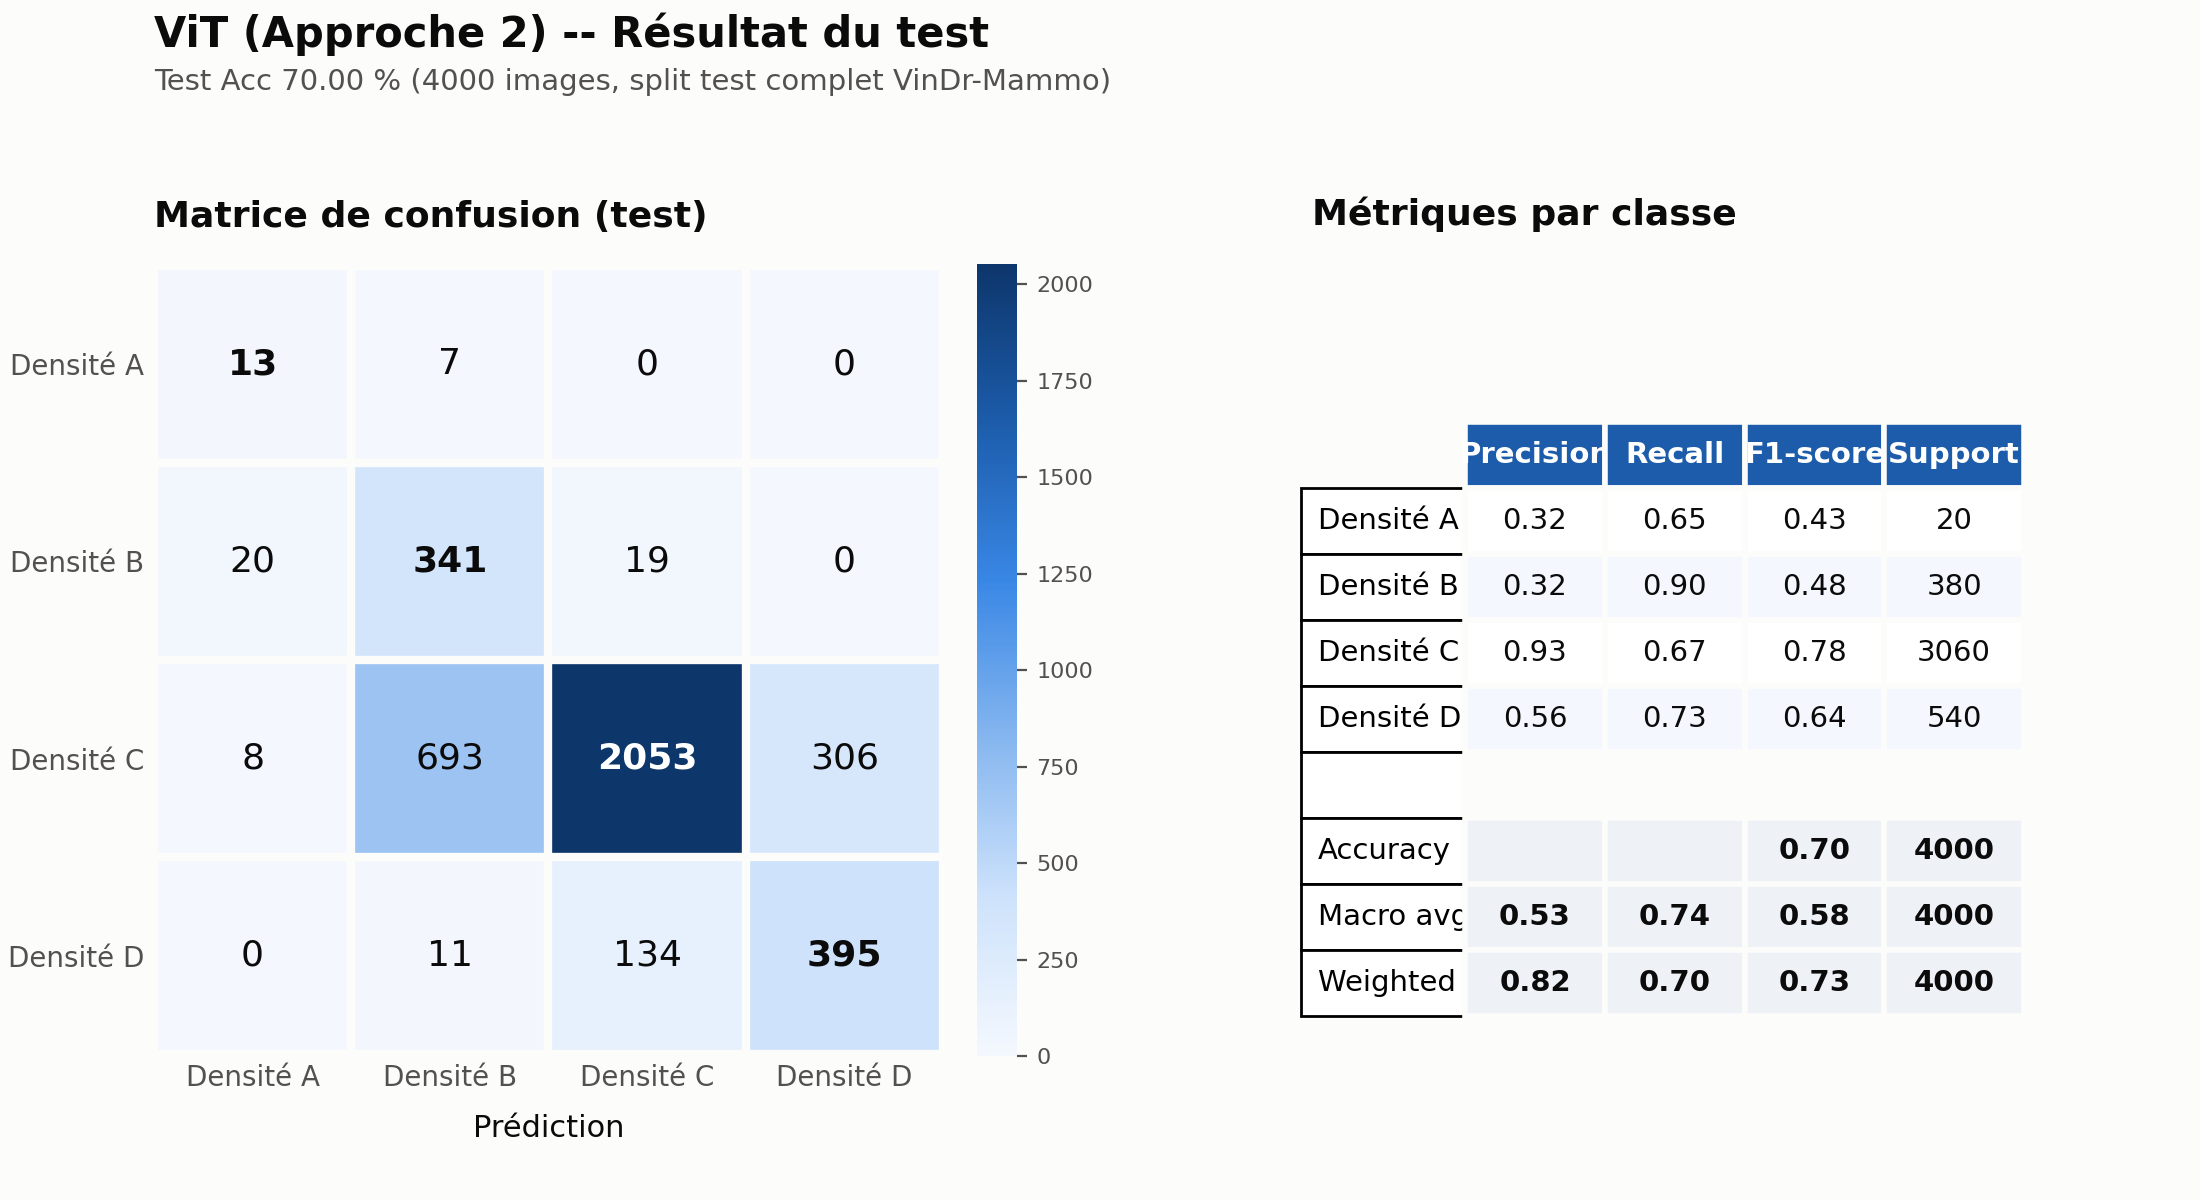
\includegraphics[width=0.75\textwidth]{a2_vit_test}
    \end{center}
\end{frame}

\begin{frame}{Approche 2 -- ResNet50 (fine-tuning direct)}
    \textbf{Test Acc 74.00\,\%} (4000 images) -- \textbf{meilleur rappel classe A de tout le mémoire} (0.95, 19/20)
    \begin{center}
        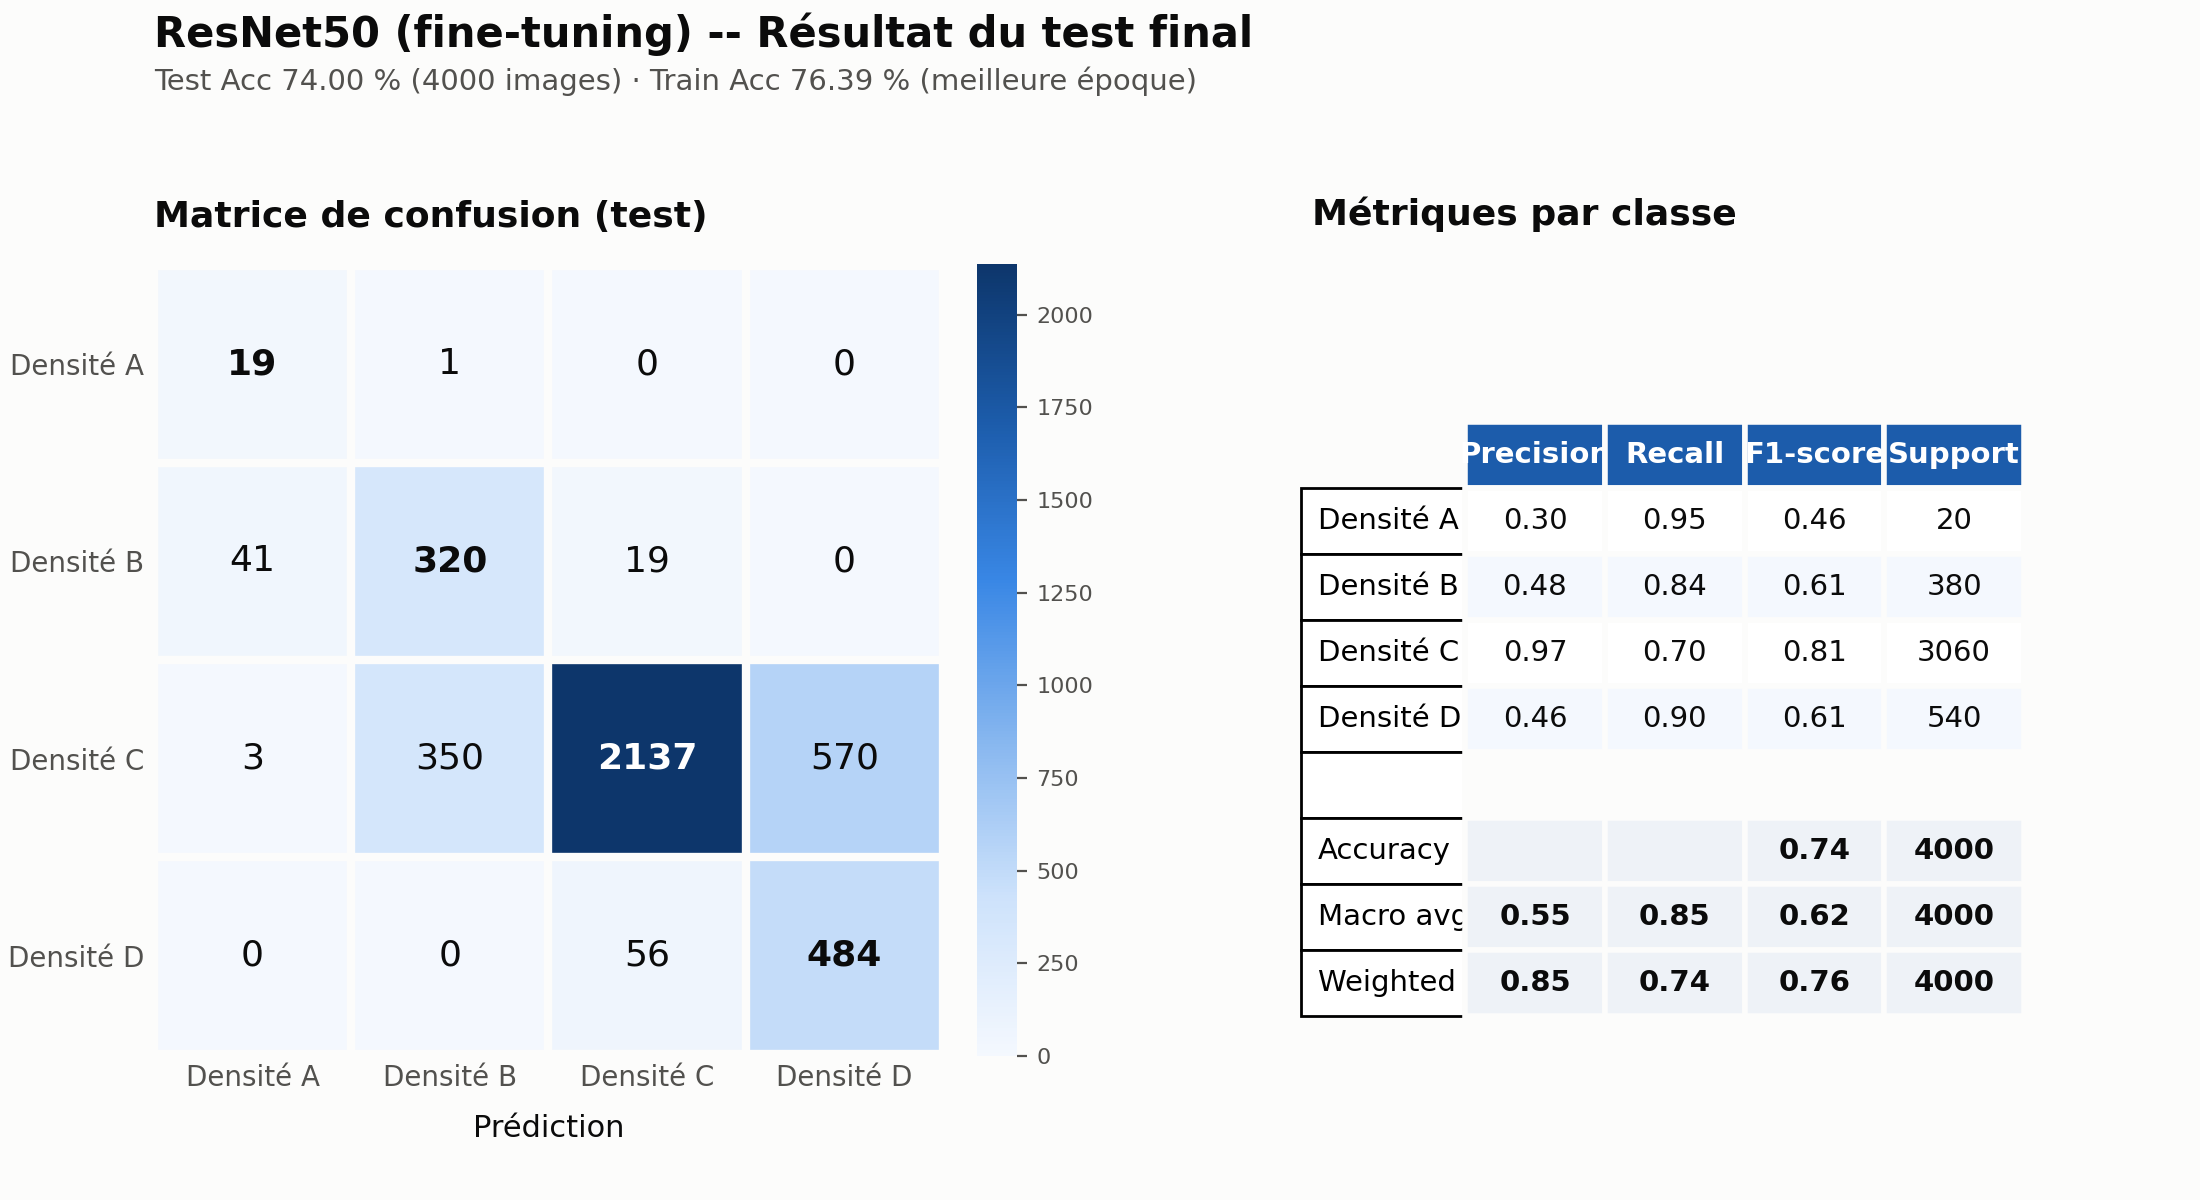
\includegraphics[width=0.75\textwidth]{a2_resnet50_test}
    \end{center}
\end{frame}

% ============================================================================
\section{Approche 3 -- ResNet50 + Histogramme (MLO)}
\begin{frame}{Approche 3 -- ResNet50 + Histogramme (MLO) -- Entraînement}
    Meilleure époque 7/10 -- Val Acc 83.36\,\%
    \begin{center}
        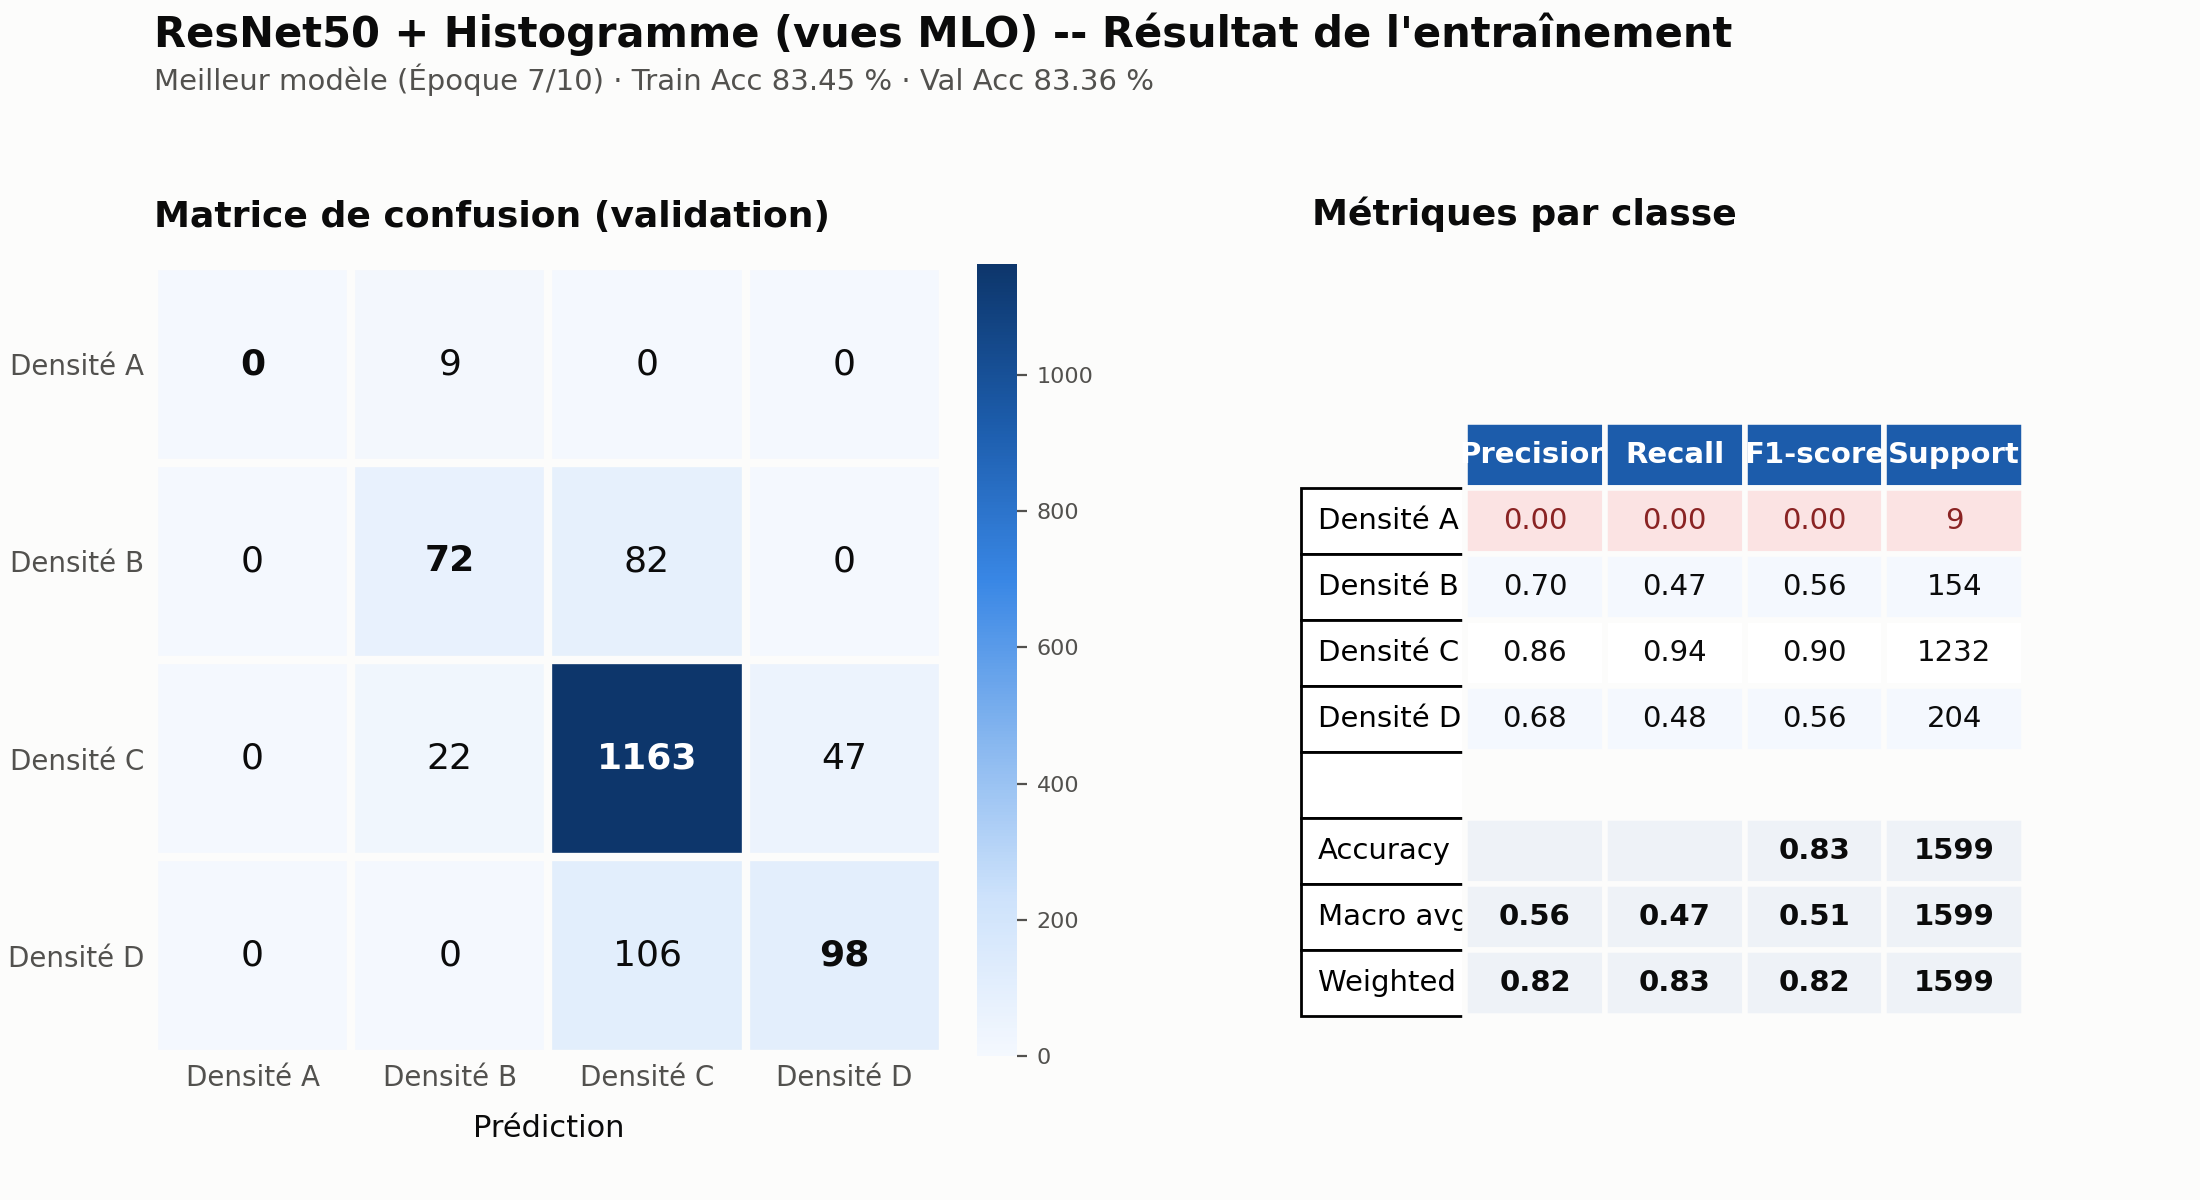
\includegraphics[width=0.7\textwidth]{a3_train}
    \end{center}
\end{frame}

\begin{frame}{Approche 3 -- ResNet50 + Histogramme (MLO) -- Test}
    \textbf{Test Acc 85\,\%} (2000 images MLO) -- \textbf{meilleure accuracy globale du mémoire} -- mais rappel nul sur la classe A
    \begin{center}
        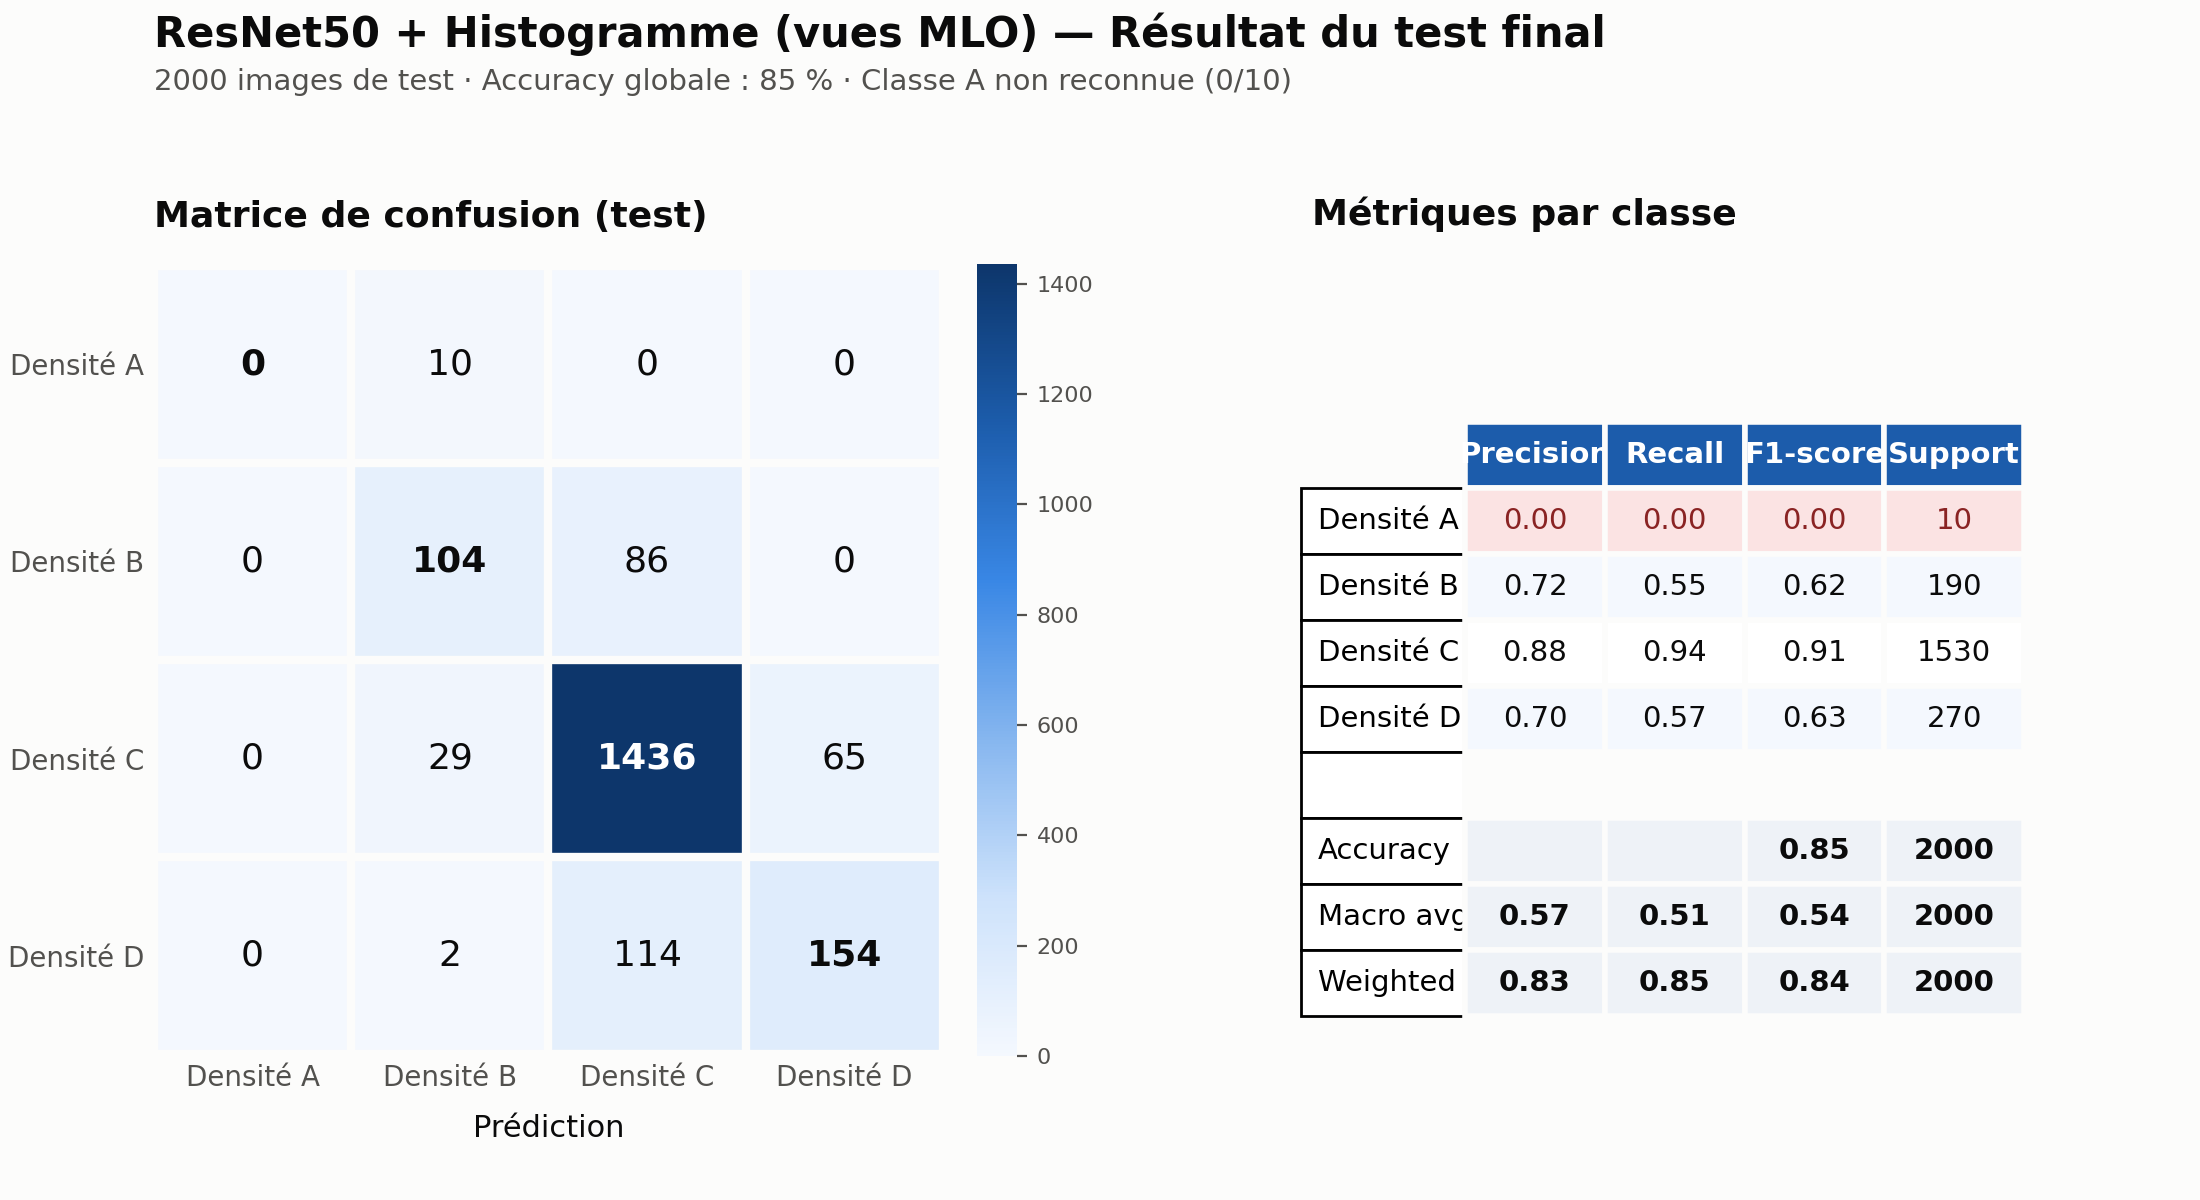
\includegraphics[width=0.7\textwidth]{a3_test}
    \end{center}
\end{frame}

% ============================================================================
\section{Approche 4 -- RexNet150 + Histogramme (CC)}
\begin{frame}{Approche 4 -- RexNet150 + Histogramme (CC) -- Entraînement}
    Meilleure époque 2/5 -- Val Acc 81.56\,\%
    \begin{center}
        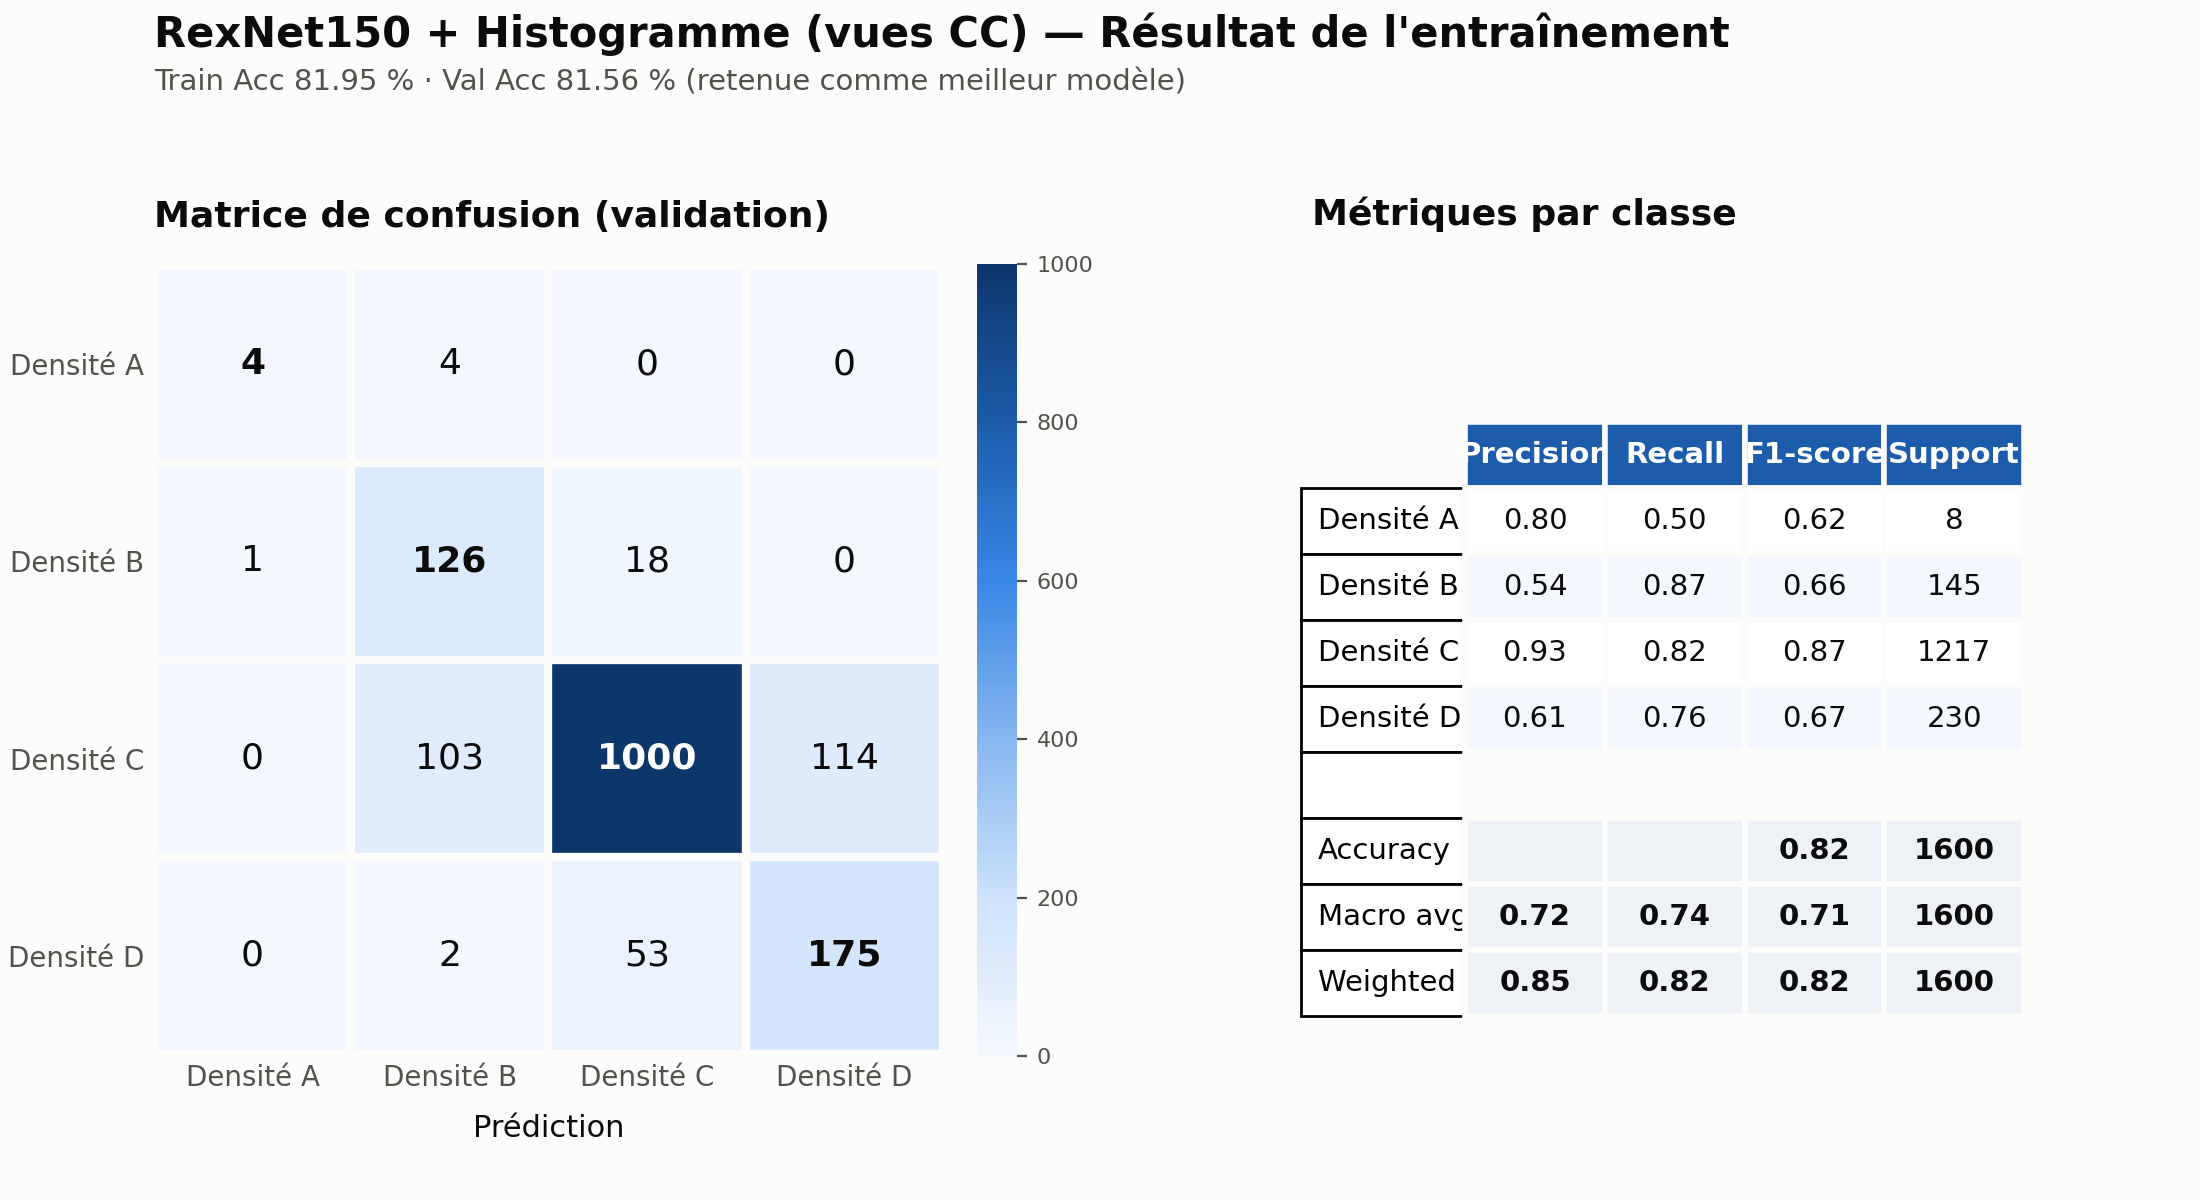
\includegraphics[width=0.7\textwidth]{a4_train}
    \end{center}
\end{frame}

\begin{frame}{Approche 4 -- RexNet150 + Histogramme (CC) -- Test}
    \textbf{Test Acc 80\,\%} (2000 images CC)
    \begin{center}
        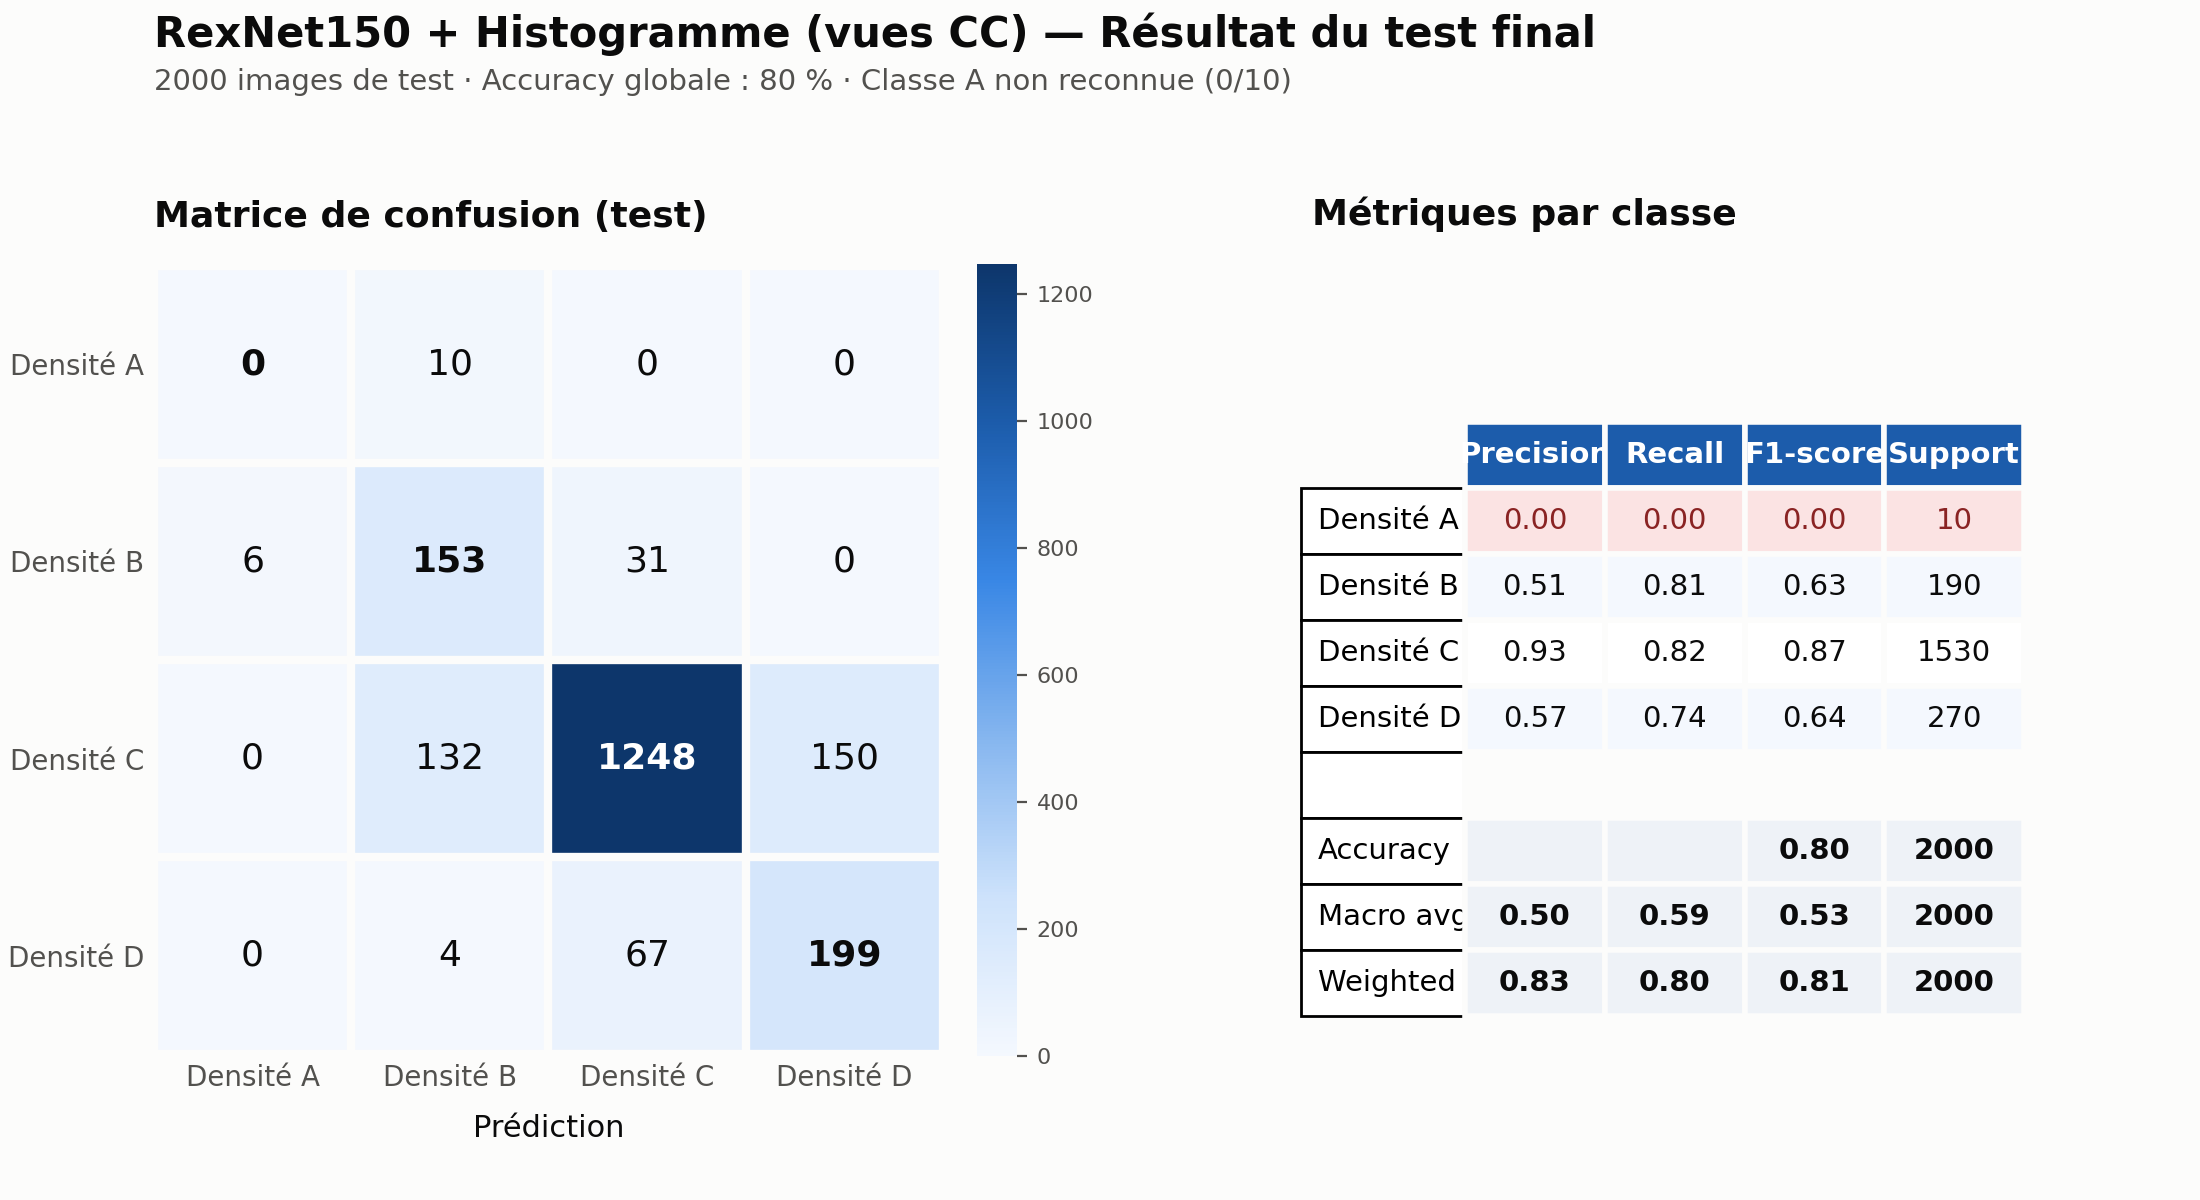
\includegraphics[width=0.7\textwidth]{a4_test}
    \end{center}
\end{frame}

% ============================================================================
\section{Approche 5 -- Branche GLCM}
\begin{frame}{Approche 5 -- Modèle 1 : RexNet150 + GLCM (CC)}
    Val Acc 73.42\,\% -- \textbf{Test Acc 74.85\,\%} (2000 images CC)
    \begin{columns}
        \column{0.5\textwidth}
        \centering \textbf{Entraînement}\\
        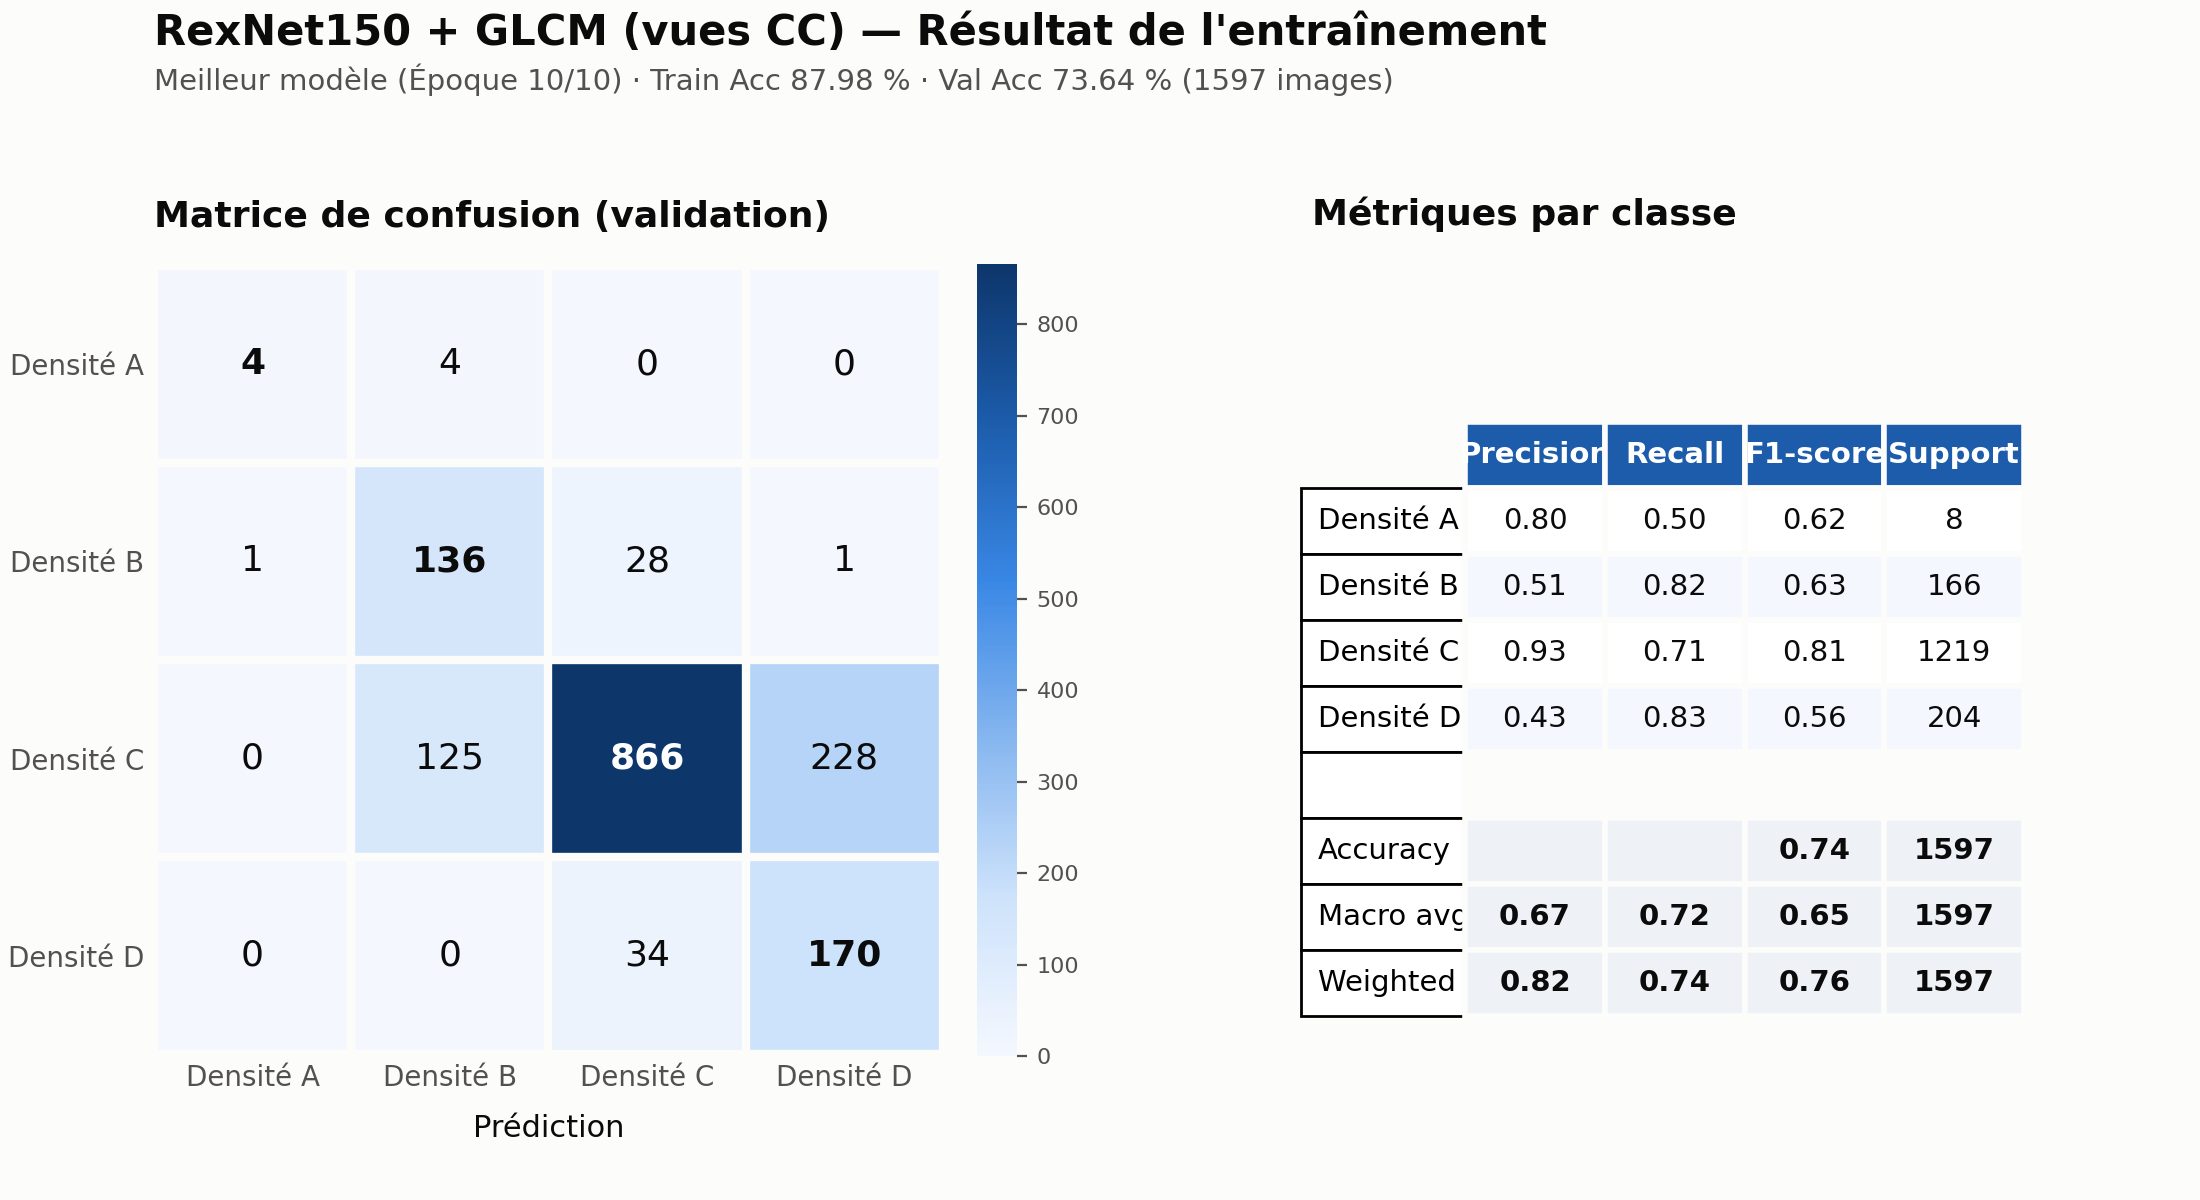
\includegraphics[width=\textwidth]{a5_m1_train}
        \column{0.5\textwidth}
        \centering \textbf{Test}\\
        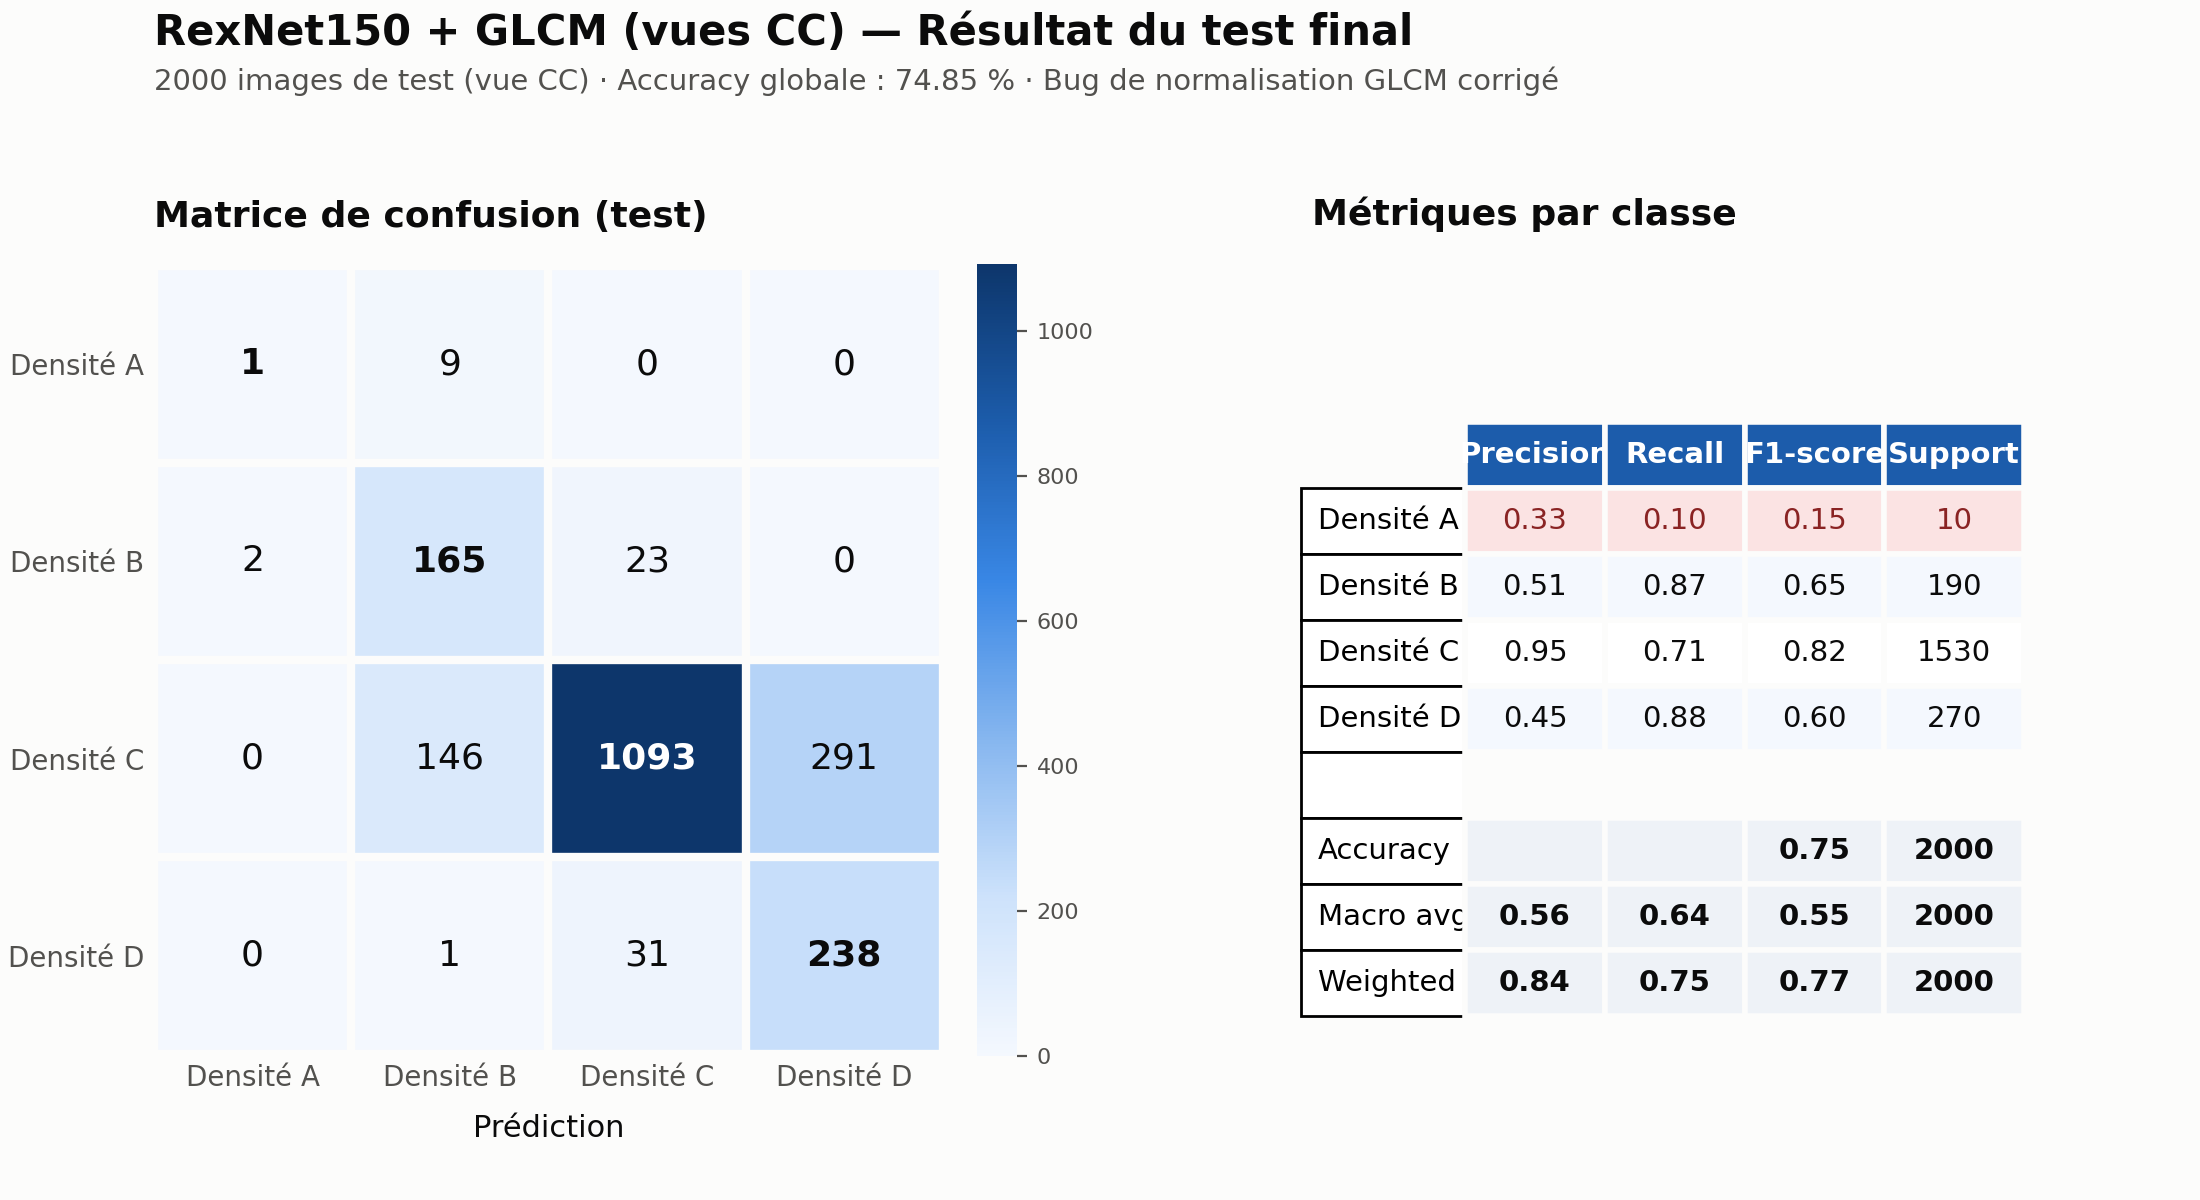
\includegraphics[width=\textwidth]{a5_m1_test}
    \end{columns}
\end{frame}

\begin{frame}{Approche 5 -- Modèle 2 : ResNet50 + GLCM (MLO)}
    Val Acc 72.81\,\% -- \textbf{Test Acc 75.95\,\%} (2000 images MLO)
    \begin{columns}
        \column{0.5\textwidth}
        \centering \textbf{Entraînement}\\
        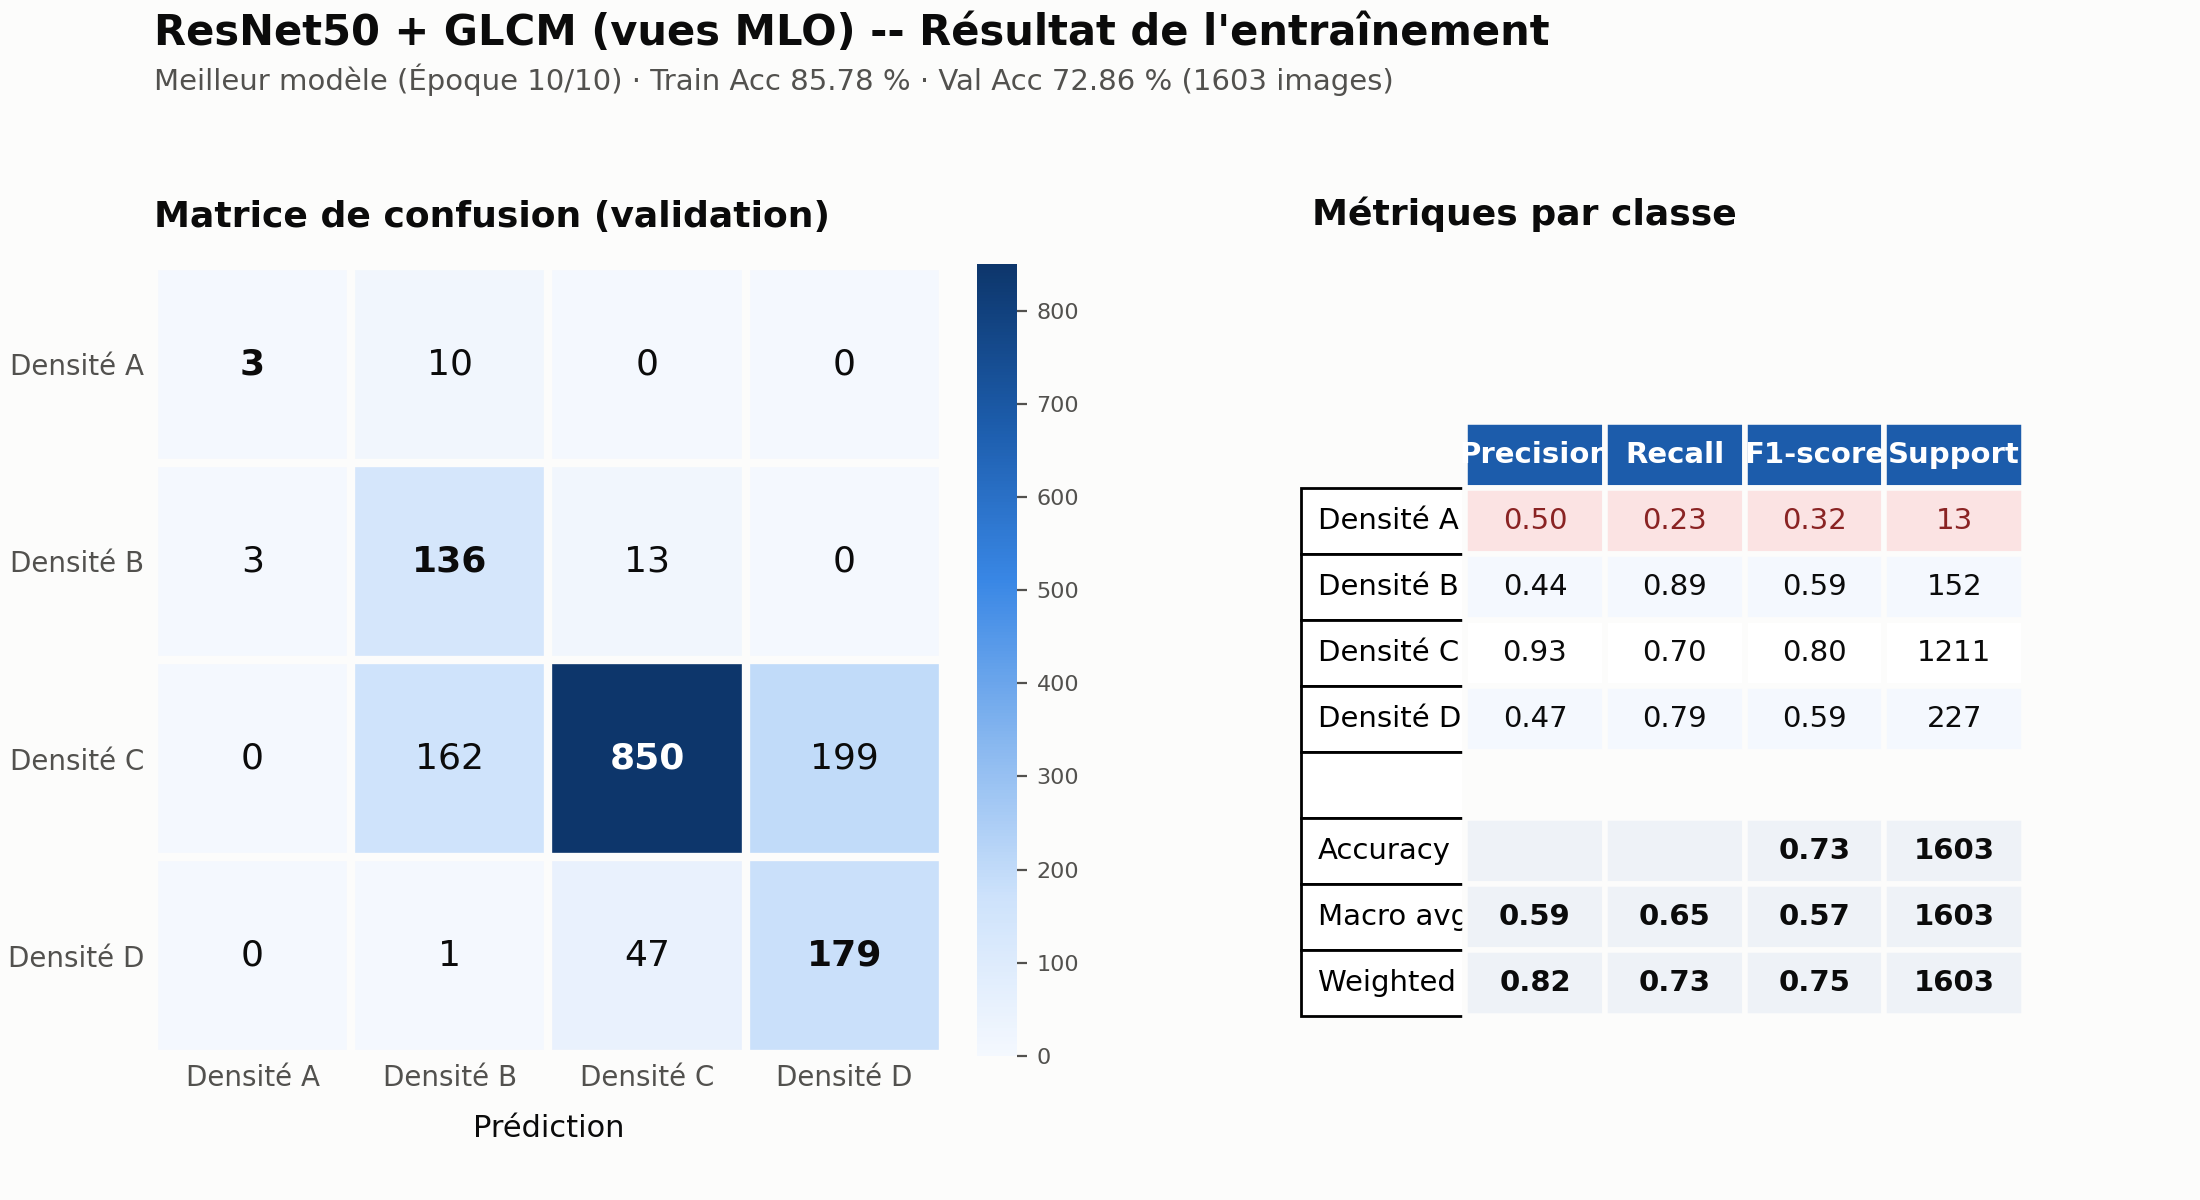
\includegraphics[width=\textwidth]{a5_m2_train}
        \column{0.5\textwidth}
        \centering \textbf{Test}\\
        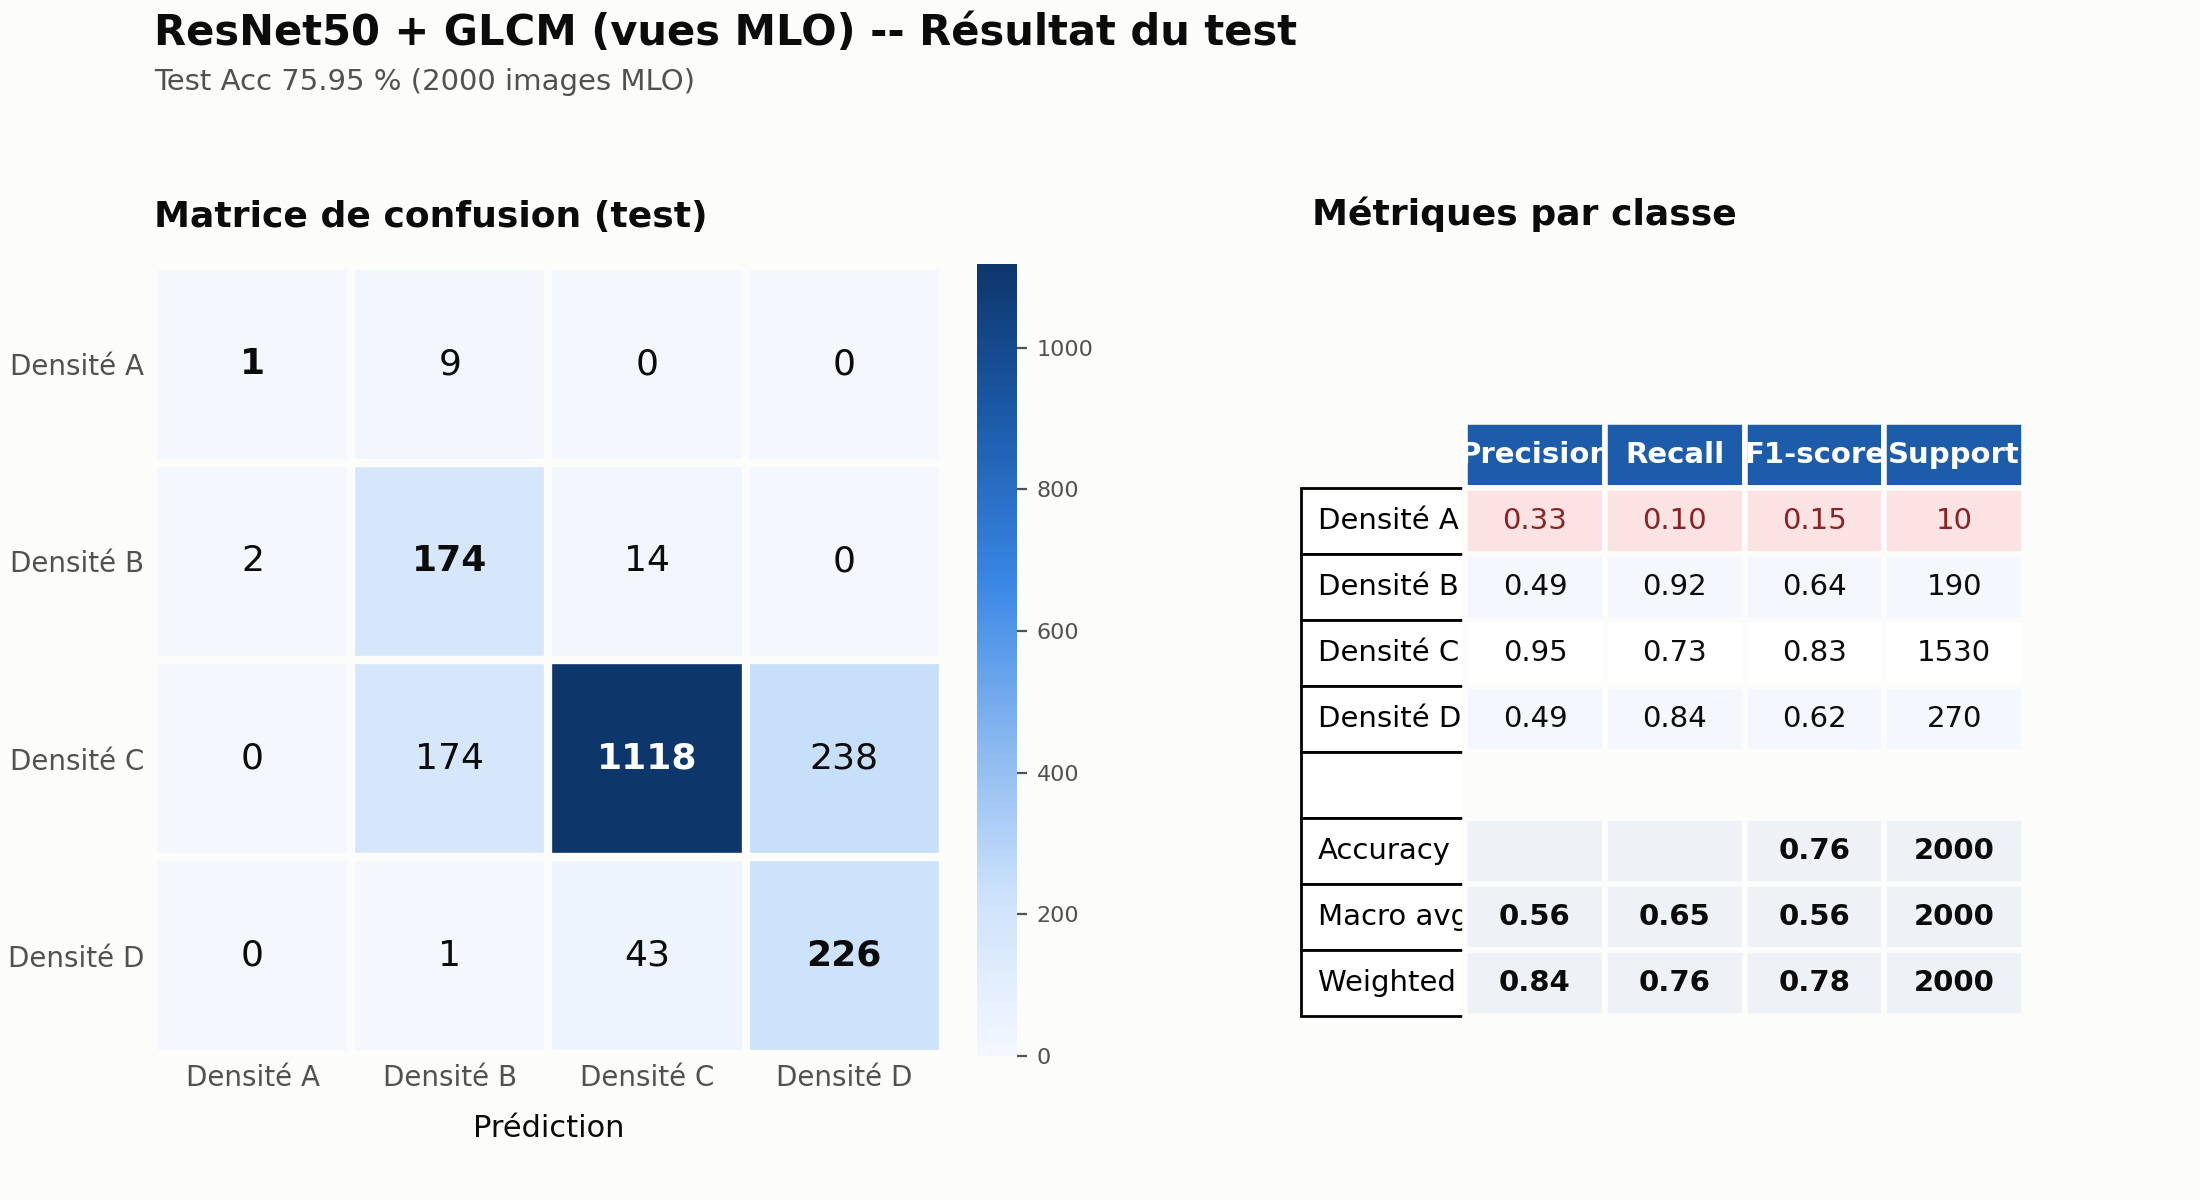
\includegraphics[width=\textwidth]{a5_m2_test}
    \end{columns}
\end{frame}

\begin{frame}{Approche 5 -- Modèle 3 : résultat retiré}
    \begin{alertblock}{Résultat invalidé}
        Le run initial (Train 84.98\,\%, Val 86.68\,\%, Test 84\,\%) chargeait ses
        données depuis un répertoire personnel d'un autre compte du cluster --
        ce n'était pas une réplication indépendante. Résultat retiré du
        mémoire, code corrigé. Faute de temps, pas de réentraînement --
        le principe \og{}Histogramme\fg{} reste couvert par les Approches 3 et 4.
    \end{alertblock}
\end{frame}

% ============================================================================
\section{Approche 6 -- Architecture à double branche}
\begin{frame}{Approche 6 -- Architecture originale (RexNet150/CC + ResNet50/MLO)}
    Val Acc 85.80\,\% (Époque 2/10) -- \textbf{Test Acc 83.00\,\%} (2000 paires)
    \begin{columns}
        \column{0.5\textwidth}
        \centering \textbf{Entraînement}\\
        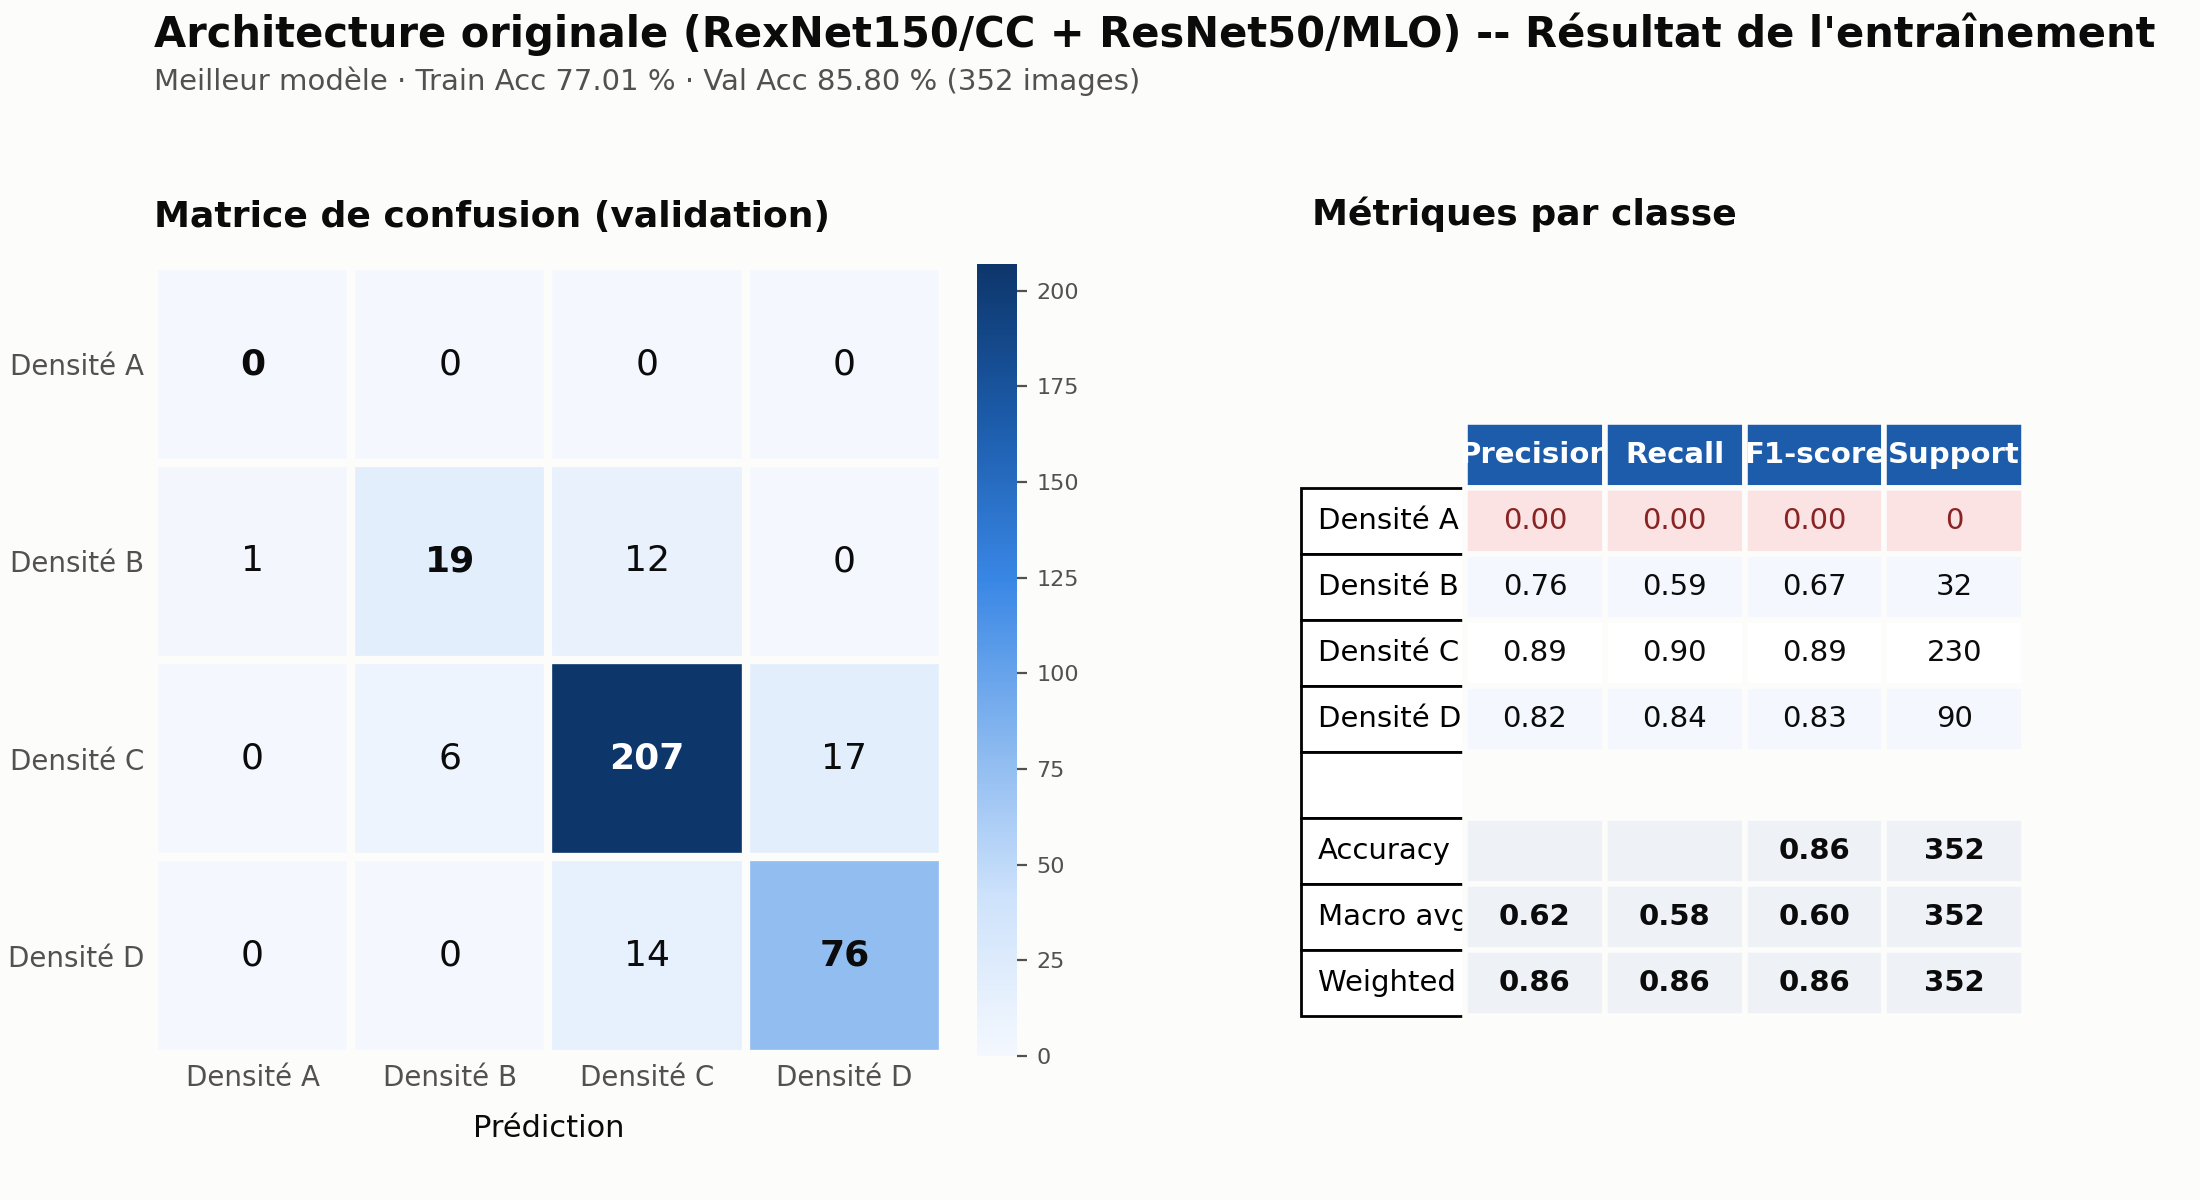
\includegraphics[width=\textwidth]{a6_archi_train}
        \column{0.5\textwidth}
        \centering \textbf{Test}\\
        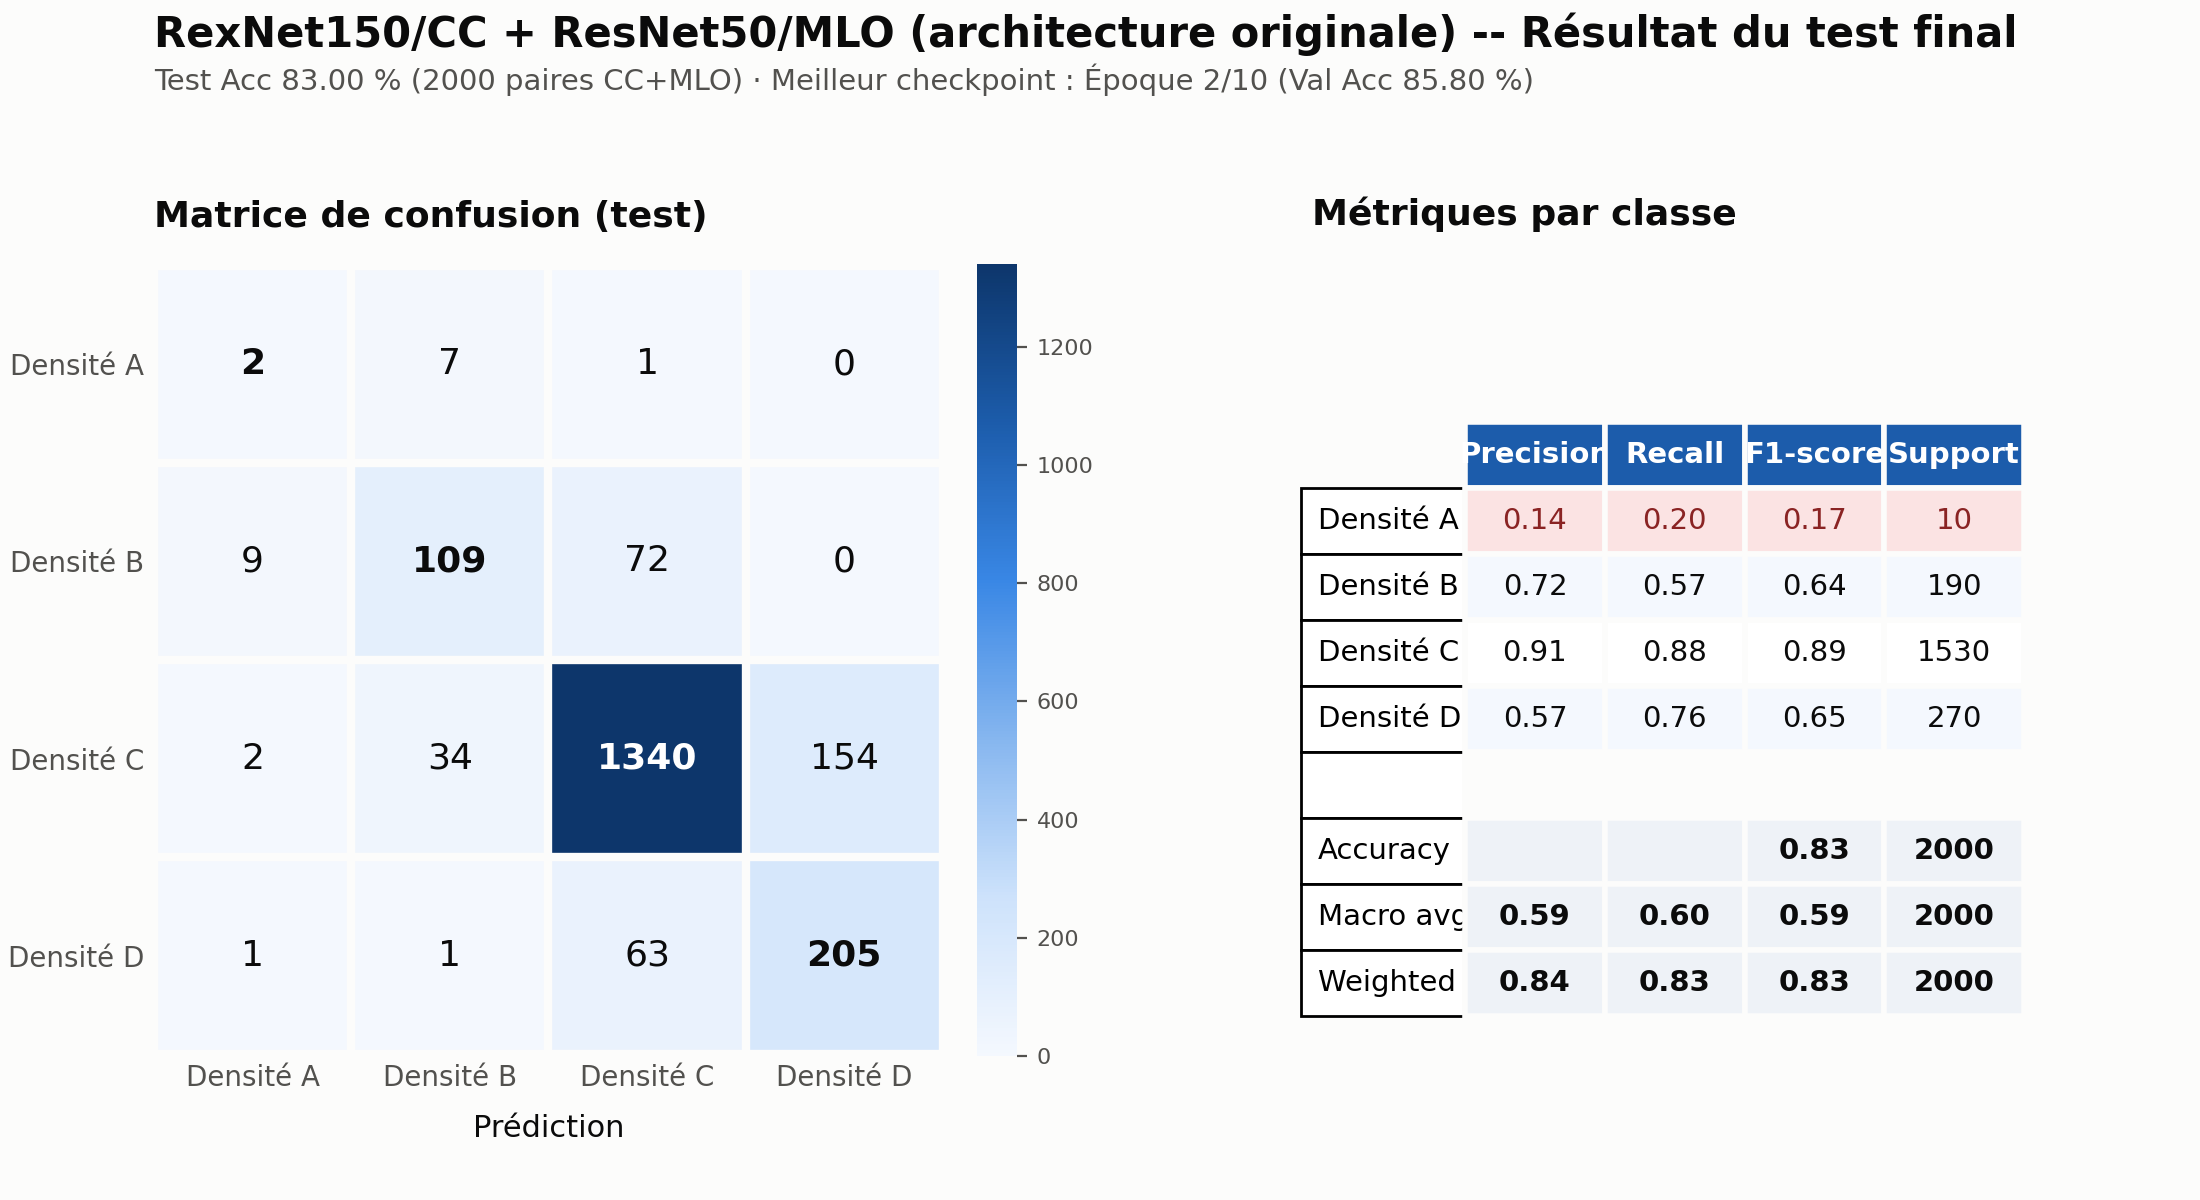
\includegraphics[width=\textwidth]{a6_archi_test}
    \end{columns}
\end{frame}

\begin{frame}{Approche 6 -- Variante siamoise (EfficientNet-B0, poids partagés)}
    Val Acc 84.38\,\% (Époque 4/10) -- \textbf{Test Acc 85.00\,\%} -- meilleur résultat des 4 variantes
    \begin{columns}
        \column{0.5\textwidth}
        \centering \textbf{Entraînement}\\
        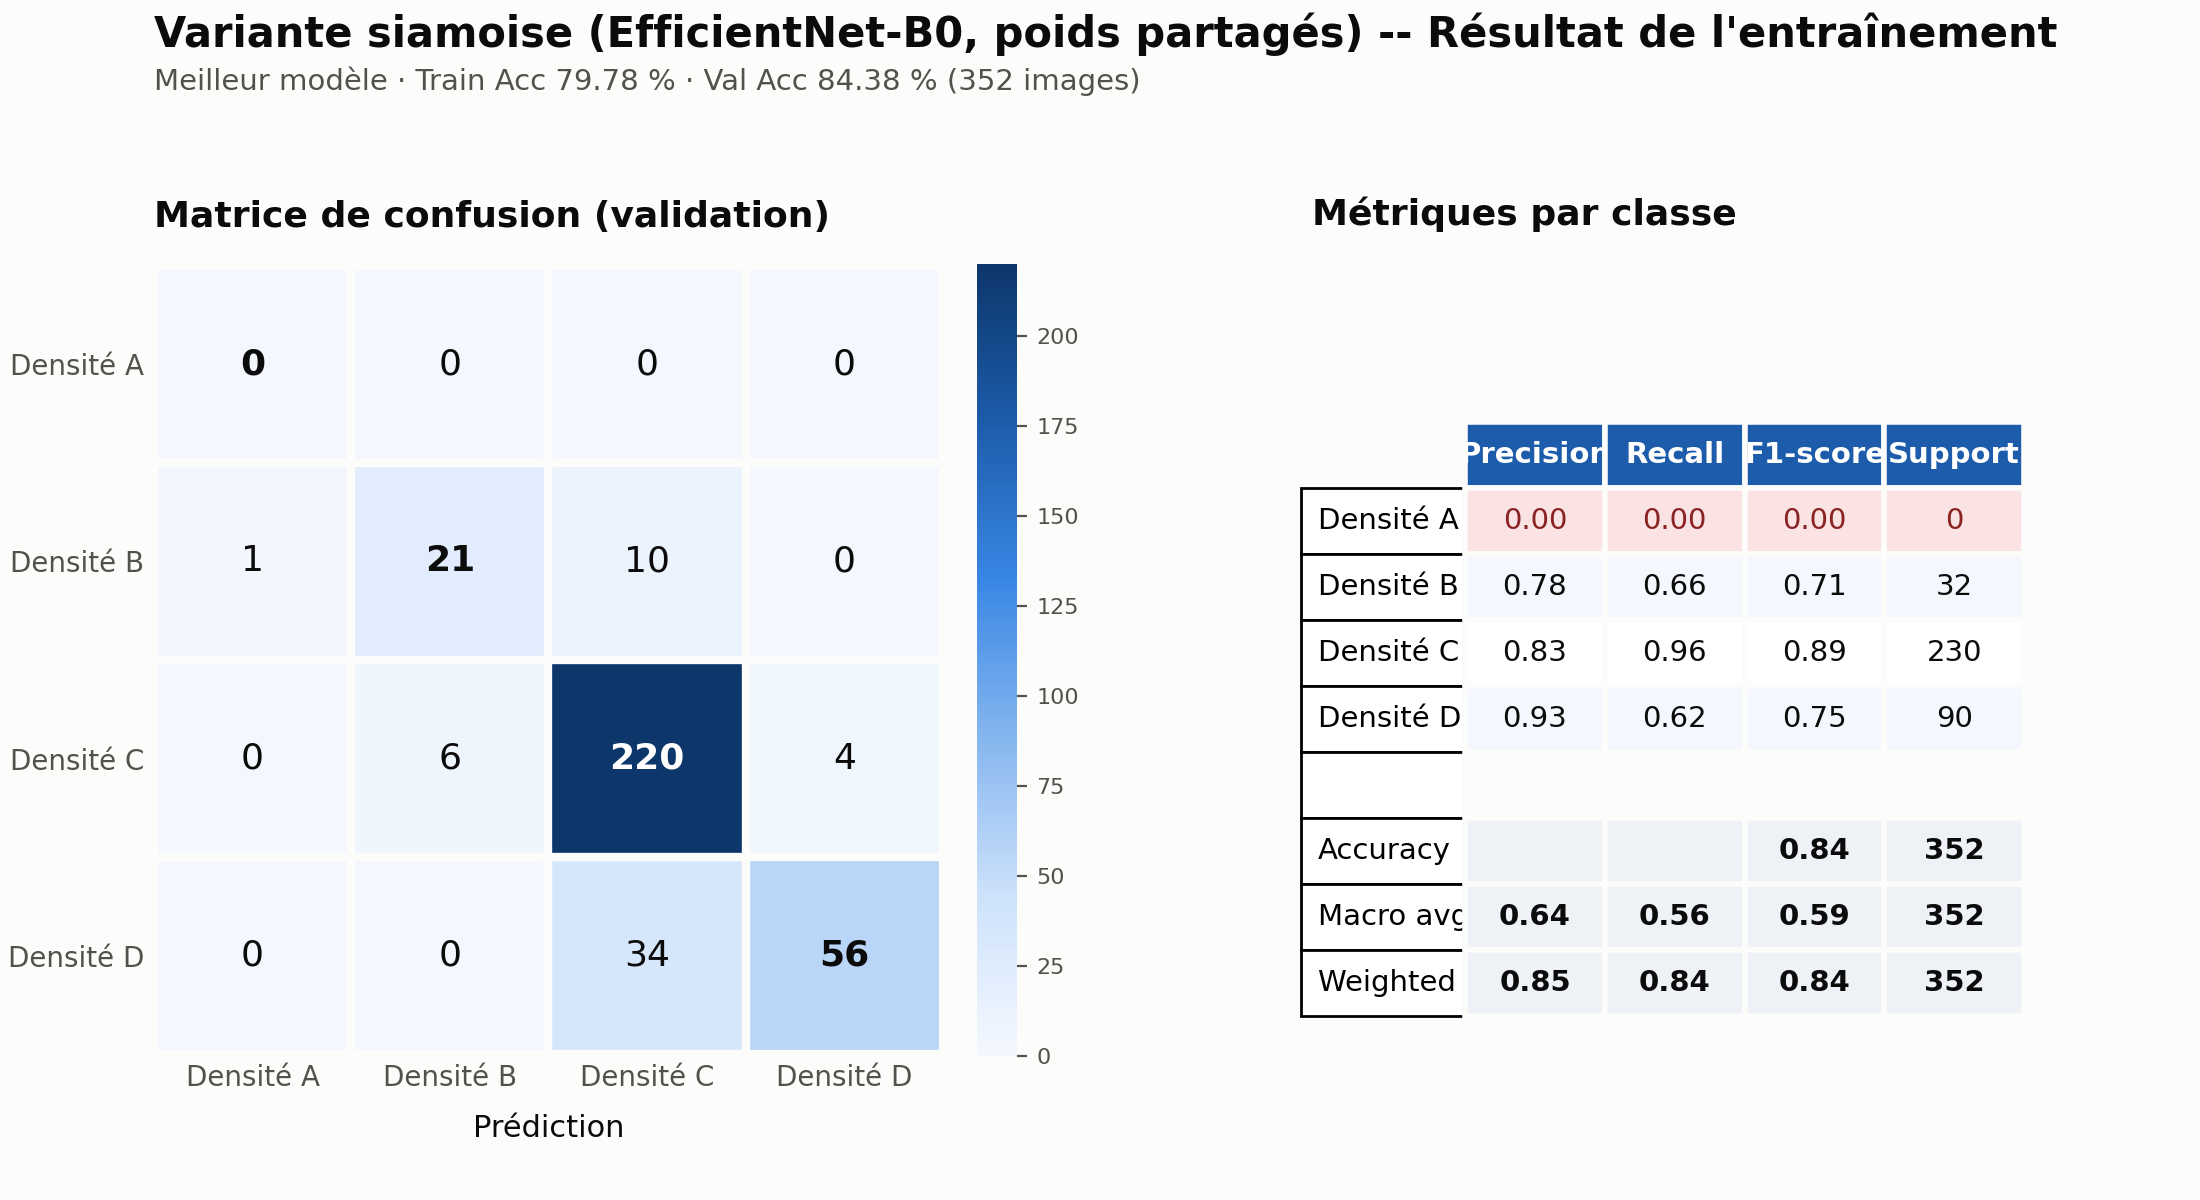
\includegraphics[width=\textwidth]{a6_siam_train}
        \column{0.5\textwidth}
        \centering \textbf{Test}\\
        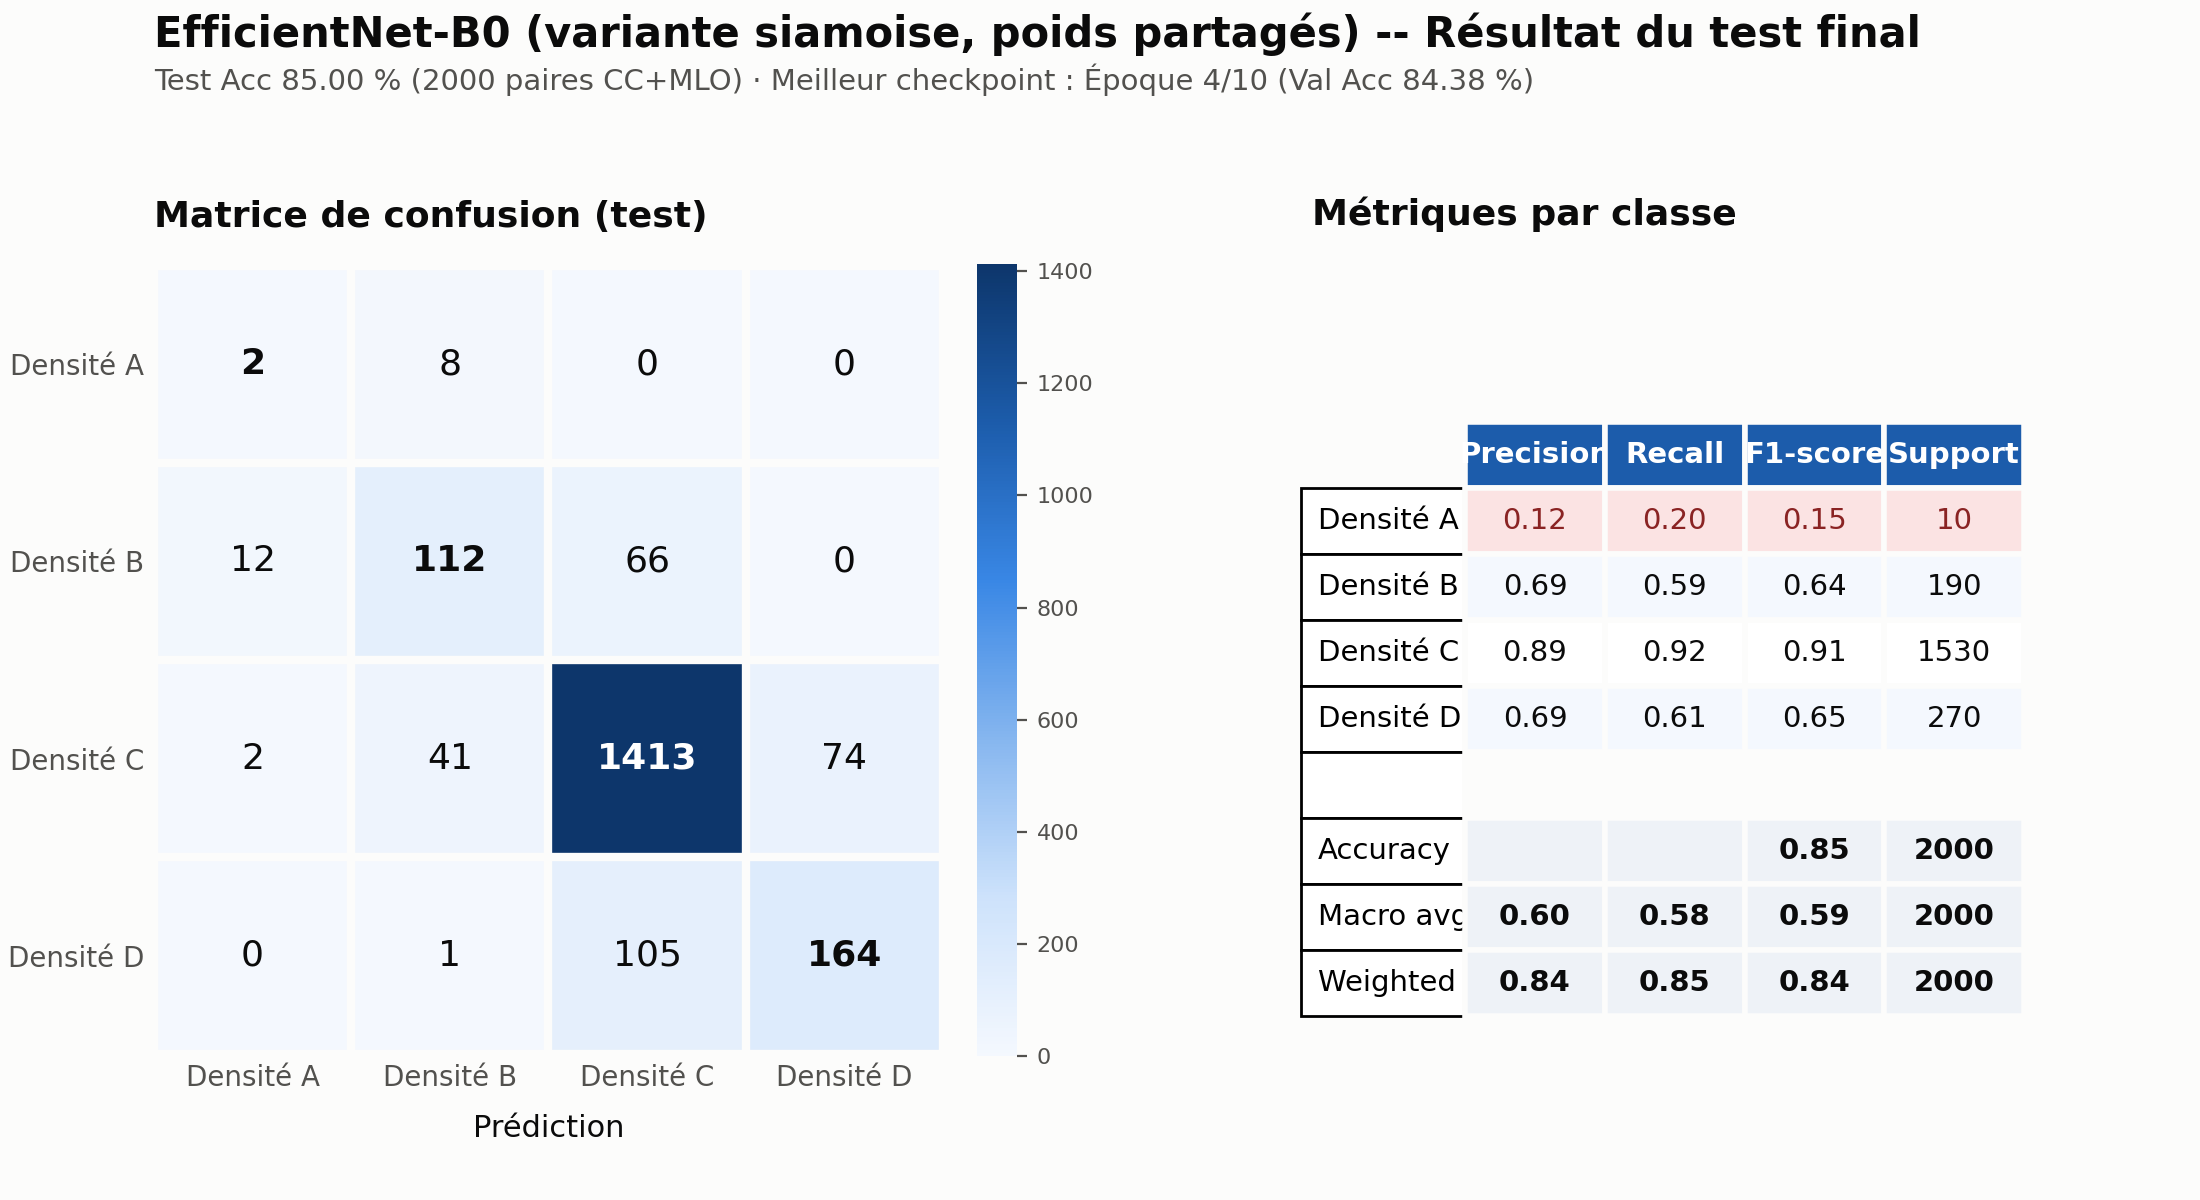
\includegraphics[width=\textwidth]{a6_siam_test}
    \end{columns}
\end{frame}

\begin{frame}{Approche 6 -- Fusion même-vue : RexNet150 + ResNet50 (MLO)}
    Val Acc 74.62\,\% -- \textbf{Test Acc 74.85\,\%} (2000 images MLO)
    \begin{columns}
        \column{0.5\textwidth}
        \centering \textbf{Entraînement}\\
        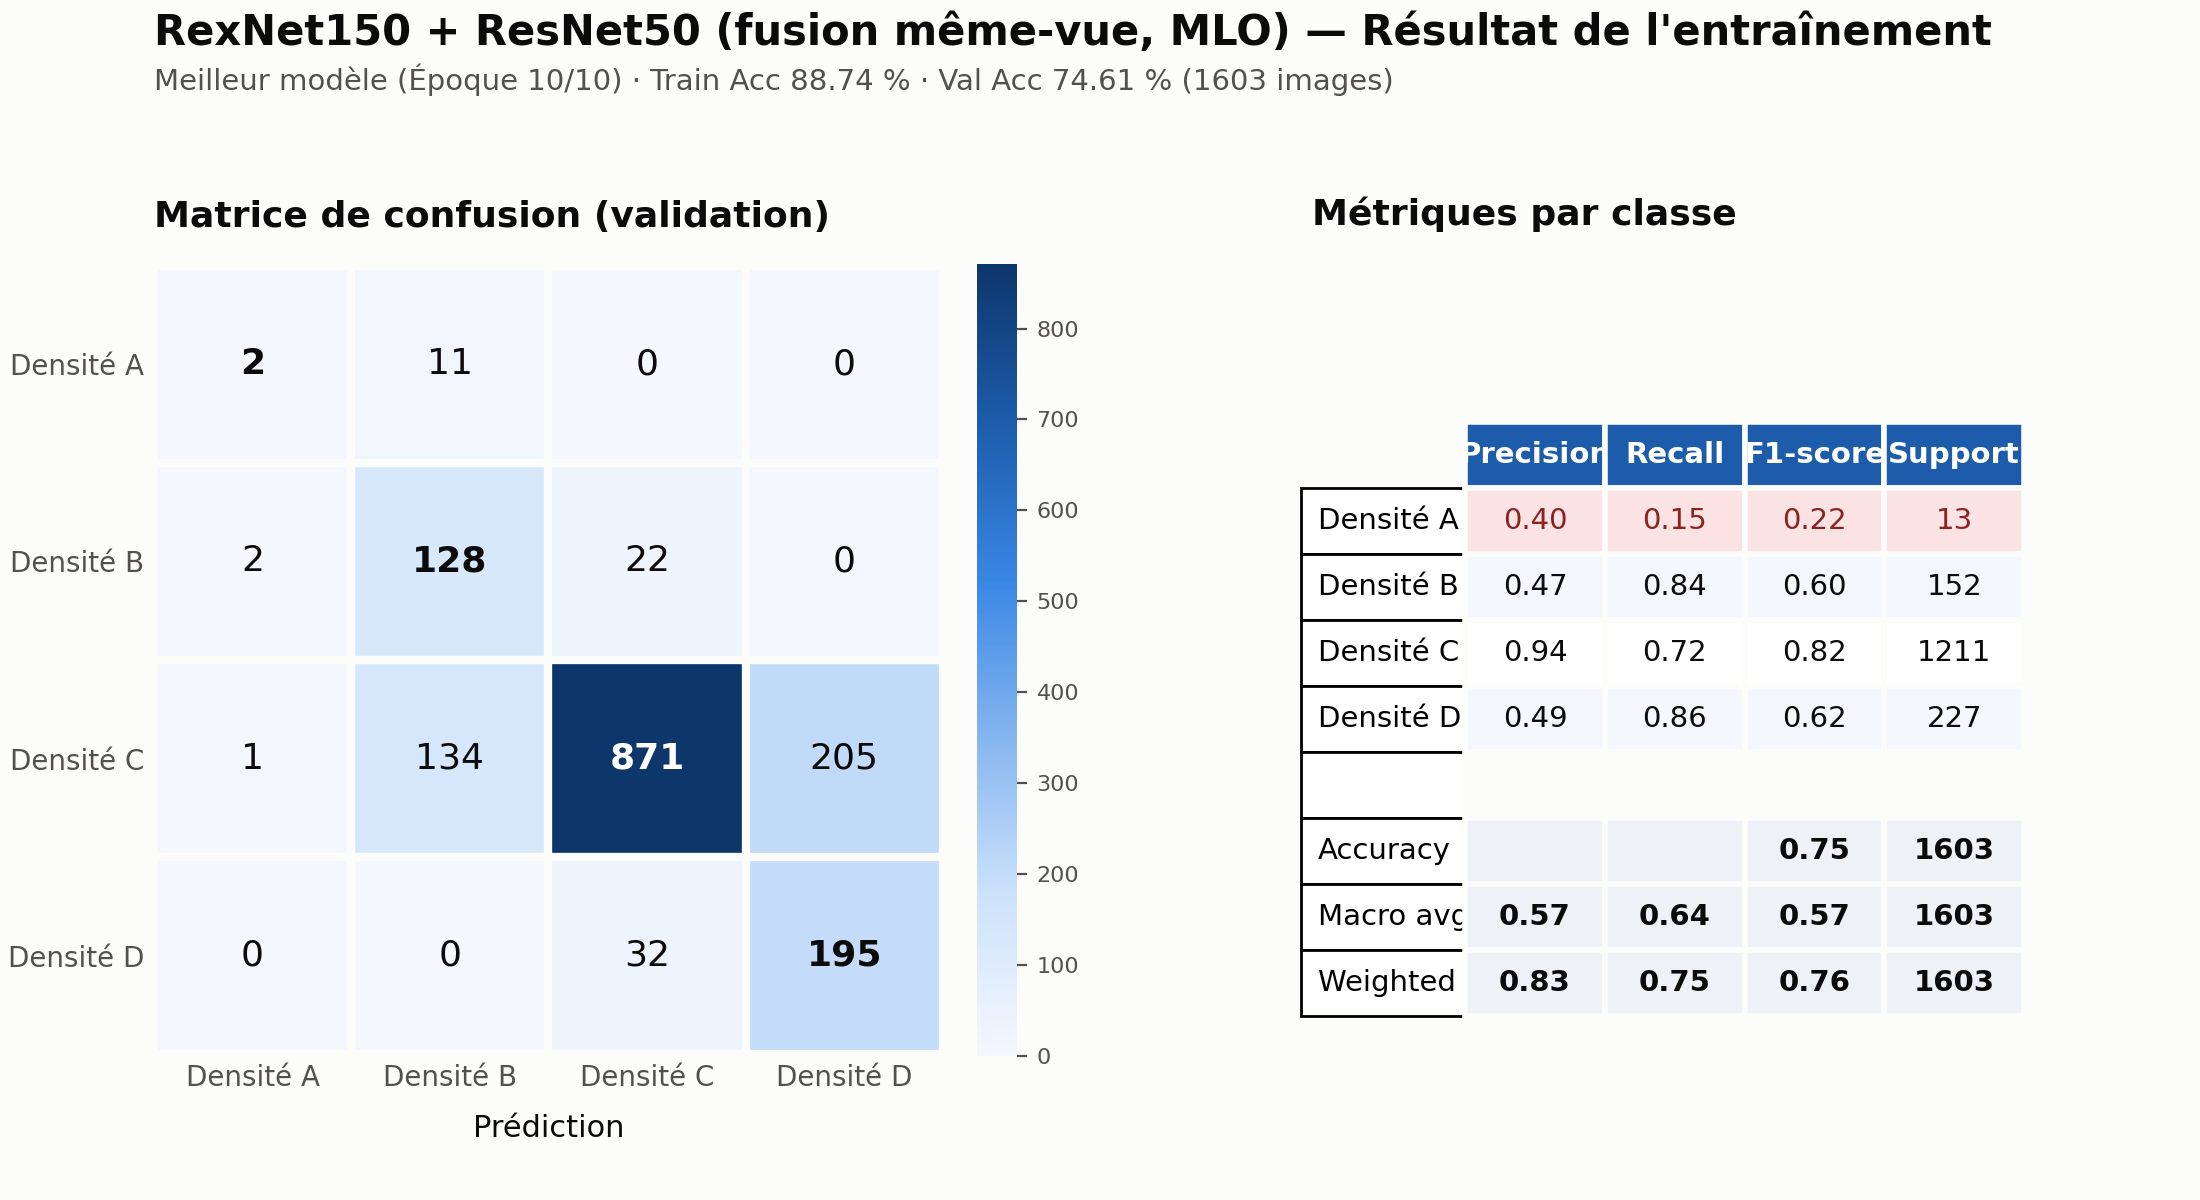
\includegraphics[width=\textwidth]{a6_mlo_train}
        \column{0.5\textwidth}
        \centering \textbf{Test}\\
        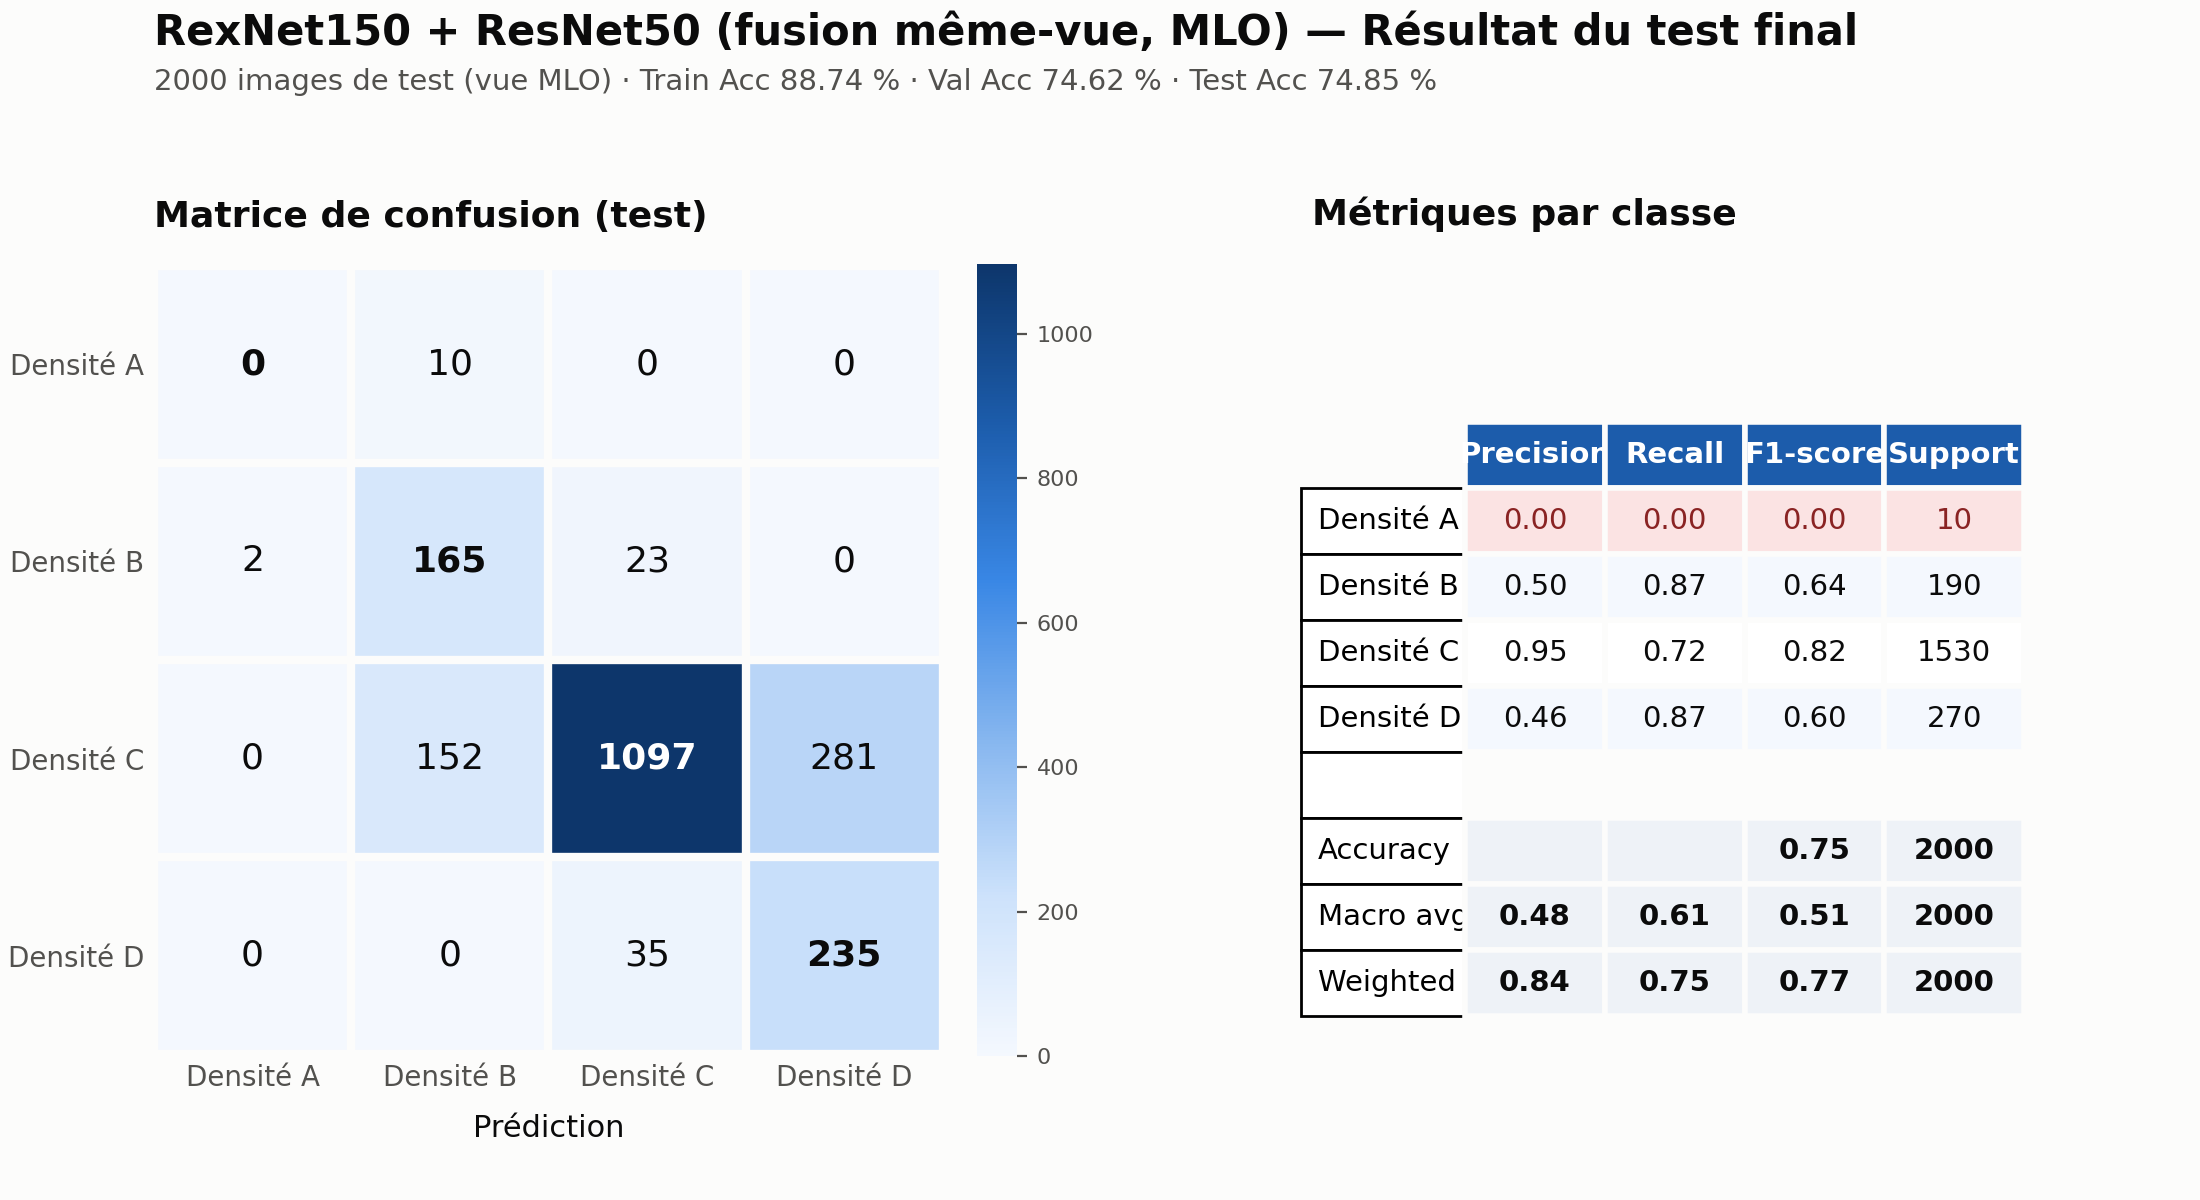
\includegraphics[width=\textwidth]{a6_mlo_test}
    \end{columns}
\end{frame}

\begin{frame}{Approche 6 -- Fusion même-vue : DenseNet121 + ResNet50 (CC)}
    Val Acc 75.69\,\% -- \textbf{Test Acc 76.35\,\%} (2000 images CC)
    \begin{columns}
        \column{0.5\textwidth}
        \centering \textbf{Entraînement}\\
        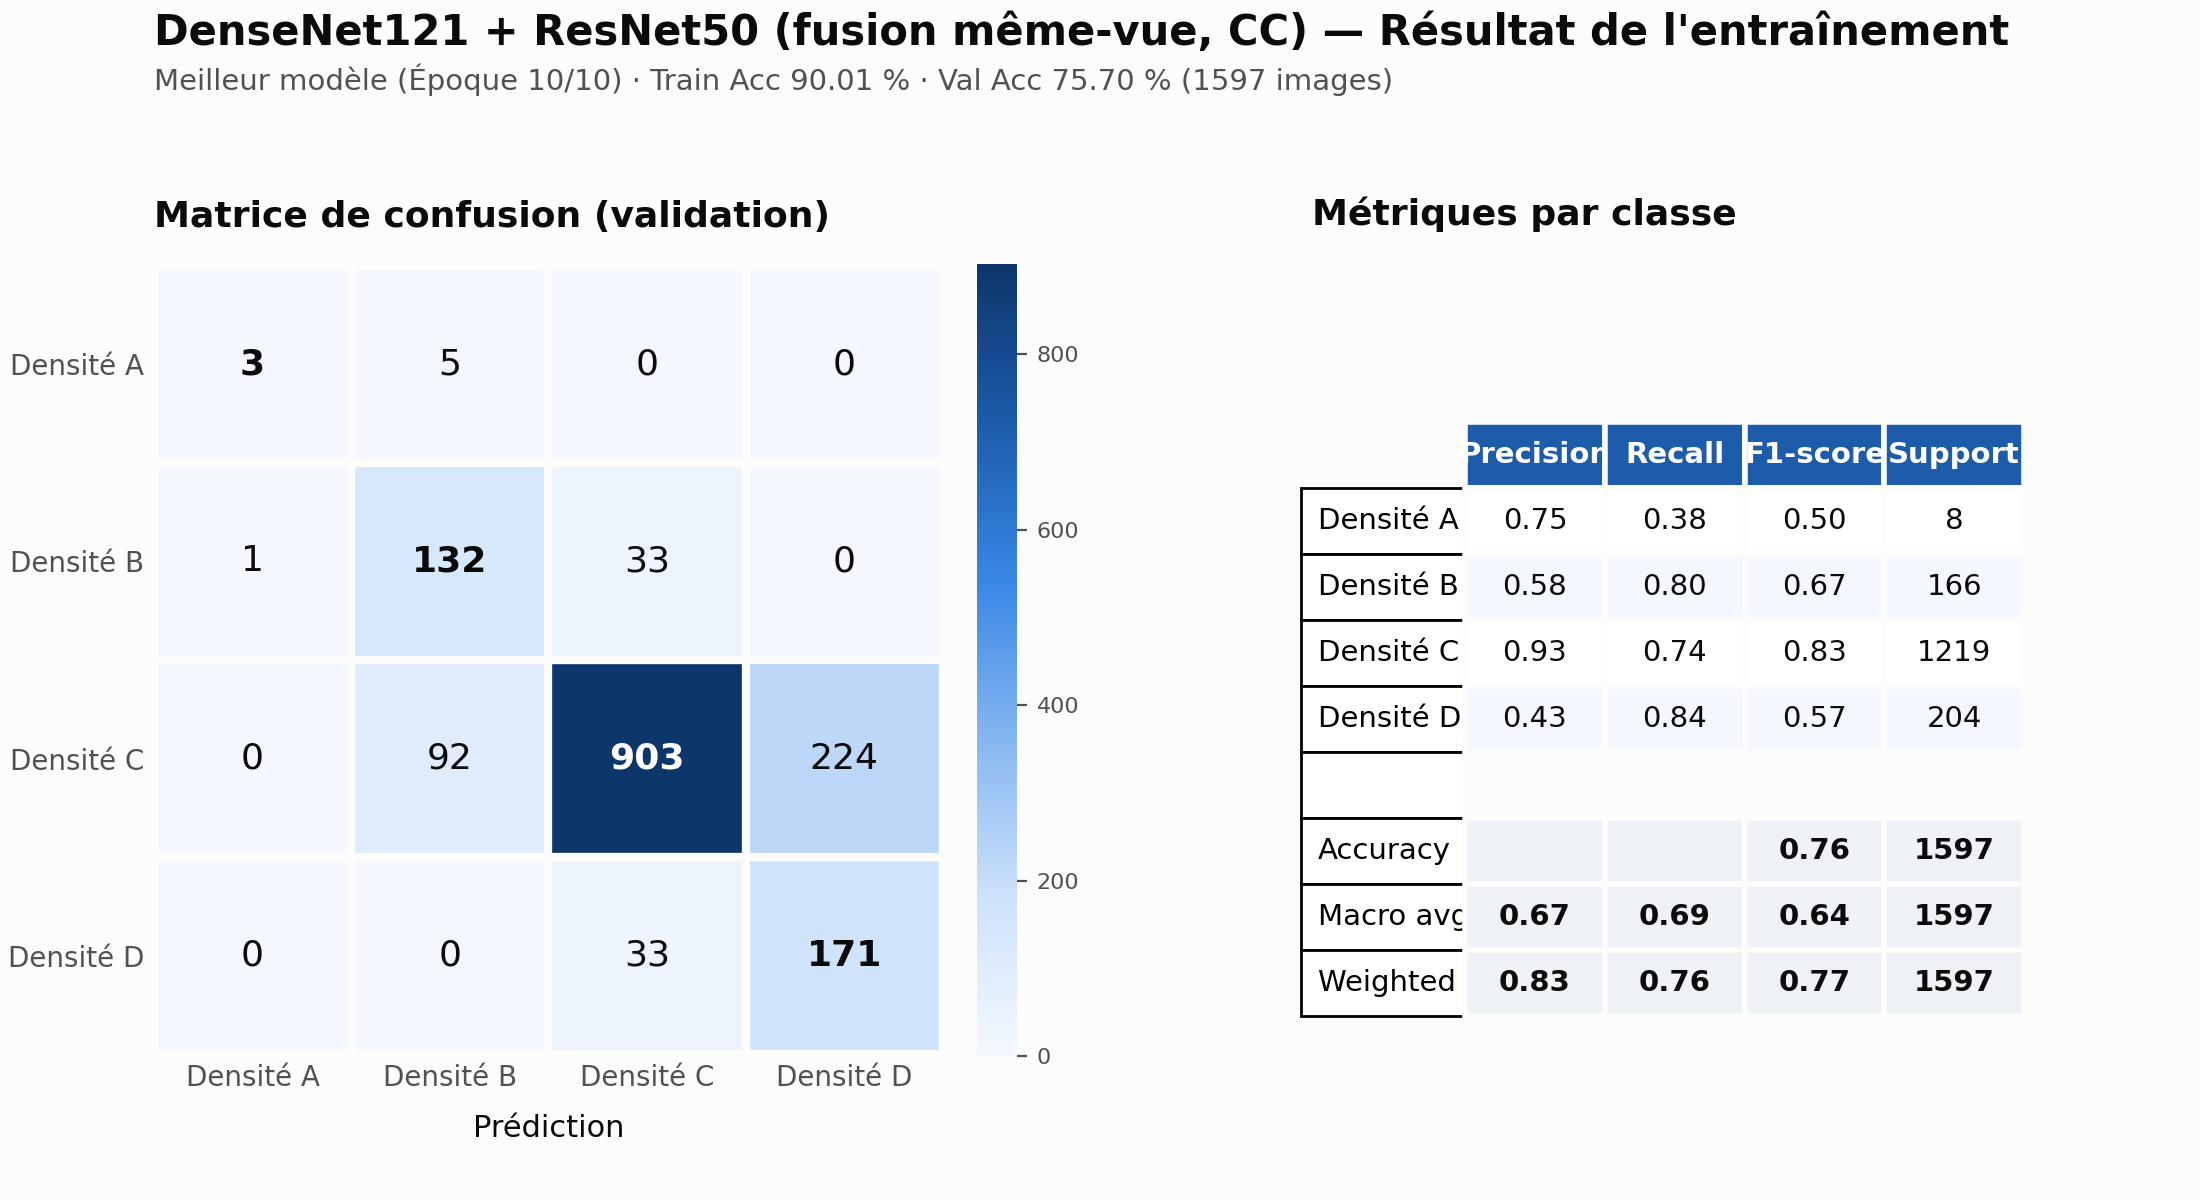
\includegraphics[width=\textwidth]{a6_cc_train}
        \column{0.5\textwidth}
        \centering \textbf{Test}\\
        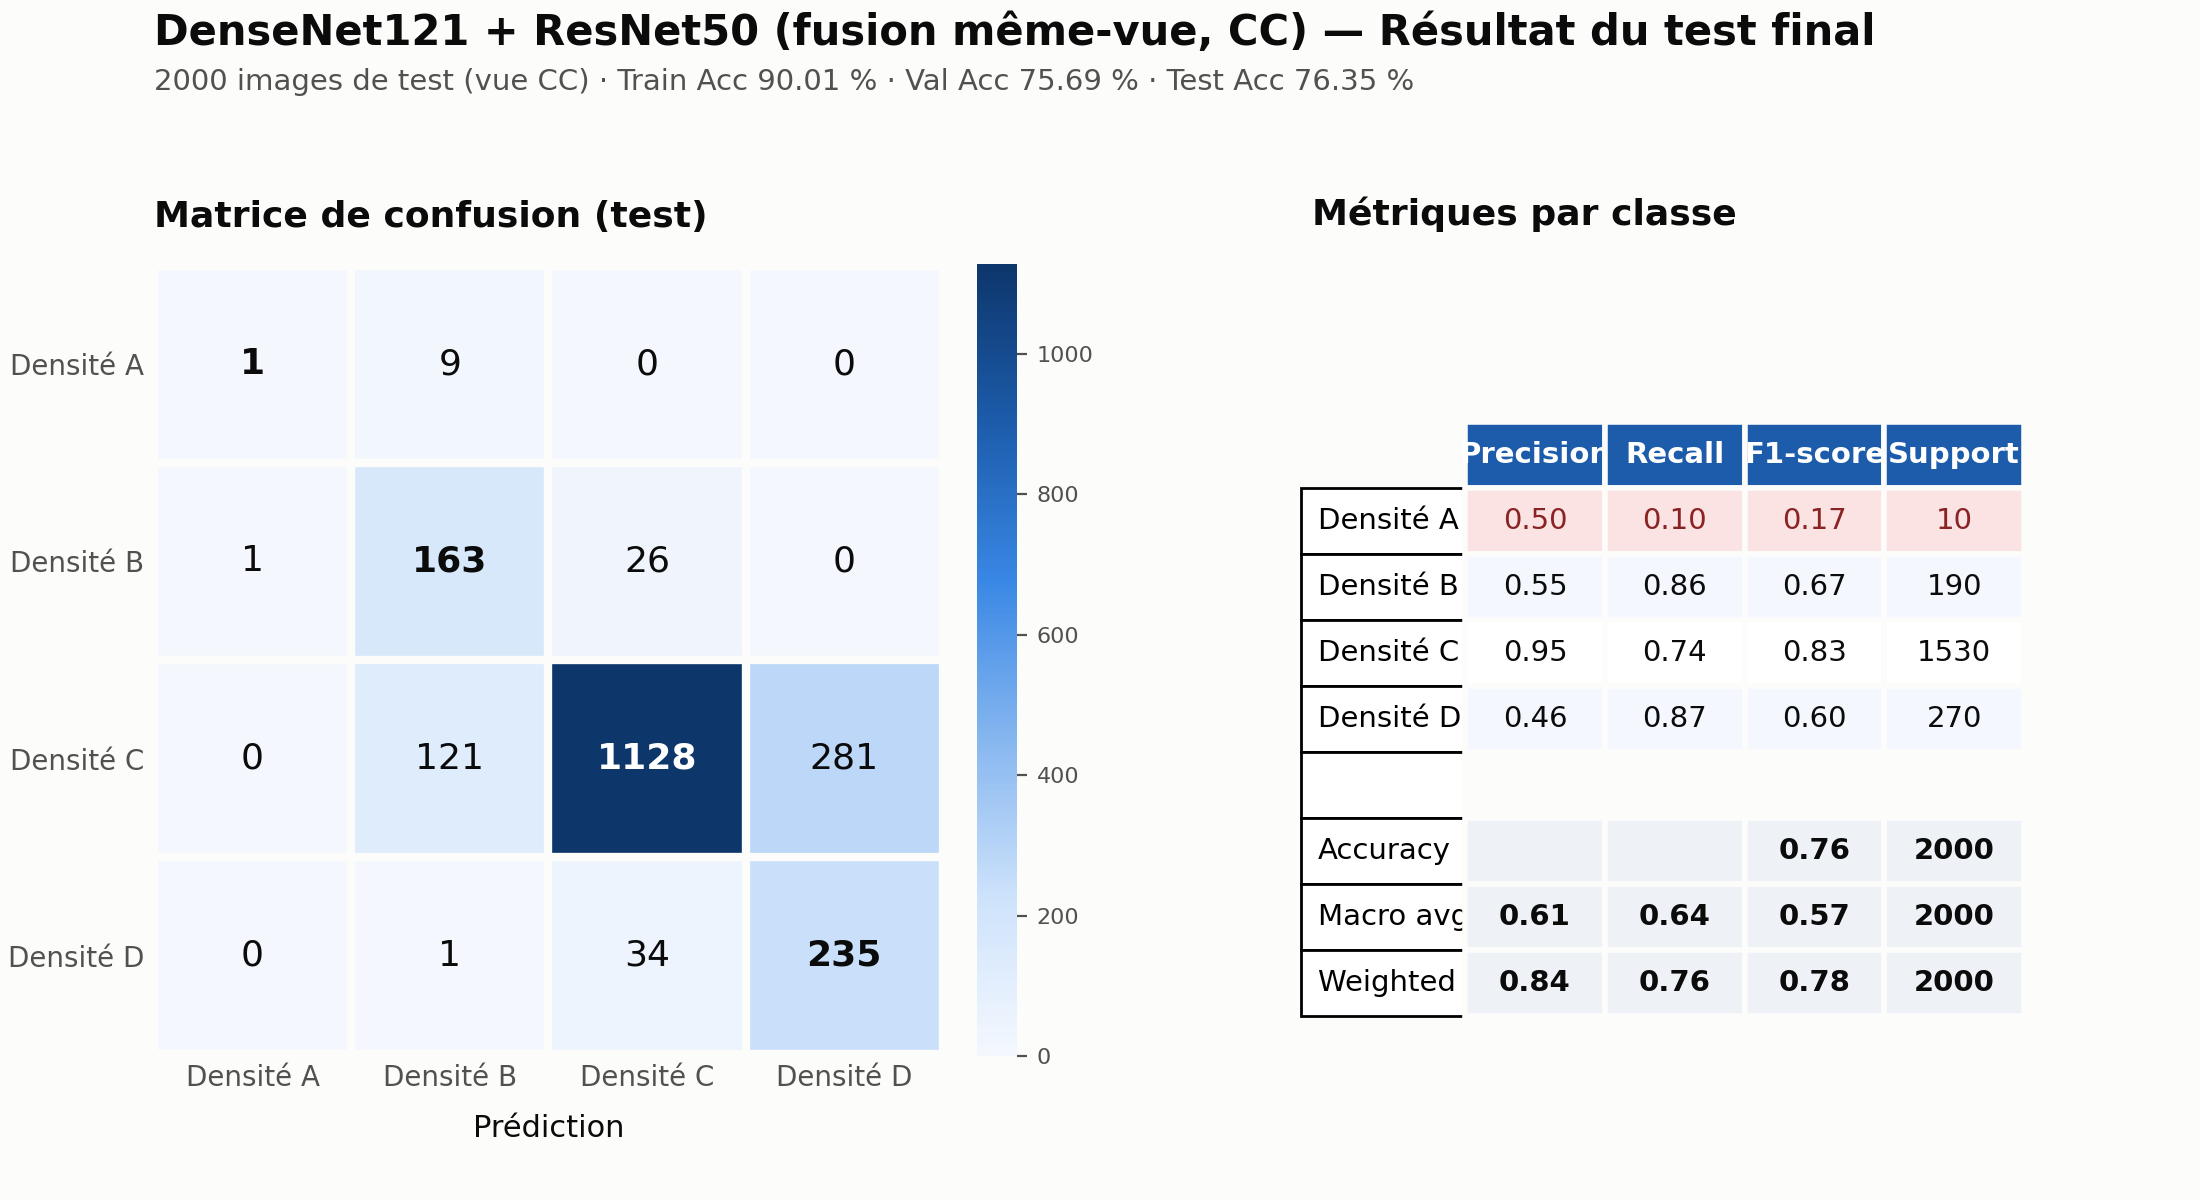
\includegraphics[width=\textwidth]{a6_cc_test}
    \end{columns}
\end{frame}

\begin{frame}{Approche 6 -- Synthèse}
    \begin{table}
    \centering
    \begin{tabular}{lrrr}
        \toprule
        Variante & Train Acc & Val Acc & Test Acc \\
        \midrule
        Fusion même-vue MLO (RexNet150+ResNet50) & 88.74\,\% & 74.62\,\% & 74.85\,\% \\
        Fusion même-vue CC (DenseNet121+ResNet50) & 90.01\,\% & 75.69\,\% & 76.35\,\% \\
        Architecture originale (RexNet150/CC+ResNet50/MLO) & 77.01\,\% & 85.80\,\% & 83.00\,\% \\
        \textbf{Variante siamoise (EfficientNet-B0)} & 79.78\,\% & 84.38\,\% & \textbf{85.00\,\%} \\
        \bottomrule
    \end{tabular}
    \end{table}
\end{frame}

% ============================================================================
\section{Approche 7 -- Cascade hiérarchique}
\begin{frame}{Approche 7 -- Cascade hiérarchique (ViT)}
    \textbf{Test Acc 42.53\,\%} (4000 images) -- très en retrait par rapport à la classification directe (70\,\%)
    \begin{columns}
        \column{0.33\textwidth}
        \centering \small Test final\\
        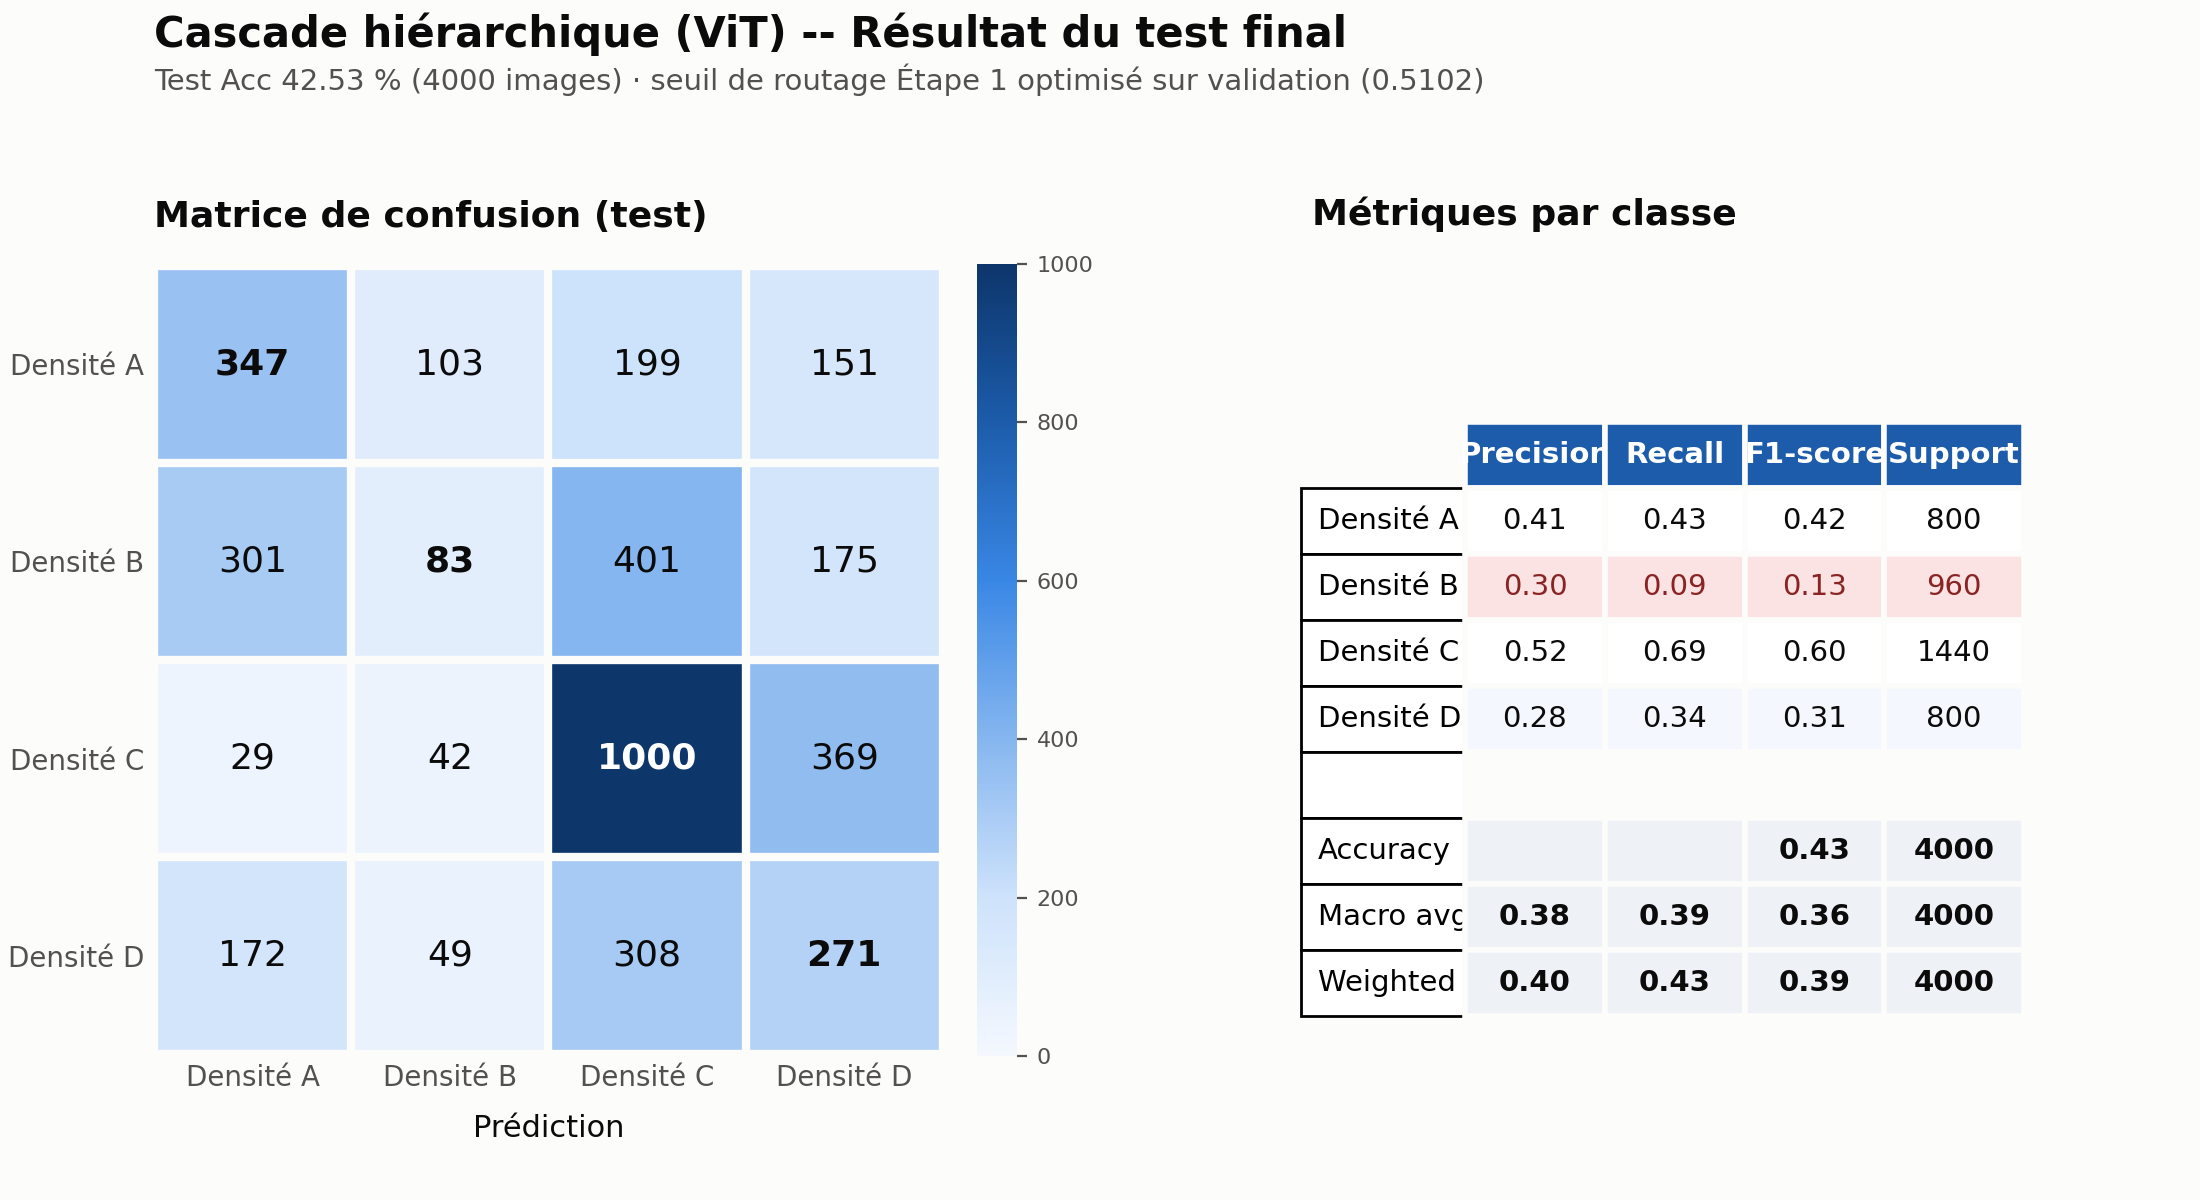
\includegraphics[width=\textwidth]{a7_vit_test}
        \column{0.33\textwidth}
        \centering \small Routage Étape 1\\
        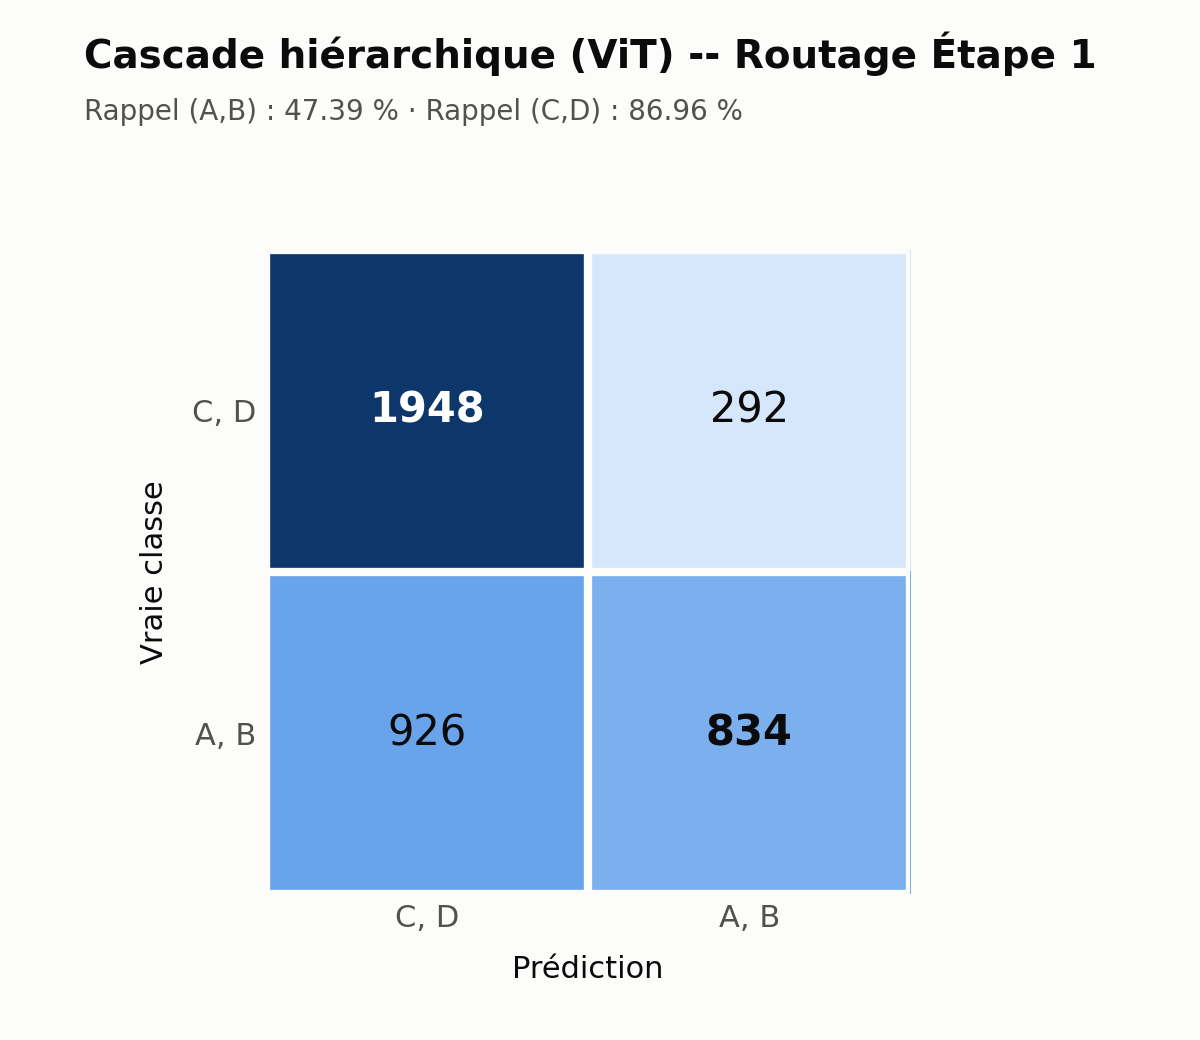
\includegraphics[width=\textwidth]{a7_vit_routage}
        \column{0.33\textwidth}
        \centering \small Modèle 2 isolé\\
        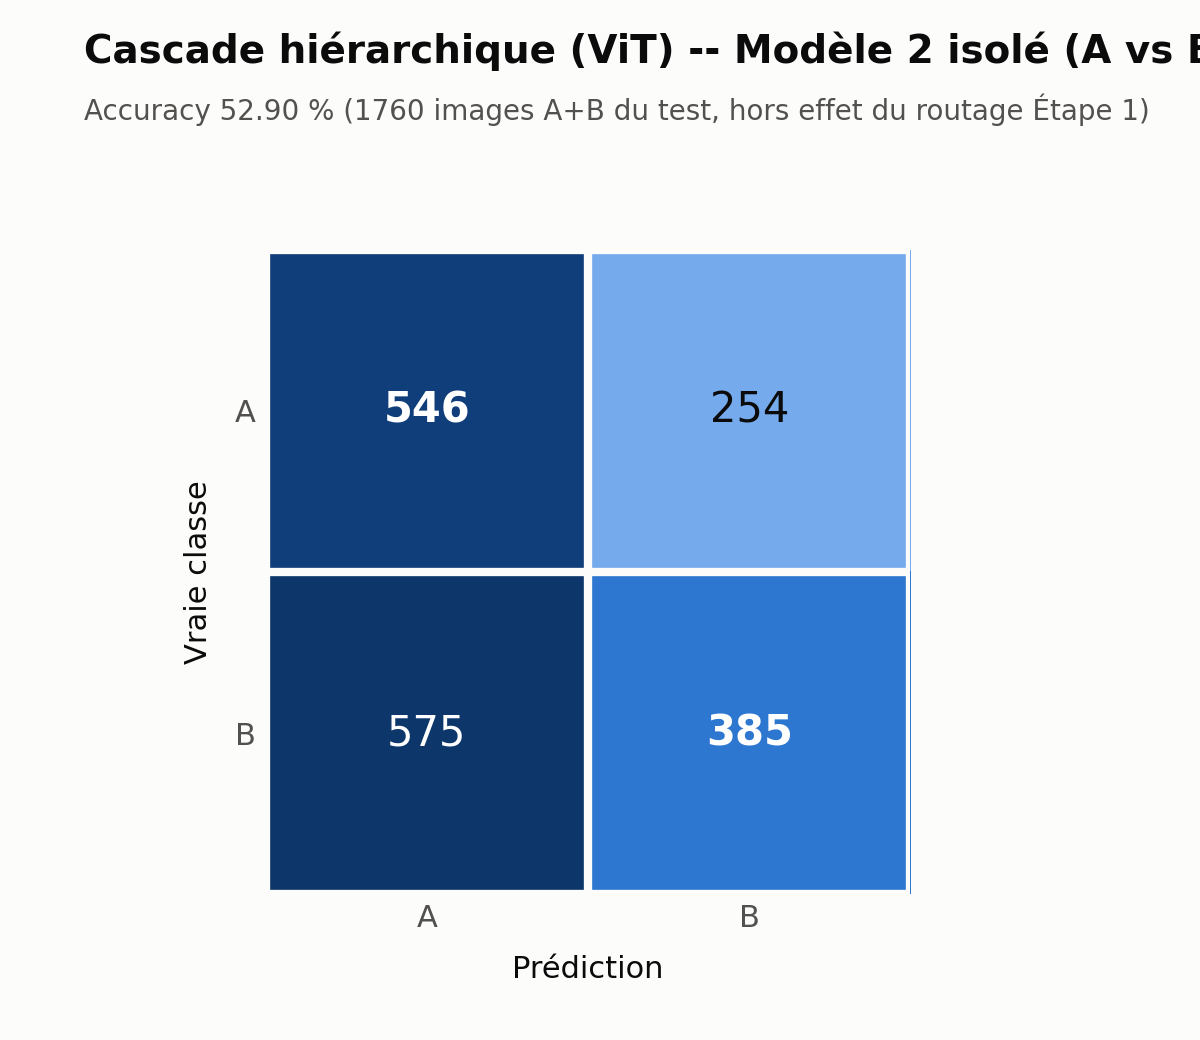
\includegraphics[width=\textwidth]{a7_vit_modele2}
    \end{columns}
\end{frame}

\begin{frame}{Approche 7 -- Cascade hiérarchique (ResNet50)}
    \textbf{Test Acc 48.50\,\%} (4000 images) -- meilleur que ViT, mais toujours en retrait
    \begin{columns}
        \column{0.33\textwidth}
        \centering \small Test final\\
        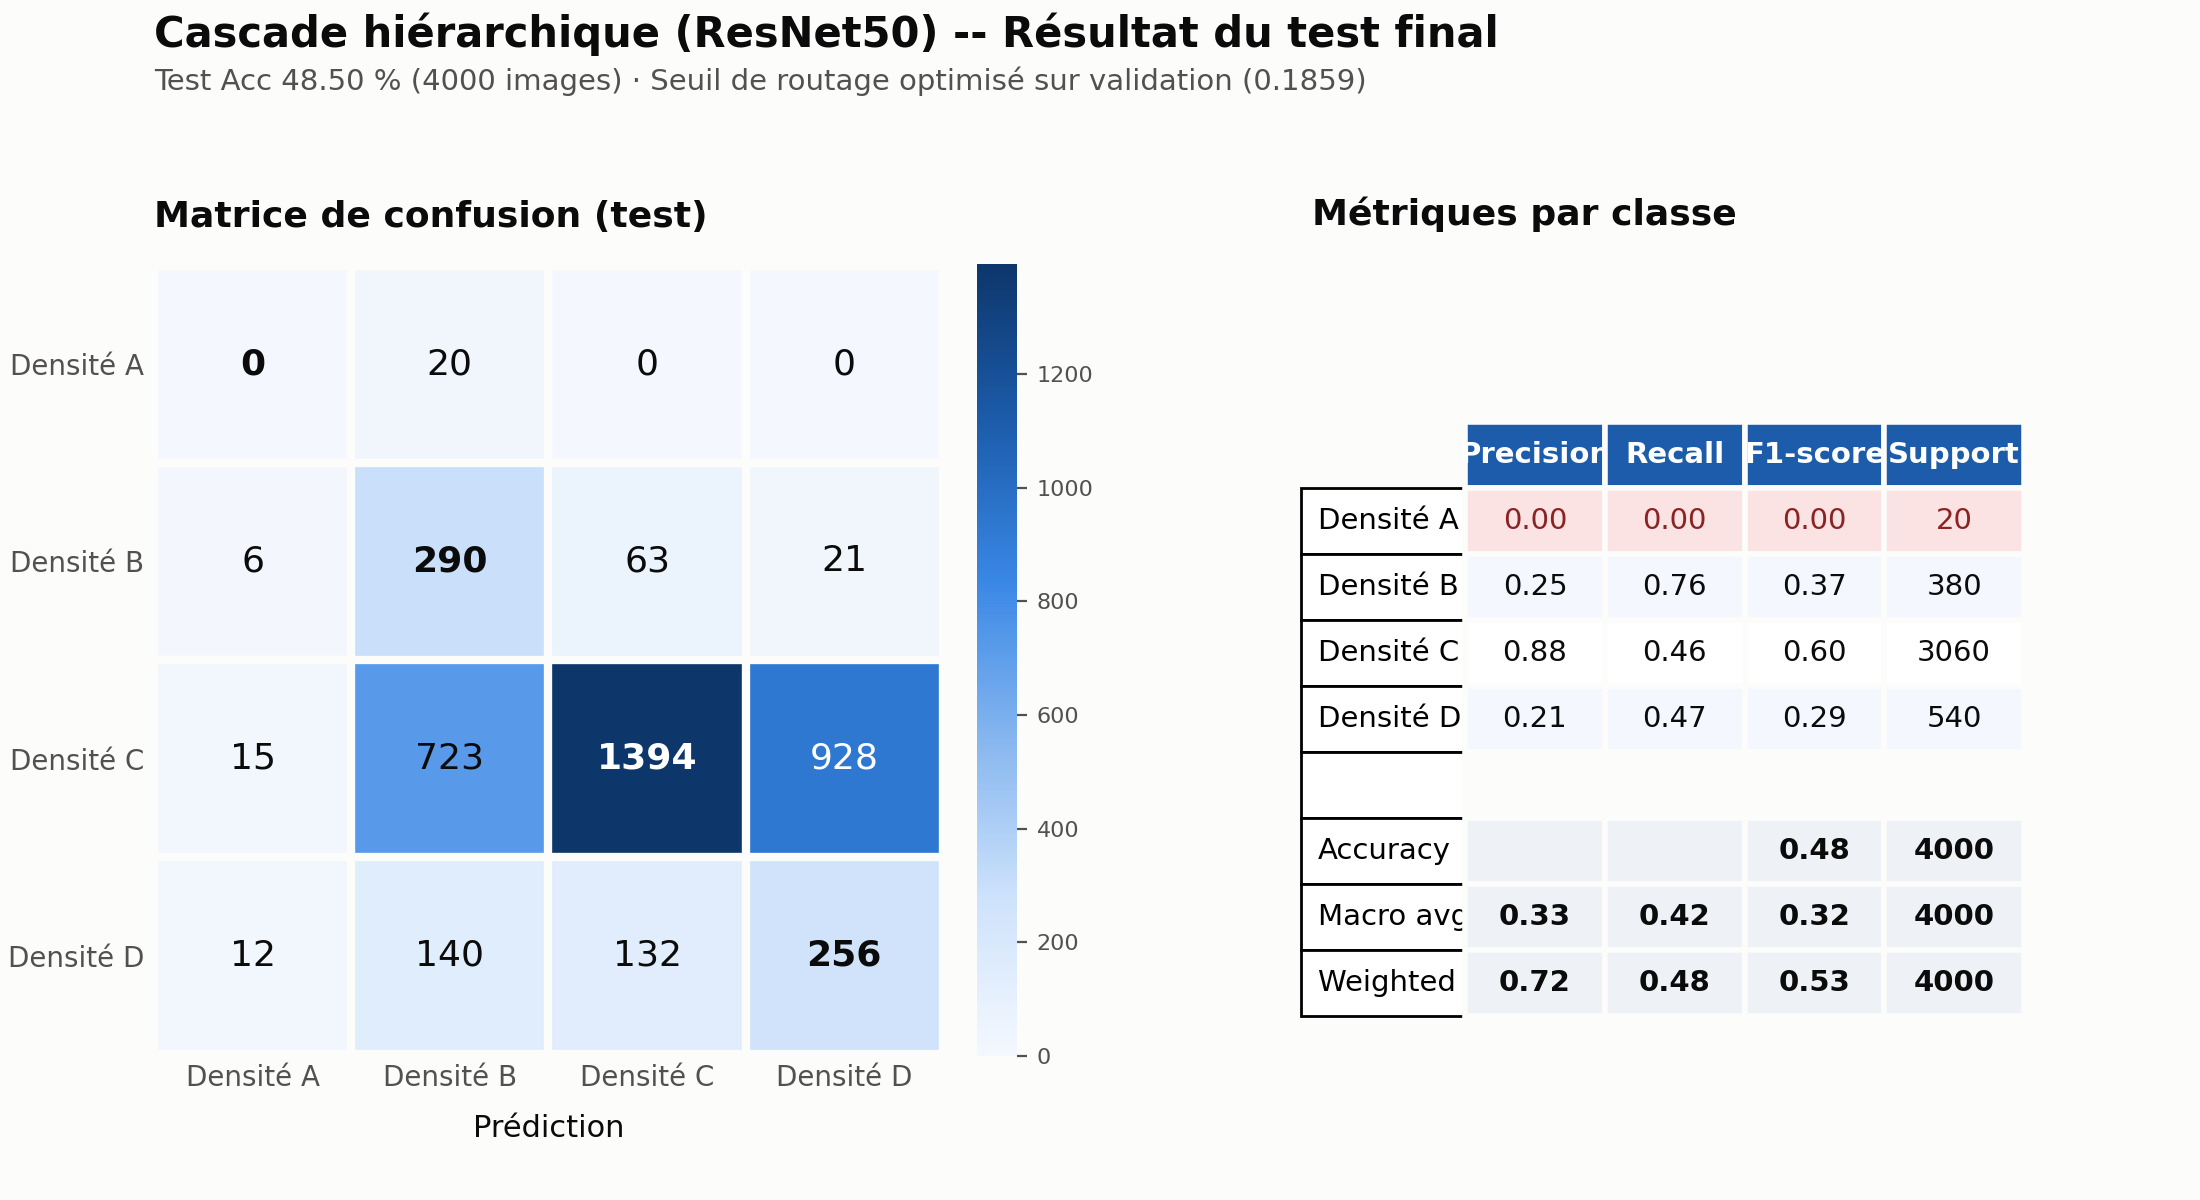
\includegraphics[width=\textwidth]{a7_resnet50_test}
        \column{0.33\textwidth}
        \centering \small Routage Étape 1\\
        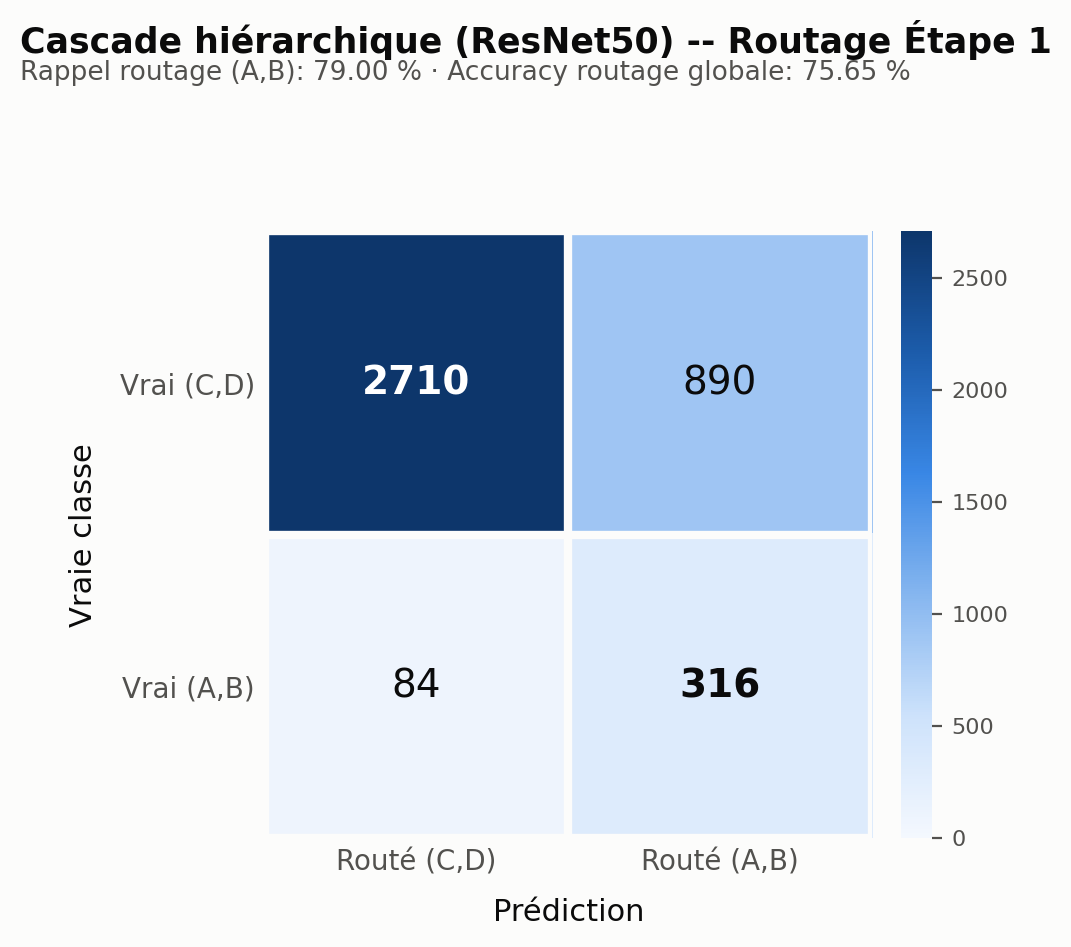
\includegraphics[width=\textwidth]{a7_resnet50_routage}
        \column{0.33\textwidth}
        \centering \small Modèle 2 isolé\\
        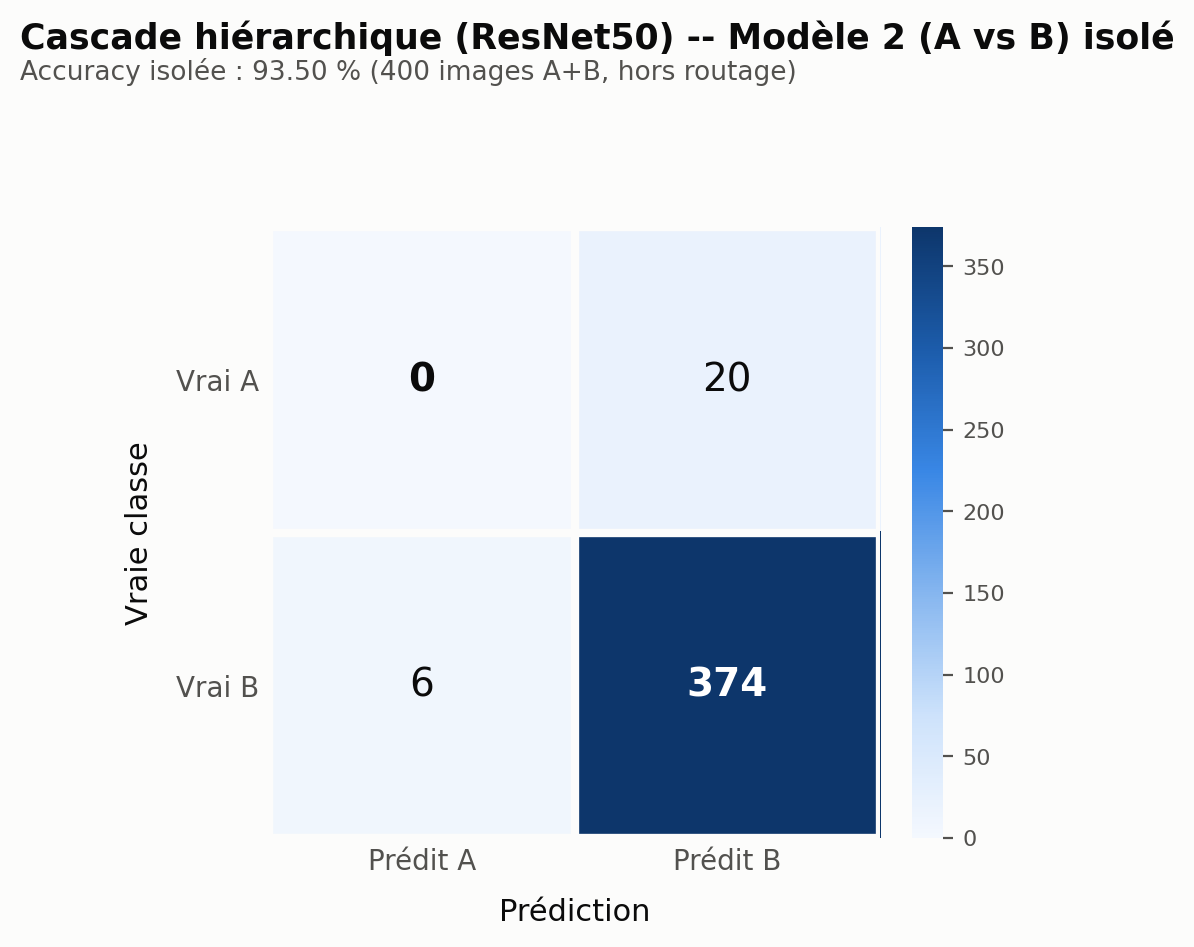
\includegraphics[width=\textwidth]{a7_resnet50_modele2}
    \end{columns}
    \vspace{0.2cm}
    \small Maillon faible différent selon le backbone : Modèle 2 (A vs B) pour ViT, Modèle 3 (C vs D) pour ResNet50.
\end{frame}

% ============================================================================
\section{Approche 8 -- Ensemble (fusion tardive)}
\begin{frame}{Approche 8 -- Ensemble par fusion tardive (Approche 2 + Approche 3)}
    \[
      p_{\text{ens}}(x) = \frac{1}{2}\Big(p^{(2)}(x) + p^{(3)}(x)\Big), \qquad
      \hat{y}_{\text{ens}}(x) = \operatorname*{arg\,max}_{c} \; p_{\text{ens},c}(x)
    \]
    \textbf{Test Acc 80.55\,\%} (2000 images MLO) -- meilleur macro F1 des trois (0.62), rappel classe A : 0 \% $\to$ 30\,\%
    \begin{center}
        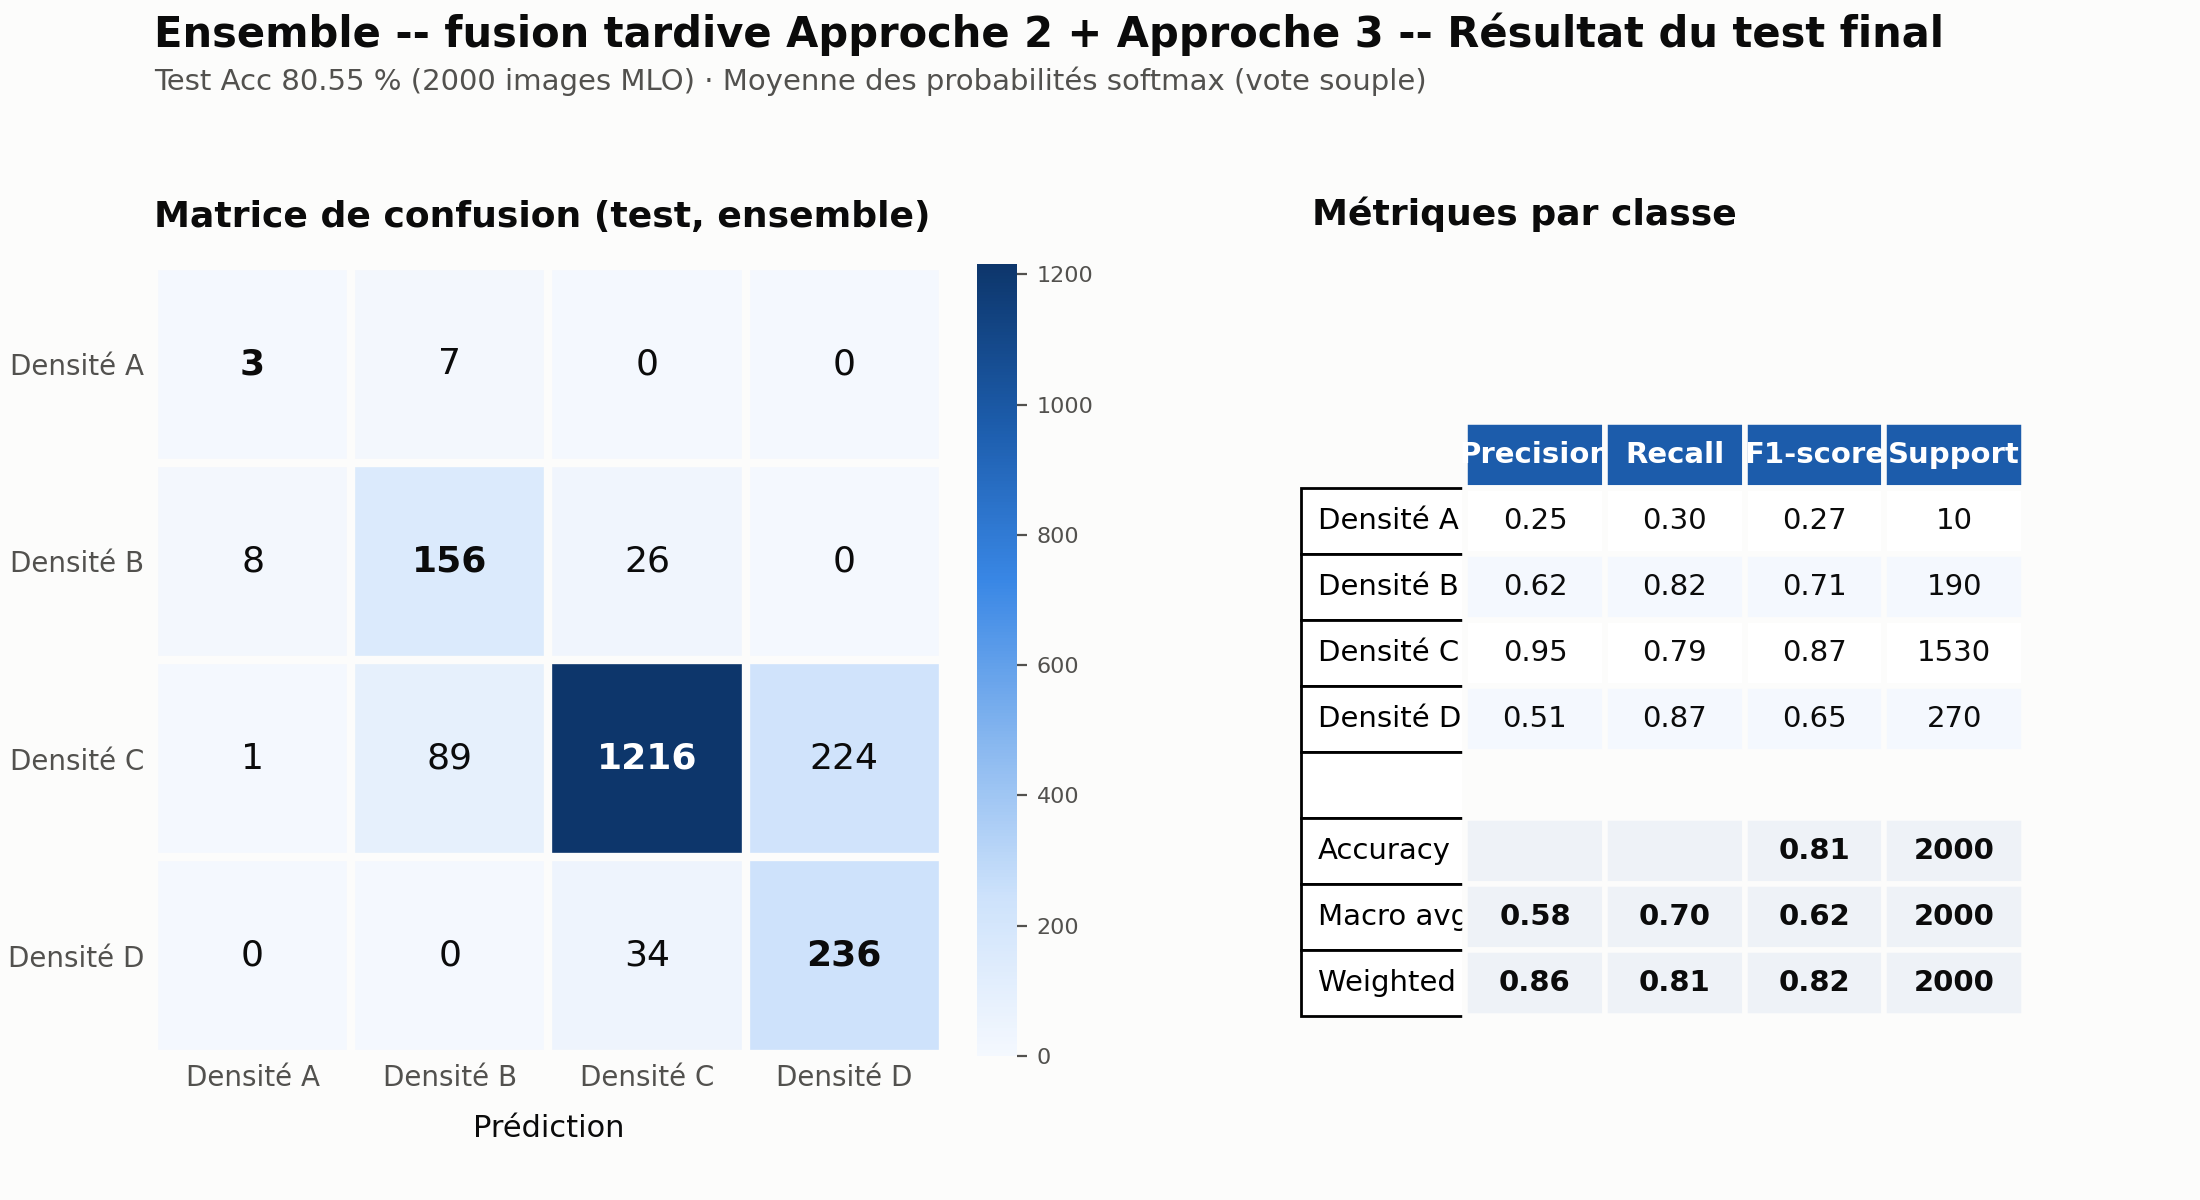
\includegraphics[width=0.65\textwidth]{a8_test}
    \end{center}
\end{frame}

% ============================================================================
\section{Apprentissage fédéré (FedAvg)}
\begin{frame}{FedAvg -- Conception}
    \begin{itemize}
        \item Client H1 : VinDr-Mammo (6801 images d'entraînement)
        \item Client H2 : DDSM/CBIS-DDSM (531 images d'entraînement) -- substitut du réseau HELORA (données non accessibles)
        \item Modèle unique : ResNet50, une seule branche (contrainte du protocole FedAvg)
    \end{itemize}
    \begin{figure}[H]
    \centering
    \begin{tikzpicture}[
        scale=0.6, every node/.style={scale=0.6},
        node distance=1.3cm and 0.5cm,
        server/.style={rectangle, draw, fill=blue!10, text width=5.8cm, align=center, rounded corners, minimum height=1.1cm, font=\small\bfseries},
        client/.style={rectangle, draw, fill=green!10, text width=4.2cm, align=center, rounded corners, minimum height=1.1cm, font=\small},
        arrow/.style={-Stealth, thick, line width=1.2pt},
        labelstyle/.style={font=\scriptsize, color=black!80, align=center}
    ]
        \node (server) [server] {Serveur central \\ (simulation locale sur le cluster) \\ \textnormal{Agrégation : $W_{t+1} = \sum \frac{n_k}{n} W_t^k$}};
        \node (client1) [client, below left=of server] {Client H1 \\ VinDr-Mammo (public) \\ \textnormal{6801 images d'entraînement}};
        \node (client2) [client, below right=of server] {Client H2 \\ DDSM/CBIS-DDSM (public) \\ \textnormal{531 images d'entraînement}};
        \draw [arrow, color=blue!70!black] (server.west) -| node[labelstyle, left, pos=0.3] {1. Envoi du modèle \\ global ($W_t$)} (client1.north);
        \draw [arrow, color=blue!70!black] (server.east) -| node[labelstyle, right, pos=0.3] {1. Envoi du modèle \\ global ($W_t$)} (client2.north);
        \draw [arrow, color=orange!80!black] (client1.south) |- ++(0,-0.8) -| node[labelstyle, left, pos=0.7] {2. Renvoi des poids \\ entraînés ($W_t^1$)} (server.south);
        \draw [arrow, color=orange!80!black] (client2.south) |- ++(0,-0.8) -| node[labelstyle, right, pos=0.7] {2. Renvoi des poids \\ entraînés ($W_t^2$)} (server.south);
    \end{tikzpicture}
    \end{figure}
\end{frame}

\begin{frame}{FedAvg -- Algorithme}
    \begin{algorithm}[H]
    \scriptsize
    \caption{FedAvg -- apprentissage fédéré entre les clients H1 et H2}
    \begin{algorithmic}[1]
    \Procedure{ServeurFedAvg}{}
      \State Initialiser les poids globaux $W_0$ (ResNet50, ImageNet)
      \For{chaque round $t = 1, \dots, T$}
        \For{chaque client $k \in \{\text{H1}, \text{H2}\}$}
          \State $W_t^k \gets$ \Call{ClientUpdate}{$k$, $W_{t-1}$}
        \EndFor
        \State $W_t \gets \sum_{k} \dfrac{n_k}{n}\, W_t^k$
        \Comment{agrégation pondérée par la taille locale $n_k$}
      \EndFor
      \State \Return $W_T$
    \EndProcedure
    \Procedure{ClientUpdate}{$k$, $W$}
      \For{chaque époque locale $e = 1, \dots, E$}
        \For{chaque mini-lot $b$ du client $k$}
          \State $W \gets W - \eta \nabla_W \mathcal{L}(W; b)$
        \EndFor
      \EndFor
      \State \Return $W$ au serveur
    \EndProcedure
    \end{algorithmic}
    \end{algorithm}
    \small $E{=}1$ époque locale par round (15 rounds au total).
\end{frame}

\begin{frame}{FedAvg -- Résultats (15 rounds)}
    \begin{columns}
        \column{0.5\textwidth}
        \centering \small Accuracy de validation\\
        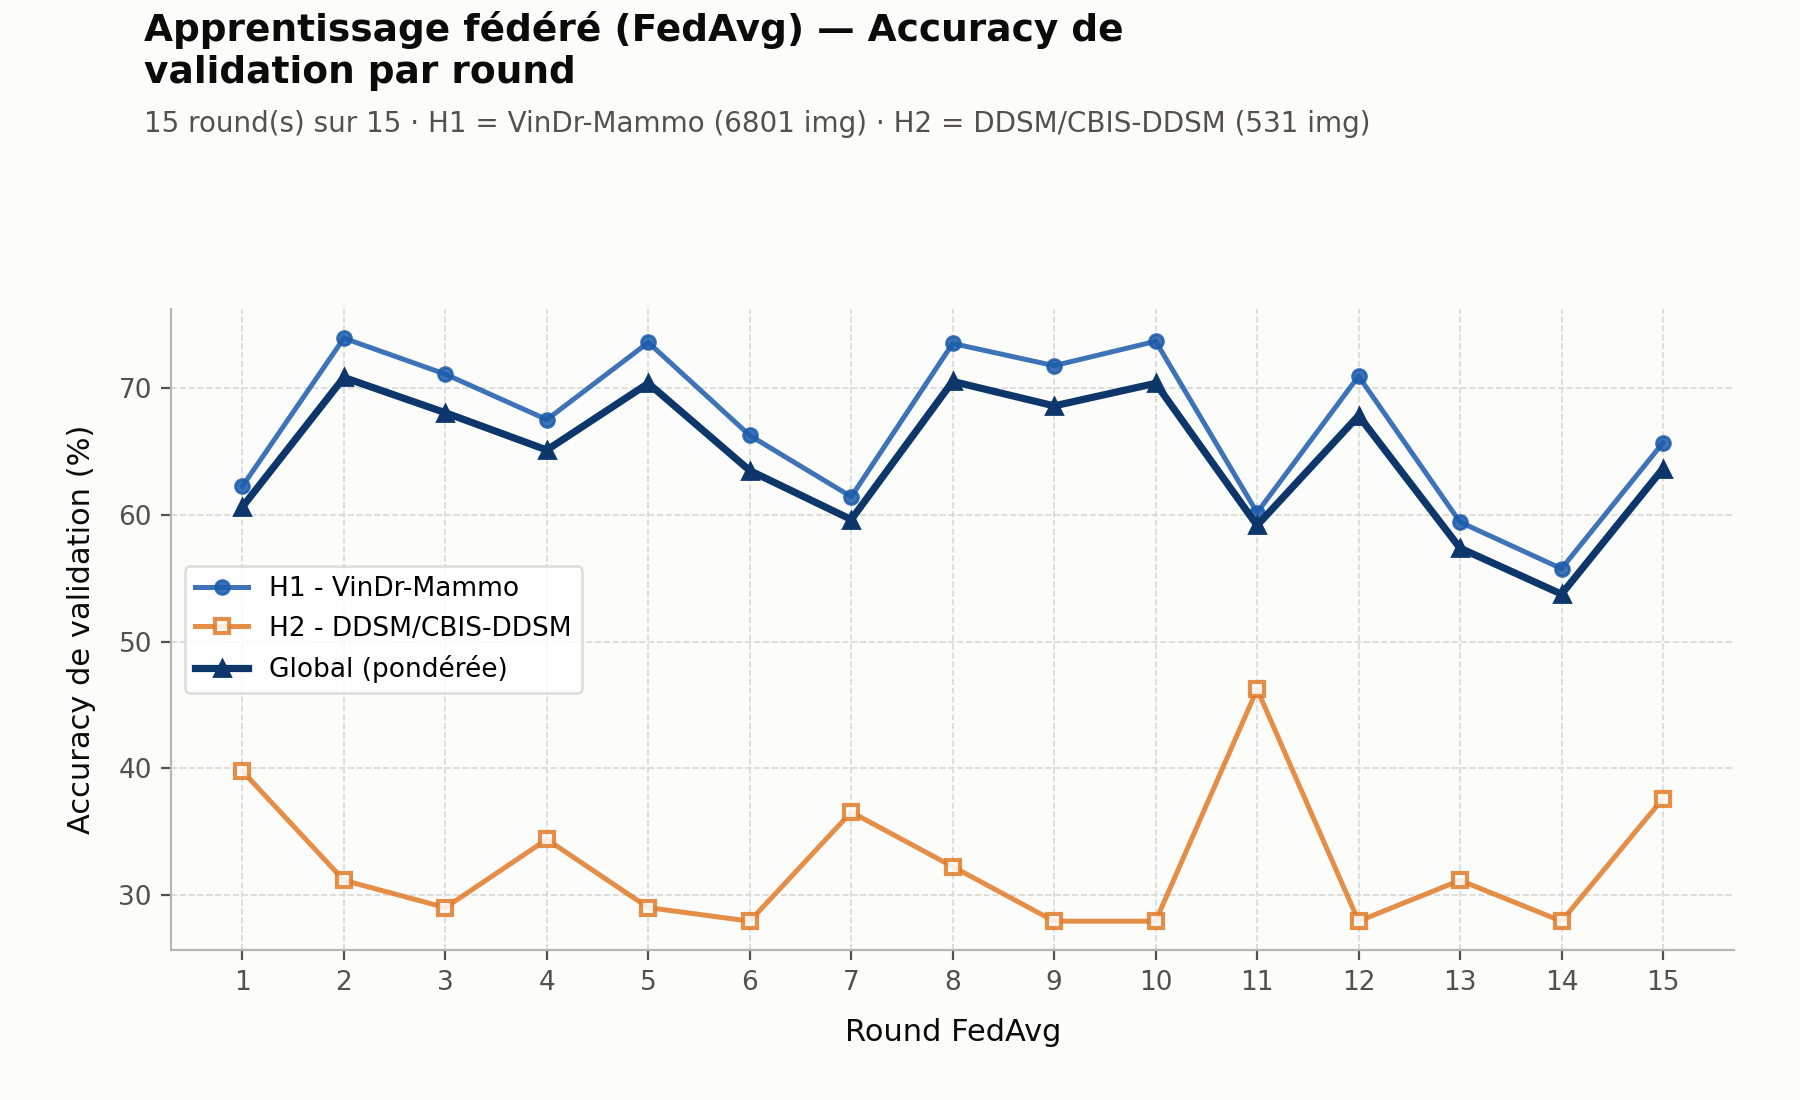
\includegraphics[width=\textwidth]{fed_accuracy}
        \column{0.5\textwidth}
        \centering \small Loss de validation\\
        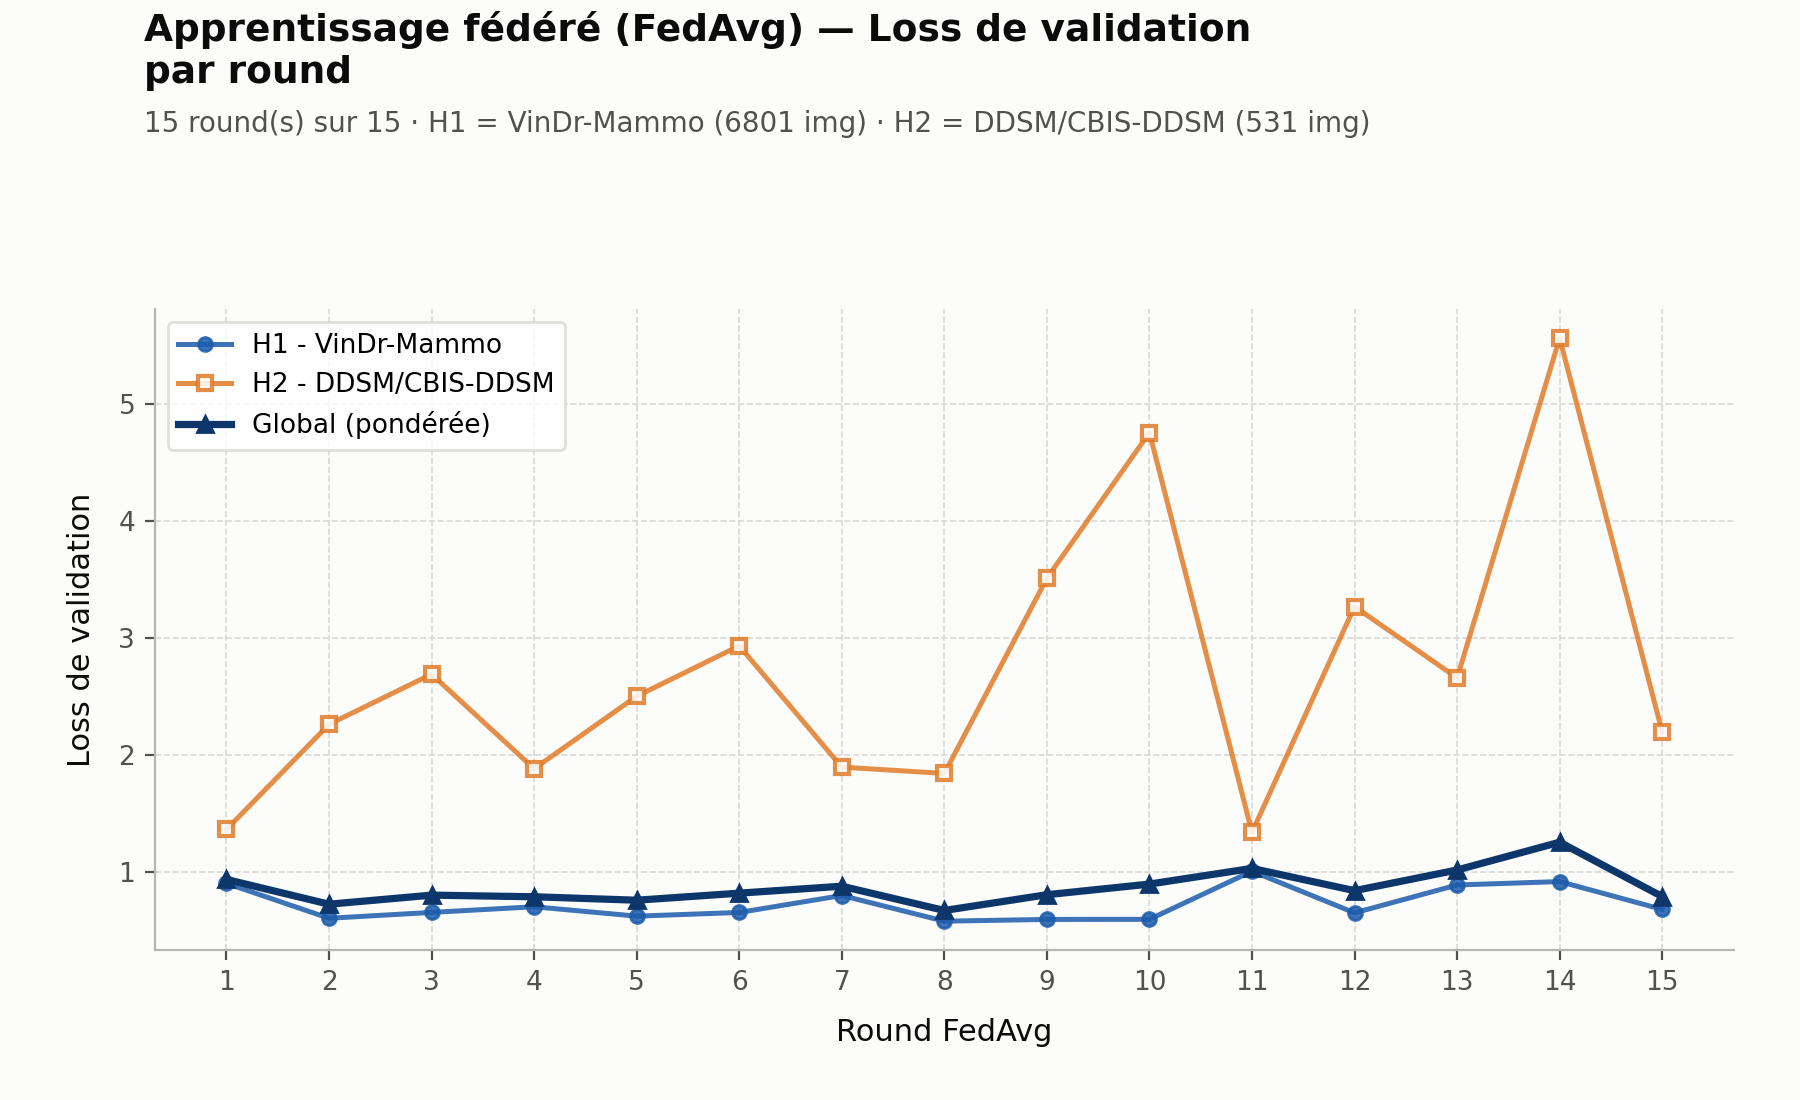
\includegraphics[width=\textwidth]{fed_loss}
    \end{columns}
    \small Accuracy globale entre 53.74\,\% (Round 14) et 70.82\,\% (Round 2) -- pas de convergence stable, $H1$ (93\,\% du poids d'agrégation) domine largement $H2$.
\end{frame}

\begin{frame}{FedAvg -- Comparaison avec une baseline centralisée}
    \begin{table}
    \centering
    \begin{tabular}{lrr}
        \toprule
        Source & Test Acc (centralisé) & FedAvg (val, 15 rounds) \\
        \midrule
        VinDr-Mammo & \textbf{82.30\,\%} & 53.74\,\% -- 70.82\,\% \\
        DDSM/CBIS-DDSM & 31.17\,\% & 27.96\,\% -- 46.24\,\% \\
        \bottomrule
    \end{tabular}
    \end{table}
    \begin{itemize}
        \item Sur VinDr : la fédération coûte réellement de la performance (5 époques centralisées vs 1 seule par round en fédéré)
        \item Sur DDSM : même fourchette que FedAvg -- la faiblesse vient d'un décalage de domaine (films scannés vs numérique natif), pas de la fédération elle-même
    \end{itemize}
\end{frame}

% ============================================================================
\section{Interprétabilité -- Approche 3}
\begin{frame}{Interprétabilité -- t-SNE (Approche 3)}
    Espace latent (avant-dernière couche) projeté en 2D
    \begin{center}
        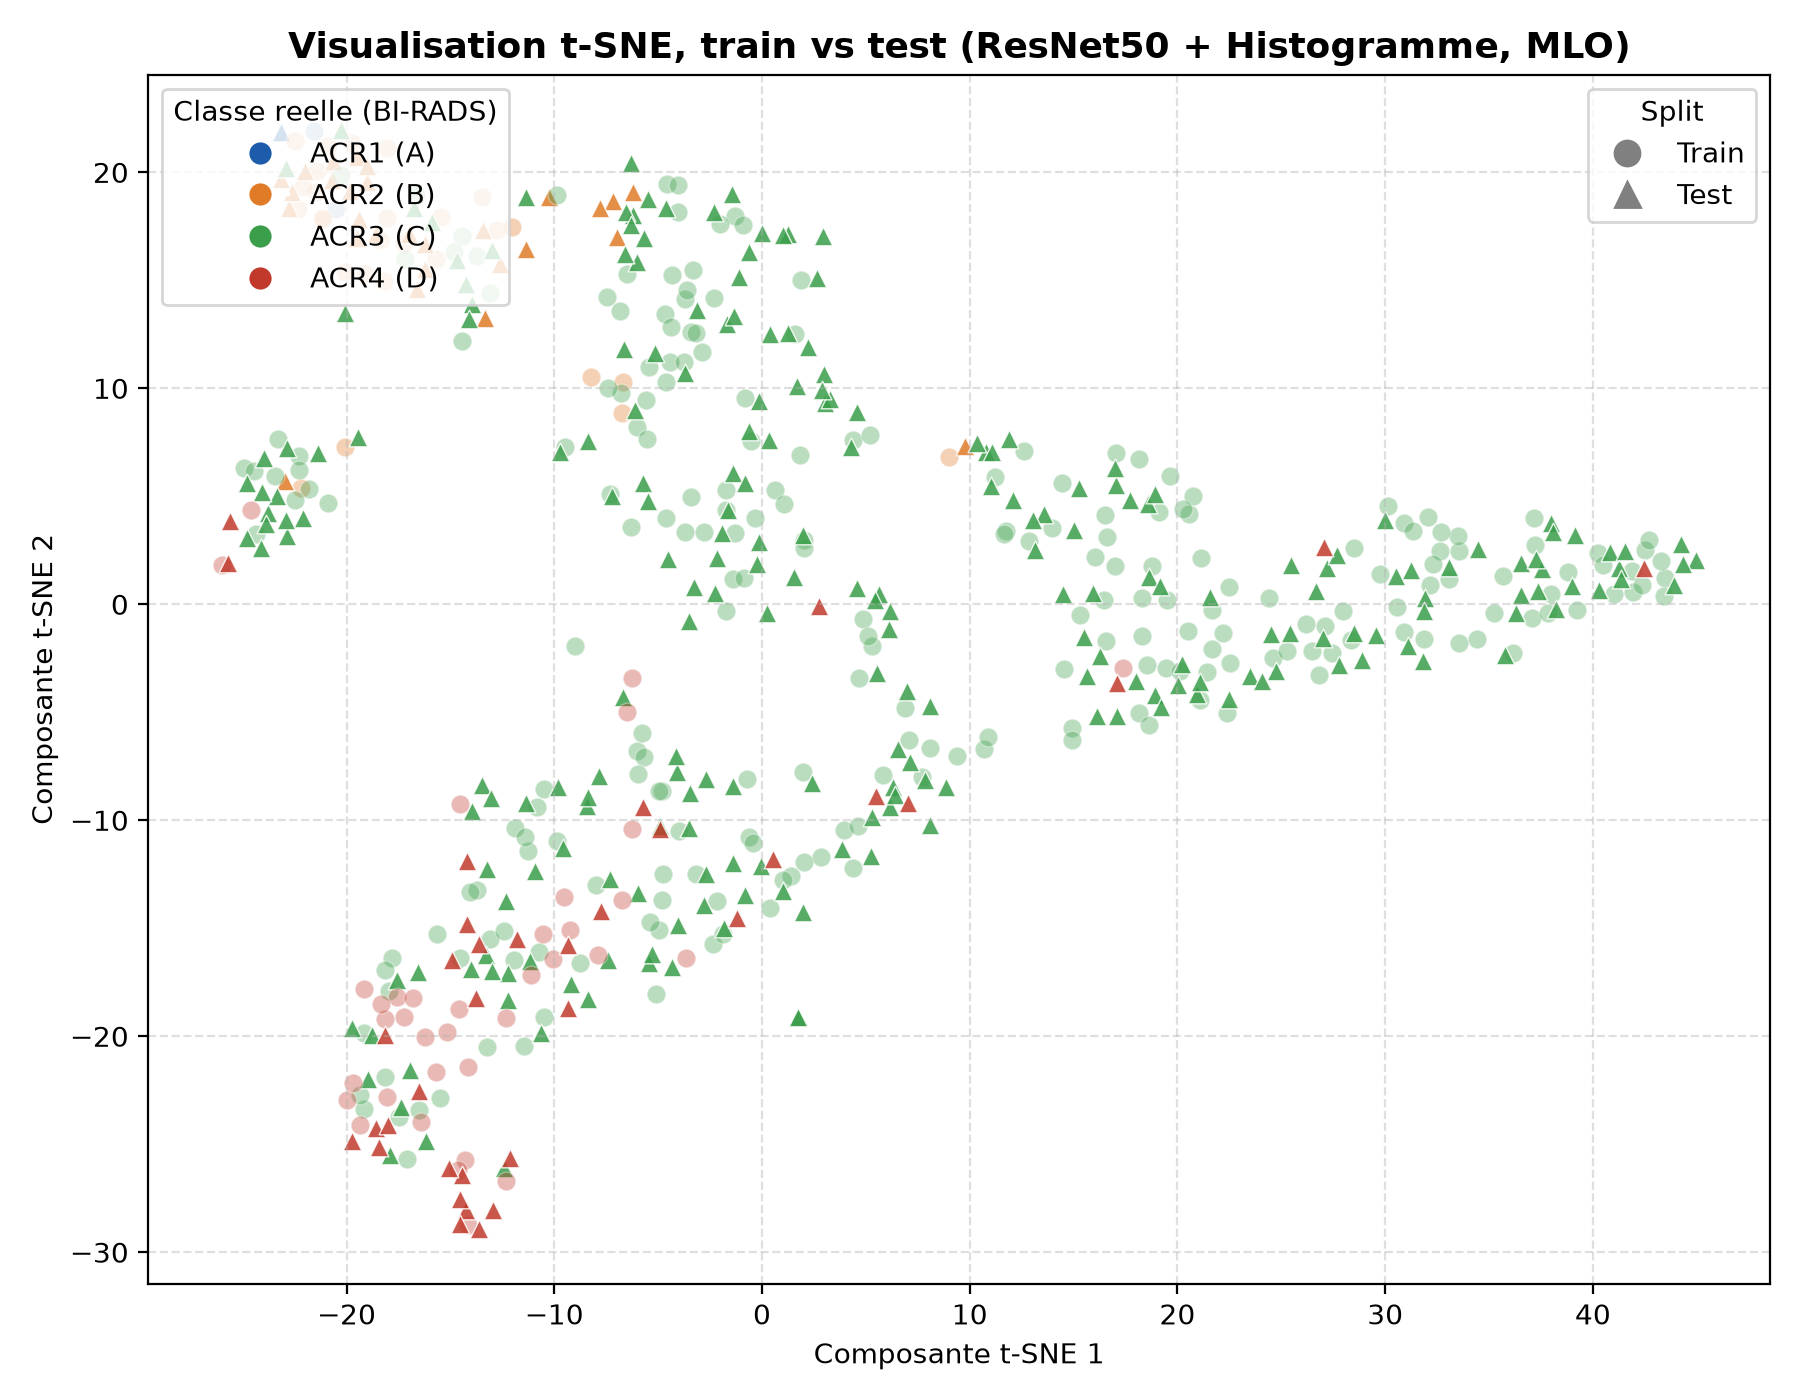
\includegraphics[width=0.5\textwidth]{a3_tsne}
    \end{center}
    \small B et D forment des zones assez distinctes ; C domine l'espace ; A trop rare pour conclure.
\end{frame}

\begin{frame}{Interprétabilité -- Grad-CAM (Approche 3)}
    \footnotesize 3 exemples par classe -- vérification de la stabilité du comportement du modèle
    \begin{center}
        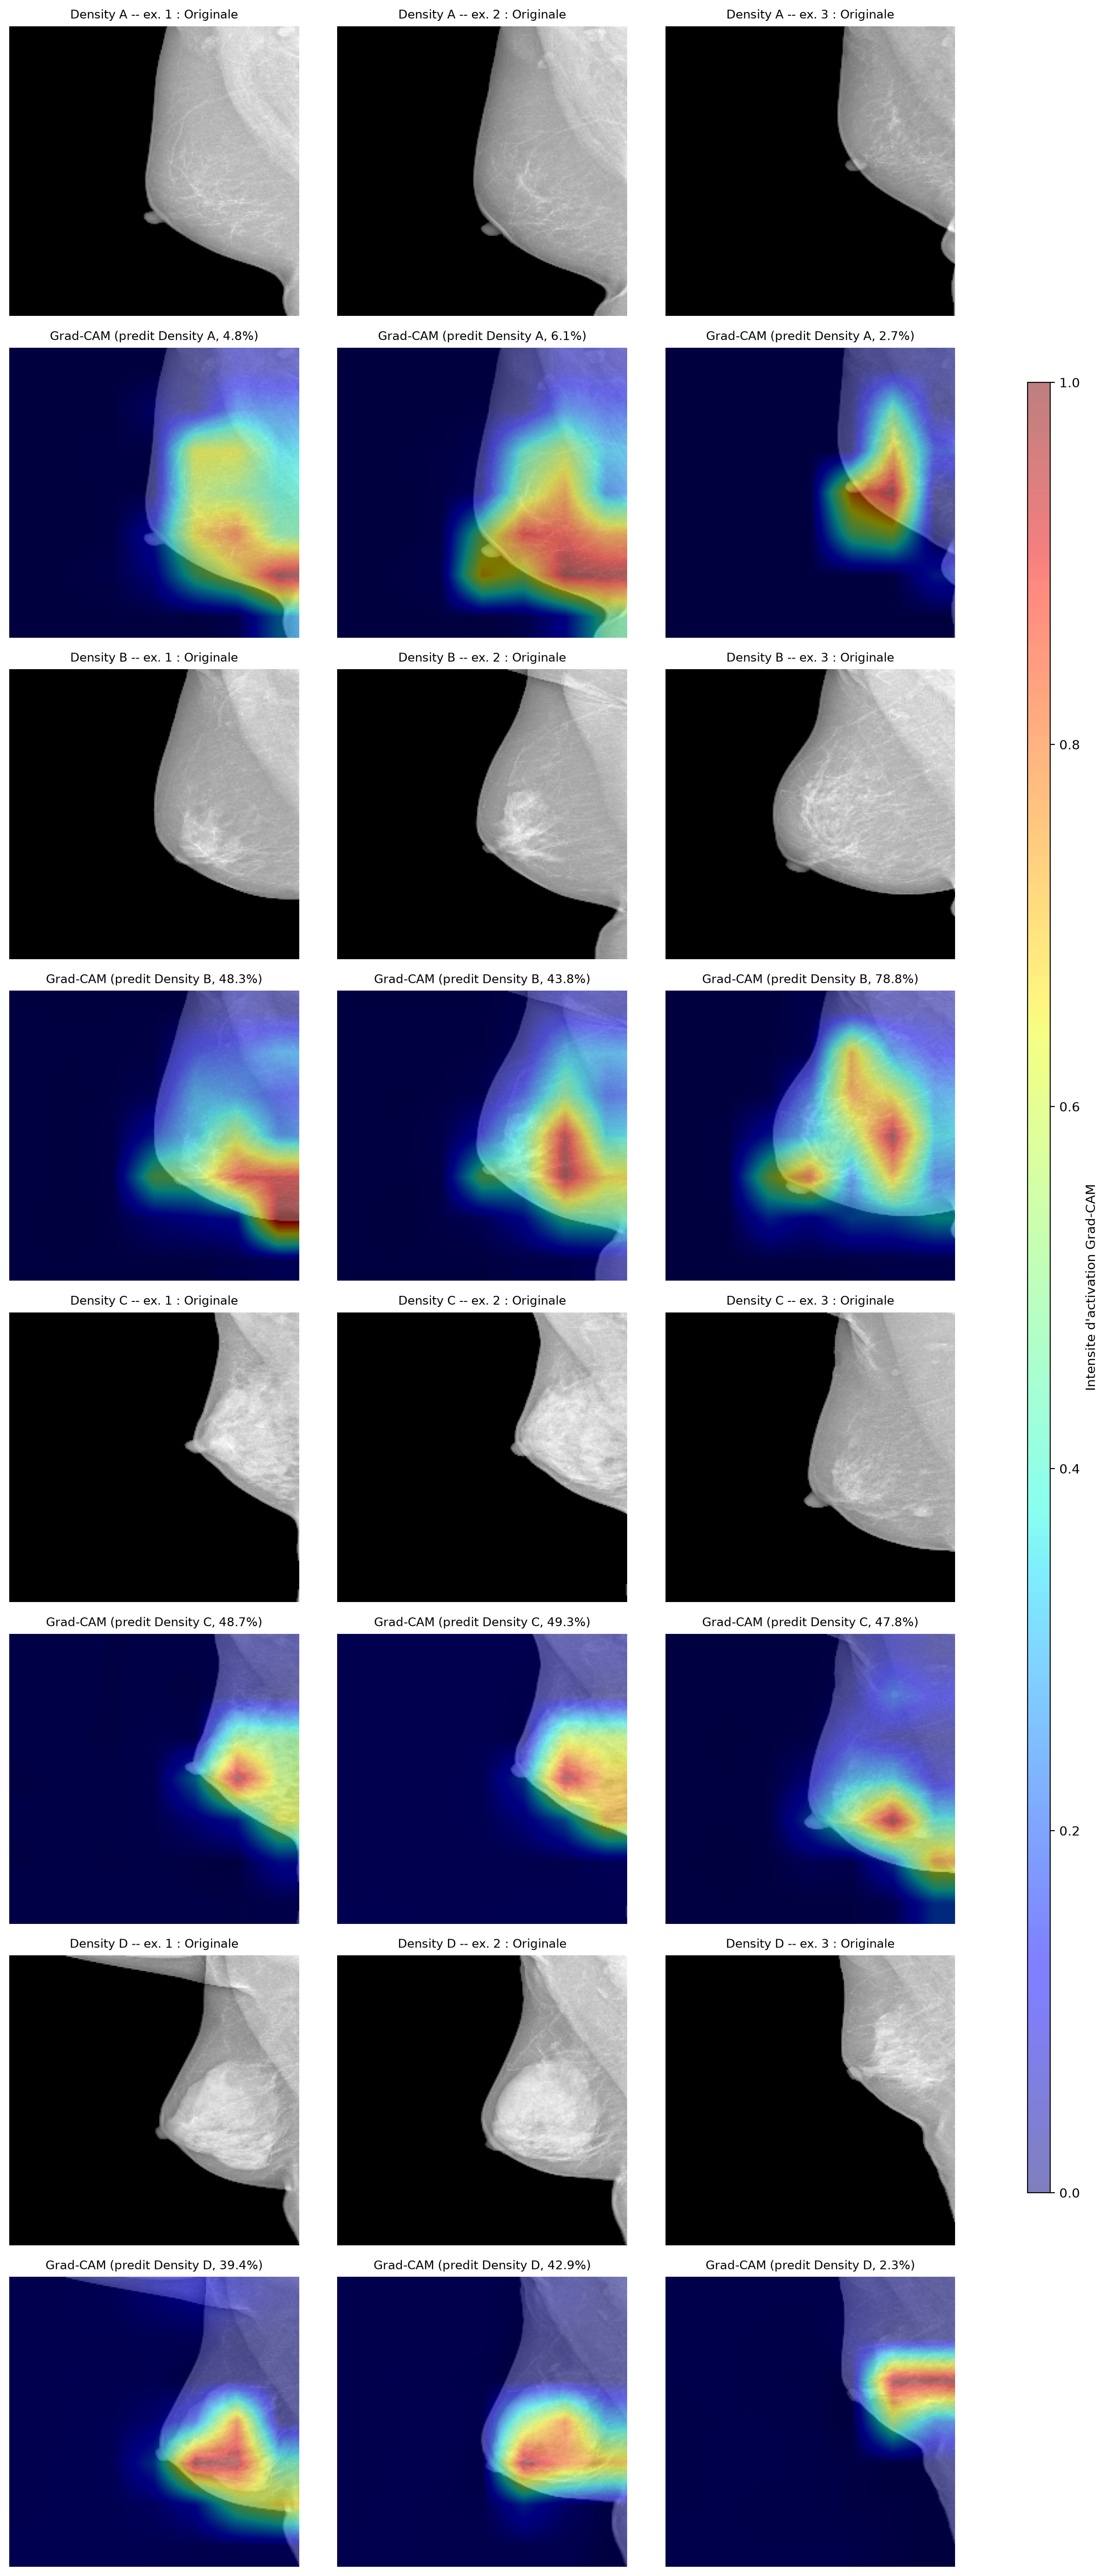
\includegraphics[height=0.74\textheight]{a3_gradcam}
    \end{center}
    \footnotesize Classe C : foyer stable près du mamelon ($\sim$48\,\%). Classe D : 2/3 exemples corrects, 1/3 s'effondre (2.3\,\%). Classe A : constamment faible (2.7--6.1\,\%).
\end{frame}

\begin{frame}{Merci}
    \centering
    \Large Merci de votre attention \\[0.5cm]
    \normalsize Questions / discussion
\end{frame}

\end{document}
